%%%%%%%%%%%%%%%%%%%%%%%%%%%%%%%%%%%%%%%%%
% The Legrand Orange Book
% LaTeX Template
% Version 2.4 (26/09/2018)
%
% This template was downloaded from:
% http://www.LaTeXTemplates.com
%
% Original author:
% Mathias Legrand (legrand.mathias@gmail.com) with modifications by:
% Vel (vel@latextemplates.com)
%
% License:
% CC BY-NC-SA 3.0 (http://creativecommons.org/licenses/by-nc-sa/3.0/)
%
% Compiling this template:
% This template uses biber for its bibliography and makeindex for its index.
% When you first open the template, compile it from the command line with the 
% commands below to make sure your LaTeX distribution is configured correctly:
%
% 1) pdflatex main
% 2) makeindex main.idx -s StyleInd.ist
% 3) biber main
% 4) pdflatex main x 2
%
% After this, when you wish to update the bibliography/index use the appropriate
% command above and make sure to compile with pdflatex several times 
% afterwards to propagate your changes to the document.
%
% This template also uses a number of packages which may need to be
% updated to the newest versions for the template to compile. It is strongly
% recommended you update your LaTeX distribution if you have any
% compilation errors.
%
% Important note:
% Chapter heading images should have a 2:1 width:height ratio,
% e.g. 920px width and 460px height.
%
%%%%%%%%%%%%%%%%%%%%%%%%%%%%%%%%%%%%%%%%%

%----------------------------------------------------------------------------------------
%	PACKAGES AND OTHER DOCUMENT CONFIGURATIONS
%----------------------------------------------------------------------------------------

\documentclass[11pt,fleqn]{book} % Default font size and left-justified equations

%%%%%%%%%%%%%%%%%%%%%%%%%%%%%%%%%%%%%%%%%
% The Legrand Orange Book
% Structural Definitions File
% Version 2.1 (26/09/2018)
%
% Original author:
% Mathias Legrand (legrand.mathias@gmail.com) with modifications by:
% Vel (vel@latextemplates.com)
% 
% This file was downloaded from:
% http://www.LaTeXTemplates.com
%
% License:
% CC BY-NC-SA 3.0 (http://creativecommons.org/licenses/by-nc-sa/3.0/)
%
%%%%%%%%%%%%%%%%%%%%%%%%%%%%%%%%%%%%%%%%%

%----------------------------------------------------------------------------------------
%	VARIOUS REQUIRED PACKAGES AND CONFIGURATIONS
%----------------------------------------------------------------------------------------

\usepackage{graphicx} % Required for including pictures
\graphicspath{{Pictures/}} % Specifies the directory where pictures are stored

\usepackage{lipsum} % Inserts dummy text

\usepackage{tikz} % Required for drawing custom shapes

\usepackage[english]{babel} % English language/hyphenation

\usepackage{enumitem} % Customize lists
\setlist{nolistsep} % Reduce spacing between bullet points and numbered lists

\usepackage{booktabs} % Required for nicer horizontal rules in tables

\usepackage{xcolor} % Required for specifying colors by name
%\definecolor{ocre}{RGB}{40,122,255} % Define the orange color used for highlighting throughout the book
%\definecolor{ocre}{RGB}{20,30,150}			% A more neutral blue
\definecolor{ocre}{HTML}{2879c7}		%ippbleu

%----------------------------------------------------------------------------------------
%	MARGINS
%----------------------------------------------------------------------------------------

\usepackage{geometry} % Required for adjusting page dimensions and margins

\geometry{
	paper=a4paper, % Paper size, change to letterpaper for US letter size
	top=3cm, % Top margin
	bottom=3cm, % Bottom margin
	left=3cm, % Left margin
	right=3cm, % Right margin
	headheight=14pt, % Header height
	footskip=1.4cm, % Space from the bottom margin to the baseline of the footer
	headsep=10pt, % Space from the top margin to the baseline of the header
	%showframe, % Uncomment to show how the type block is set on the page
}

%----------------------------------------------------------------------------------------
%	FONTS
%----------------------------------------------------------------------------------------

% \usepackage{avant} % Use the Avantgarde font for headings
\usepackage{times} % Use the Times font for headings
\usepackage{mathptmx} % Use the Adobe Times Roman as the default text font together with math symbols from the Sym­bol, Chancery and Com­puter Modern fonts

\usepackage{microtype} % Slightly tweak font spacing for aesthetics
\usepackage[utf8]{inputenc} % Required for including letters with accents
\usepackage[T1]{fontenc} % Use 8-bit encoding that has 256 glyphs

%----------------------------------------------------------------------------------------
%	BIBLIOGRAPHY AND INDEX
%----------------------------------------------------------------------------------------

\usepackage[style=numeric,citestyle=numeric,sorting=nyt,sortcites=true,autopunct=true,babel=hyphen,hyperref=true,abbreviate=false,backref=true,backend=biber]{biblatex}
\addbibresource{bibliography.bib} % BibTeX bibliography file
\defbibheading{bibempty}{}

\usepackage{calc} % For simpler calculation - used for spacing the index letter headings correctly
\usepackage{makeidx} % Required to make an index
\makeindex % Tells LaTeX to create the files required for indexing

%----------------------------------------------------------------------------------------
%	MAIN TABLE OF CONTENTS
%----------------------------------------------------------------------------------------

\usepackage{titletoc} % Required for manipulating the table of contents

\contentsmargin{0cm} % Removes the default margin

% Part text styling (this is mostly taken care of in the PART HEADINGS section of this file)
\titlecontents{part}
	[0cm] % Left indentation
	{\addvspace{20pt}\bfseries} % Spacing and font options for parts
	{}
	{}
	{}

% Chapter text styling
\titlecontents{chapter}
	[1.25cm] % Left indentation
	{\addvspace{12pt}\large\sffamily\bfseries} % Spacing and font options for chapters
	{\color{ocre!60}\contentslabel[\Large\thecontentslabel]{1.25cm}\color{ocre}} % Formatting of numbered sections of this type
	{\color{ocre}} % Formatting of numberless sections of this type
	{\color{ocre!60}\normalsize\;\titlerule*[.5pc]{.}\;\thecontentspage} % Formatting of the filler to the right of the heading and the page number

% Section text styling
\titlecontents{section}
	[1.25cm] % Left indentation
	{\addvspace{3pt}\sffamily\bfseries} % Spacing and font options for sections
	{\contentslabel[\thecontentslabel]{1.25cm}} % Formatting of numbered sections of this type
	{} % Formatting of numberless sections of this type
	{\hfill\color{black}\thecontentspage} % Formatting of the filler to the right of the heading and the page number

% Subsection text styling
\titlecontents{subsection}
	[1.25cm] % Left indentation
	{\addvspace{1pt}\sffamily\small} % Spacing and font options for subsections
	{\contentslabel[\thecontentslabel]{1.25cm}} % Formatting of numbered sections of this type
	{} % Formatting of numberless sections of this type
	{\ \titlerule*[.5pc]{.}\;\thecontentspage} % Formatting of the filler to the right of the heading and the page number

% Figure text styling
\titlecontents{figure}
	[1.25cm] % Left indentation
	{\addvspace{1pt}\sffamily\small} % Spacing and font options for figures
	{\thecontentslabel\hspace*{1em}} % Formatting of numbered sections of this type
	{} % Formatting of numberless sections of this type
	{\ \titlerule*[.5pc]{.}\;\thecontentspage} % Formatting of the filler to the right of the heading and the page number

% Table text styling
\titlecontents{table}
	[1.25cm] % Left indentation
	{\addvspace{1pt}\sffamily\small} % Spacing and font options for tables
	{\thecontentslabel\hspace*{1em}} % Formatting of numbered sections of this type
	{} % Formatting of numberless sections of this type
	{\ \titlerule*[.5pc]{.}\;\thecontentspage} % Formatting of the filler to the right of the heading and the page number

%----------------------------------------------------------------------------------------
%	MINI TABLE OF CONTENTS IN PART HEADS
%----------------------------------------------------------------------------------------

% Chapter text styling
\titlecontents{lchapter}
	[0em] % Left indentation
	{\addvspace{15pt}\large\sffamily\bfseries} % Spacing and font options for chapters
	{\color{ocre}\contentslabel[\Large\thecontentslabel]{1.25cm}\color{ocre}} % Chapter number
	{}  
	{\color{ocre}\normalsize\sffamily\bfseries\;\titlerule*[.5pc]{.}\;\thecontentspage} % Page number

% Section text styling
\titlecontents{lsection}
	[0em] % Left indentation
	{\sffamily\small} % Spacing and font options for sections
	{\contentslabel[\thecontentslabel]{1.25cm}} % Section number
	{}
	{}

% Subsection text styling (note these aren't shown by default, display them by searchings this file for tocdepth and reading the commented text)
\titlecontents{lsubsection}
	[.5em] % Left indentation
	{\sffamily\footnotesize} % Spacing and font options for subsections
	{\contentslabel[\thecontentslabel]{1.25cm}}
	{}
	{}

%----------------------------------------------------------------------------------------
%	HEADERS AND FOOTERS
%----------------------------------------------------------------------------------------

\usepackage{fancyhdr} % Required for header and footer configuration

\pagestyle{fancy} % Enable the custom headers and footers

\renewcommand{\chaptermark}[1]{\markboth{\sffamily\normalsize\bfseries\chaptername\ \thechapter.\ #1}{}} % Styling for the current chapter in the header
\renewcommand{\sectionmark}[1]{\markright{\sffamily\normalsize\thesection\hspace{5pt}#1}{}} % Styling for the current section in the header

\fancyhf{} % Clear default headers and footers
\fancyhead[LE,RO]{\sffamily\normalsize\thepage} % Styling for the page number in the header
\fancyhead[LO]{\rightmark} % Print the nearest section name on the left side of odd pages
\fancyhead[RE]{\leftmark} % Print the current chapter name on the right side of even pages
%\fancyfoot[C]{\thepage} % Uncomment to include a footer

\renewcommand{\headrulewidth}{0.5pt} % Thickness of the rule under the header

\fancypagestyle{plain}{% Style for when a plain pagestyle is specified
	\fancyhead{}\renewcommand{\headrulewidth}{0pt}%
}

% Removes the header from odd empty pages at the end of chapters
\makeatletter
\renewcommand{\cleardoublepage}{
\clearpage\ifodd\c@page\else
\hbox{}
\vspace*{\fill}
\thispagestyle{empty}
%\newpage
\fi}

%----------------------------------------------------------------------------------------
%	THEOREM STYLES
%----------------------------------------------------------------------------------------

\usepackage{amsmath,amsfonts,amssymb,amsthm} % For math equations, theorems, symbols, etc

\newcommand{\intoo}[2]{\mathopen{]}#1\,;#2\mathclose{[}}
\newcommand{\ud}{\mathop{\mathrm{{}d}}\mathopen{}}
\newcommand{\intff}[2]{\mathopen{[}#1\,;#2\mathclose{]}}
\renewcommand{\qedsymbol}{$\blacksquare$}
\newtheorem{notation}{Notation}[chapter]

% Boxed/framed environments
\newtheoremstyle{ocrenumbox}% Theorem style name
{0pt}% Space above
{0pt}% Space below
{\normalfont}% Body font
{}% Indent amount
{\small\bf\sffamily\color{ocre}}% Theorem head font
{\;}% Punctuation after theorem head
{0.25em}% Space after theorem head
{\small\sffamily\color{ocre}\thmname{#1}\nobreakspace\thmnumber{\@ifnotempty{#1}{}\@upn{#2}}% Theorem text (e.g. Theorem 2.1)
\thmnote{\nobreakspace\the\thm@notefont\sffamily\bfseries\color{black}---\nobreakspace#3.}} % Optional theorem note

\newtheoremstyle{blacknumex}% Theorem style name
{5pt}% Space above
{5pt}% Space below
{\normalfont}% Body font
{} % Indent amount
{\small\bf\sffamily}% Theorem head font
{\;}% Punctuation after theorem head
{0.25em}% Space after theorem head
{\small\sffamily{\tiny\ensuremath{\blacksquare}}\nobreakspace\thmname{#1}\nobreakspace\thmnumber{\@ifnotempty{#1}{}\@upn{#2}}% Theorem text (e.g. Theorem 2.1)
\thmnote{\nobreakspace\the\thm@notefont\sffamily\bfseries---\nobreakspace#3.}}% Optional theorem note

\newtheoremstyle{blacknumbox} % Theorem style name
{0pt}% Space above
{0pt}% Space below
{\normalfont}% Body font
{}% Indent amount
{\small\bf\sffamily}% Theorem head font
{\;}% Punctuation after theorem head
{0.25em}% Space after theorem head
{\small\sffamily\thmname{#1}\nobreakspace\thmnumber{\@ifnotempty{#1}{}\@upn{#2}}% Theorem text (e.g. Theorem 2.1)
\thmnote{\nobreakspace\the\thm@notefont\sffamily\bfseries---\nobreakspace#3.}}% Optional theorem note

% Non-boxed/non-framed environments
\newtheoremstyle{ocrenum}% Theorem style name
{5pt}% Space above
{5pt}% Space below
{\normalfont}% Body font
{}% Indent amount
{\small\bf\sffamily\color{ocre}}% Theorem head font
{\;}% Punctuation after theorem head
{0.25em}% Space after theorem head
{\small\sffamily\color{ocre}\thmname{#1}\nobreakspace\thmnumber{\@ifnotempty{#1}{}\@upn{#2}}% Theorem text (e.g. Theorem 2.1)
\thmnote{\nobreakspace\the\thm@notefont\sffamily\bfseries\color{black}---\nobreakspace#3.}} % Optional theorem note
\makeatother

% Defines the theorem text style for each type of theorem to one of the three styles above
\newcounter{dummy} 
\numberwithin{dummy}{section}
\theoremstyle{ocrenumbox}
\newtheorem{theoremeT}[dummy]{Theorem}
\newtheorem{problem}{Problem}[chapter]
\newtheorem{exerciseT}{Exercise}[chapter]
\theoremstyle{blacknumex}
\newtheorem{exampleT}{Example}[chapter]
\theoremstyle{blacknumbox}
\newtheorem{vocabulary}{Vocabulary}[chapter]
\newtheorem{definitionT}{Definition}[section]
\newtheorem{corollaryT}[dummy]{Corollary}
\theoremstyle{ocrenum}
\newtheorem{proposition}[dummy]{Proposition}

%----------------------------------------------------------------------------------------
%	DEFINITION OF COLORED BOXES
%----------------------------------------------------------------------------------------

\RequirePackage[framemethod=default]{mdframed} % Required for creating the theorem, definition, exercise and corollary boxes

% Theorem box
\newmdenv[skipabove=7pt,
skipbelow=7pt,
backgroundcolor=black!5,
linecolor=ocre,
innerleftmargin=5pt,
innerrightmargin=5pt,
innertopmargin=5pt,
leftmargin=0cm,
rightmargin=0cm,
innerbottommargin=5pt]{tBox}

% Exercise box	  
\newmdenv[skipabove=7pt,
skipbelow=7pt,
rightline=false,
leftline=true,
topline=false,
bottomline=false,
backgroundcolor=ocre!10,
linecolor=ocre,
innerleftmargin=5pt,
innerrightmargin=5pt,
innertopmargin=5pt,
innerbottommargin=5pt,
leftmargin=0cm,
rightmargin=0cm,
linewidth=4pt]{eBox}	

% Definition box
\newmdenv[skipabove=7pt,
skipbelow=7pt,
rightline=false,
leftline=true,
topline=false,
bottomline=false,
linecolor=ocre,
innerleftmargin=5pt,
innerrightmargin=5pt,
innertopmargin=0pt,
leftmargin=0cm,
rightmargin=0cm,
linewidth=4pt,
innerbottommargin=0pt]{dBox}	

% Corollary box
\newmdenv[skipabove=7pt,
skipbelow=7pt,
rightline=false,
leftline=true,
topline=false,
bottomline=false,
linecolor=gray,
backgroundcolor=black!5,
innerleftmargin=5pt,
innerrightmargin=5pt,
innertopmargin=5pt,
leftmargin=0cm,
rightmargin=0cm,
linewidth=4pt,
innerbottommargin=5pt]{cBox}

% Equation box
\newmdenv[skipabove=2pt,
skipbelow=7pt,
backgroundcolor=black!5,
linecolor=ocre,
innerleftmargin=5pt,
innerrightmargin=5pt,
innertopmargin=-8pt,
leftmargin=0cm,
rightmargin=0cm,
innerbottommargin=5pt]{eqBox}

% Creates an environment for each type of theorem and assigns it a theorem text style from the "Theorem Styles" section above and a colored box from above
\newenvironment{theorem}{\begin{tBox}\begin{theoremeT}}{\end{theoremeT}\end{tBox}}
\newenvironment{exercise}{\begin{eBox}\begin{exerciseT}}{\hfill{\color{ocre}\tiny\ensuremath{\blacksquare}}\end{exerciseT}\end{eBox}}				  
\newenvironment{definition}{\begin{dBox}\begin{definitionT}}{\end{definitionT}\end{dBox}}	
\newenvironment{example}{\begin{exampleT}}{\hfill{\tiny\ensuremath{\blacksquare}}\end{exampleT}}		
\newenvironment{corollary}{\begin{cBox}\begin{corollaryT}}{\end{corollaryT}\end{cBox}}	

%----------------------------------------------------------------------------------------
%	REMARK ENVIRONMENT
%----------------------------------------------------------------------------------------

\newenvironment{remark}{\par\vspace{10pt}\small % Vertical white space above the remark and smaller font size
\begin{list}{}{
\leftmargin=35pt % Indentation on the left
\rightmargin=25pt}\item\ignorespaces % Indentation on the right
\makebox[-2.5pt]{\begin{tikzpicture}[overlay]
\node[draw=ocre!60,line width=1pt,circle,fill=ocre!25,font=\sffamily\bfseries,inner sep=2pt,outer sep=0pt] at (-15pt,0pt){\textcolor{ocre}{R}};\end{tikzpicture}} % Orange R in a circle
\advance\baselineskip -1pt}{\end{list}\vskip5pt} % Tighter line spacing and white space after remark

%----------------------------------------------------------------------------------------
%	JUPYTER NOTEBOOK ENVIRONMENT
%----------------------------------------------------------------------------------------

\newenvironment{jupyternote}{\par\vspace{10pt}\small % Vertical white space above the remark and smaller font size
\begin{list}{}{
\leftmargin=35pt % Indentation on the left
\rightmargin=25pt}\item\ignorespaces % Indentation on the right
\makebox[-2.5pt]{\begin{tikzpicture}[overlay]
\node[draw=ocre!60,line width=1pt,circle,fill=none,font=\sffamily\bfseries,inner sep=0pt,outer sep=0pt] at (-15pt,0pt){
\includegraphics[width=.04\textwidth]{Pictures/jupyter_logo}};\end{tikzpicture}\quad} % Orange R in a circle
\advance\baselineskip -1pt}{\end{list}\vskip5pt} % Tighter line spacing and white space after remark

%----------------------------------------------------------------------------------------
%	SU2 ENVIRONMENT
%----------------------------------------------------------------------------------------

\newenvironment{su2note}{\par\vspace{10pt}\small % Vertical white space above the remark and smaller font size
\begin{list}{}{
\leftmargin=35pt % Indentation on the left
\rightmargin=25pt}\item\ignorespaces % Indentation on the right
\makebox[-2.5pt]{\begin{tikzpicture}[overlay]
\node[draw=ocre!60,line width=1pt,circle,fill=none,font=\sffamily\bfseries,inner sep=0pt,outer sep=0pt] at (-15pt,0pt){\includegraphics[height=.03\textwidth]{Pictures/logoSU2}};\end{tikzpicture}\quad} % Orange R in a circle
\advance\baselineskip -1pt}{\end{list}\vskip5pt} % Tighter line spacing and white space after remark

%----------------------------------------------------------------------------------------
%	Gmsh ENVIRONMENT
%----------------------------------------------------------------------------------------

\newenvironment{gmshnote}{\par\vspace{10pt}\small % Vertical white space above the remark and smaller font size
\begin{list}{}{
\leftmargin=35pt % Indentation on the left
\rightmargin=25pt}\item\ignorespaces % Indentation on the right
\makebox[-2.5pt]{\begin{tikzpicture}[overlay]
\node[draw=ocre!60,line width=1pt,circle,fill=none,font=\sffamily\bfseries,inner sep=0pt,outer sep=0pt] at (-15pt,0pt){
\includegraphics[height=.04\textwidth]{Pictures/gmshlogo}};\end{tikzpicture}\quad} % Orange R in a circle
\advance\baselineskip -1pt}{\end{list}\vskip5pt} % Tighter line spacing and white space after remark

%----------------------------------------------------------------------------------------
%	Python ENVIRONMENT
%----------------------------------------------------------------------------------------

\newenvironment{pythonnote}{\par\vspace{10pt}\small % Vertical white space above the remark and smaller font size
\begin{list}{}{
\leftmargin=35pt % Indentation on the left
\rightmargin=25pt}\item\ignorespaces % Indentation on the right
\makebox[-2.5pt]{\begin{tikzpicture}[overlay]
\node[draw=ocre!60,line width=1pt,circle,fill=none,font=\sffamily\bfseries,inner sep=0pt,outer sep=0pt] at (-15pt,0pt){
\includegraphics[height=.04\textwidth]{Pictures/pythonlogo}};\end{tikzpicture}\quad} % Orange R in a circle
\advance\baselineskip -1pt}{\end{list}\vskip5pt} % Tighter line spacing and white space after remark

%----------------------------------------------------------------------------------------
%	Paraview ENVIRONMENT
%----------------------------------------------------------------------------------------

\newenvironment{paraviewnote}{\par\vspace{10pt}\small % Vertical white space above the remark and smaller font size
\begin{list}{}{
\leftmargin=35pt % Indentation on the left
\rightmargin=25pt}\item\ignorespaces % Indentation on the right
\makebox[-2.5pt]{\begin{tikzpicture}[overlay]
\node[draw=ocre!60,line width=1pt,circle,fill=none,font=\sffamily\bfseries,inner sep=0pt,outer sep=0pt] at (-15pt,0pt){
\includegraphics[height=.04\textwidth]{Pictures/paraviewlogo}};\end{tikzpicture}\quad} % Orange R in a circle
\advance\baselineskip -1pt}{\end{list}\vskip5pt} % Tighter line spacing and white space after remark

%----------------------------------------------------------------------------------------
%	SECTION NUMBERING IN THE MARGIN
%----------------------------------------------------------------------------------------

\makeatletter
\renewcommand{\@seccntformat}[1]{\llap{\textcolor{ocre}{\csname the#1\endcsname}\hspace{1em}}}                    
\renewcommand{\section}{\@startsection{section}{1}{\z@}
{-4ex \@plus -1ex \@minus -.4ex}
{1ex \@plus.2ex }
{\normalfont\large\sffamily\bfseries}}
\renewcommand{\subsection}{\@startsection {subsection}{2}{\z@}
{-3ex \@plus -0.1ex \@minus -.4ex}
{0.5ex \@plus.2ex }
{\normalfont\sffamily\bfseries}}
\renewcommand{\subsubsection}{\@startsection {subsubsection}{3}{\z@}
{-2ex \@plus -0.1ex \@minus -.2ex}
{.2ex \@plus.2ex }
{\normalfont\small\sffamily\bfseries}}                        
\renewcommand\paragraph{\@startsection{paragraph}{4}{\z@}
{-2ex \@plus-.2ex \@minus .2ex}
{.1ex}
{\normalfont\small\sffamily\bfseries}}

%----------------------------------------------------------------------------------------
%	PART HEADINGS
%----------------------------------------------------------------------------------------

% Numbered part in the table of contents
\newcommand{\@mypartnumtocformat}[2]{%
	\setlength\fboxsep{0pt}%
	\noindent\colorbox{ocre!20}{\strut\parbox[c][.7cm]{\ecart}{\color{ocre!70}\Large\sffamily\bfseries\centering#1}}\hskip\esp\colorbox{ocre!40}{\strut\parbox[c][.7cm]{\linewidth-\ecart-\esp}{\Large\sffamily\centering#2}}%
}

% Unnumbered part in the table of contents
\newcommand{\@myparttocformat}[1]{%
	\setlength\fboxsep{0pt}%
	\noindent\colorbox{ocre!40}{\strut\parbox[c][.7cm]{\linewidth}{\Large\sffamily\centering#1}}%
}

\newlength\esp
\setlength\esp{4pt}
\newlength\ecart
\setlength\ecart{1.2cm-\esp}
\newcommand{\thepartimage}{}%
\newcommand{\partimage}[1]{\renewcommand{\thepartimage}{#1}}%
\def\@part[#1]#2{%
\ifnum \c@secnumdepth >-2\relax%
\refstepcounter{part}%
\addcontentsline{toc}{part}{\texorpdfstring{\protect\@mypartnumtocformat{\thepart}{#1}}{\partname~\thepart\ ---\ #1}}
\else%
\addcontentsline{toc}{part}{\texorpdfstring{\protect\@myparttocformat{#1}}{#1}}%
\fi%
\startcontents%
\markboth{}{}%
{\thispagestyle{empty}%
\begin{tikzpicture}[remember picture,overlay]%
\node at (current page.north west){\begin{tikzpicture}[remember picture,overlay]%	
\fill[ocre!20](0cm,0cm) rectangle (\paperwidth,-\paperheight);
\node[anchor=north] at (4cm,-3.25cm){\color{ocre!40}\fontsize{220}{100}\sffamily\bfseries\thepart}; 
\node[anchor=south east] at (\paperwidth-1cm,-\paperheight+1cm){\parbox[t][][t]{8.5cm}{
\printcontents{l}{0}{\setcounter{tocdepth}{1}}% The depth to which the Part mini table of contents displays headings; 0 for chapters only, 1 for chapters and sections and 2 for chapters, sections and subsections
}};
\node[anchor=north east] at (\paperwidth-1.5cm,-3.25cm){\parbox[t][][t]{15cm}{\strut\raggedleft\color{white}\fontsize{30}{30}\sffamily\bfseries#2}};
\end{tikzpicture}};
\end{tikzpicture}}%
\@endpart}
\def\@spart#1{%
\startcontents%
\phantomsection
{\thispagestyle{empty}%
\begin{tikzpicture}[remember picture,overlay]%
\node at (current page.north west){\begin{tikzpicture}[remember picture,overlay]%	
\fill[ocre!20](0cm,0cm) rectangle (\paperwidth,-\paperheight);
\node[anchor=north east] at (\paperwidth-1.5cm,-3.25cm){\parbox[t][][t]{15cm}{\strut\raggedleft\color{white}\fontsize{30}{30}\sffamily\bfseries#1}};
\end{tikzpicture}};
\end{tikzpicture}}
\addcontentsline{toc}{part}{\texorpdfstring{%
\setlength\fboxsep{0pt}%
\noindent\protect\colorbox{ocre!40}{\strut\protect\parbox[c][.7cm]{\linewidth}{\Large\sffamily\protect\centering #1\quad\mbox{}}}}{#1}}%
\@endpart}
\def\@endpart{\vfil\newpage
\if@twoside
\if@openright
\null
\thispagestyle{empty}%
\newpage
\fi
\fi
\if@tempswa
\twocolumn
\fi}

%----------------------------------------------------------------------------------------
%	CHAPTER HEADINGS
%----------------------------------------------------------------------------------------

% A switch to conditionally include a picture, implemented by Christian Hupfer
\newif\ifusechapterimage
\usechapterimagetrue
\newcommand{\thechapterimage}{}%
\newcommand{\chapterimage}[1]{\ifusechapterimage\renewcommand{\thechapterimage}{#1}\fi}%
\newcommand{\autodot}{.}
\def\@makechapterhead#1{%
{\parindent \z@ \raggedright \normalfont
\ifnum \c@secnumdepth >\m@ne
\if@mainmatter
\begin{tikzpicture}[remember picture,overlay]
\node at (current page.north west)
{\begin{tikzpicture}[remember picture,overlay]
\node[anchor=north west,inner sep=0pt] at (0,0) {\ifusechapterimage\includegraphics[width=\paperwidth]{\thechapterimage}\fi};
\draw[anchor=west] (\Gm@lmargin,-9cm) node [line width=2pt,draw=ocre,fill=white,fill opacity=0.5,inner sep=15pt]{\strut\makebox[22cm]{}};
\draw[anchor=west] (\Gm@lmargin+.3cm,-9cm) node {\huge\sffamily\bfseries\color{black}\thechapter\autodot~#1\strut};
\end{tikzpicture}};
\end{tikzpicture}
\else
\begin{tikzpicture}[remember picture,overlay]
\node at (current page.north west)
{\begin{tikzpicture}[remember picture,overlay]
\node[anchor=north west,inner sep=0pt] at (0,0) {\ifusechapterimage\includegraphics[width=\paperwidth]{\thechapterimage}\fi};
\draw[anchor=west] (\Gm@lmargin,-9cm) node [line width=2pt,draw=ocre,fill=white,fill opacity=0.5,inner sep=15pt]{\strut\makebox[22cm]{}};
\draw[anchor=west] (\Gm@lmargin+.3cm,-9cm) node {\huge\sffamily\bfseries\color{black}#1\strut};
\end{tikzpicture}};
\end{tikzpicture}
\fi\fi\par\vspace*{270\p@}}}

%-------------------------------------------

\def\@makeschapterhead#1{%
\begin{tikzpicture}[remember picture,overlay]
\node at (current page.north west)
{\begin{tikzpicture}[remember picture,overlay]
\node[anchor=north west,inner sep=0pt] at (0,0) {\ifusechapterimage\includegraphics[width=\paperwidth]{\thechapterimage}\fi};
\draw[anchor=west] (\Gm@lmargin,-9cm) node [line width=2pt,draw=ocre,fill=white,fill opacity=0.5,inner sep=15pt]{\strut\makebox[22cm]{}};
\draw[anchor=west] (\Gm@lmargin+.3cm,-9cm) node {\huge\sffamily\bfseries\color{black}#1\strut};
\end{tikzpicture}};
\end{tikzpicture}
\par\vspace*{270\p@}}
\makeatother

%----------------------------------------------------------------------------------------
%	LINKS
%----------------------------------------------------------------------------------------

\usepackage{hyperref}
\hypersetup{hidelinks,backref=true,pagebackref=true,hyperindex=true,colorlinks=false,breaklinks=true,urlcolor=ocre,bookmarks=true,bookmarksopen=false}

\usepackage{bookmark}
\bookmarksetup{
open,
numbered,
addtohook={%
\ifnum\bookmarkget{level}=0 % chapter
\bookmarksetup{bold}%
\fi
\ifnum\bookmarkget{level}=-1 % part
\bookmarksetup{color=ocre,bold}%
\fi
}
}

\DeclareMathOperator{\di}{d\!}
\newcommand*\Eval[3]{\left.#1\right\rvert_{#2}^{#3}}
 % Insert the commands.tex file which contains the majority of the structure behind the template
\usepackage{subcaption}
\usepackage{float}
\hypersetup{pdftitle={Variational Formulations and Finite Elements Method: Theory and Practice},pdfauthor={AL-KHWARIZMI}} % Uncomment and fill out to include PDF metadata for the author and title of the book

%----------------------------------------------------------------------------------------

%----------------------------------------------------------------------------------------
%	USEFUL TEXT VARIABLES
%----------------------------------------------------------------------------------------

\newcommand{\repourl}{https://gitlab.com/bvermeir/book-cfd}
\newcommand{\binderurl}{https://tinyurl.com/cfd-binder}

%----------------------------------------------------------------------------------------
%	USEFUL commands 
%----------------------------------------------------------------------------------------
\usepackage[ruled,vlined,linesnumbered]{algorithm2e}
\usepackage{bm}
\usepackage{tcolorbox} % box that includes text + math formula

\newtheorem{lemma}{Lemma}
\newcommand{\todo}[1]{\textcolor{red}{#1}}

\newcommand{\nn}{\bm{n}}
\newcommand{\ww}{\bm{w}}
\newcommand{\ee}{\bm{e}}
\newcommand{\ff}{\bm{f}}
\newcommand{\uu}{\bm{u}}
\newcommand{\vv}{\bm{v}}
\newcommand{\ii}{\bm{i}}
\newcommand{\jj}{\bm{j}}
\newcommand{\pp}{\bm{p}}
\newcommand{\kk}{\bm{k}}
\newcommand{\xx}{\bm{x}}
\newcommand{\UU}{\bm{U}}
\newcommand{\EE}{\bm{E}}
\newcommand{\FF}{\bm{F}}
\newcommand{\HH}{\bm{H}}
\newcommand{\GG}{\bm{G}}
\newcommand{\JJ}{\bm{J}}
\newcommand{\DD}{\bm{D}}
\newcommand{\BB}{\bm{B}}
\newcommand{\dotphi}{\dot{\phi}}
\newcommand{\PsiPsi}{\boldsymbol{\Psi}}
\newcommand{\etaeta}{\boldsymbol{\eta}}
\newcommand{\ttheta}{\bm{\theta}}
\newcommand{\mumu}{\boldsymbol{\mu}}
\newcommand{\xixi}{\boldsymbol{\xi}}
\newcommand{\intline}{\int_{\mathbb{R}}}
\newcommand{\fracp}[2]{\frac{\partial #1}{\partial #2}}
\newcommand{\dd}{\,{\rm d} }
\newcommand{\diff}{\mathrm{d}\,}
\newcommand{\Rotv}{\boldsymbol{\nabla} \times}
\newcommand{\Rots}{\nabla \times}
\newcommand{\Curl}{\nabla \times}
\newcommand{\Div}{\nabla \cdot}
\newcommand{\Grad}{\boldsymbol{\nabla}}
\newcommand{\Gradh}{\mathbb{G}}
\newcommand{\Curlvh}{\pmb{\mathbb{C}}}
\newcommand{\Curlh}{\mathbb{C}}
\newcommand{\Divh}{\mathbb{D}}
\newcommand{\Hgrad}{H^1(\Omega)}
\newcommand{\Hgradv}{\bm{H}^1(\Omega)}
\newcommand{\Hcurl}{\bm{H}(\mbox{curl}, \Omega)}
\newcommand{\Hdiv}{\bm{H}(\mbox{div}, \Omega)}
\newcommand{\Ltwo}{L^2(\Omega)}
\newcommand{\Ltwov}{\bm{L}^2(\Omega)}
\newcommand{\Hgradzero}{H^1_0(\Omega)}
\newcommand{\Hgradvzero}{\bm{H}^1_0(\Omega)}
\newcommand{\Hcurlzero}{\bm{H}_0(\mbox{curl}, \Omega)}
\newcommand{\Hdivzero}{\bm{H}_0(\mbox{div}, \Omega)}
\newcommand{\Ltwozero}{L^2_0(\Omega)}
\newcommand{\Ltwovzero}{\bm{L}^2_0(\Omega)}
\newcommand{\Vgrad}{V_h(\mbox{grad}, \Omega)}
\newcommand{\Vgradv}{\bm{V}_h(\mbox{grad}, \Omega)}
\newcommand{\Vcurl}{\bm{V}_h(\mbox{curl}, \Omega)}
\newcommand{\Vdiv}{\bm{V}_h(\mbox{div}, \Omega)}
\newcommand{\Vltwo}{V_h(L^2, \Omega)}
\newcommand{\Cinfinity}{\mathcal{C}^{\infty}(\Omega)}
\newcommand{\HgradLogical}{H^1(\hat{\Omega})}
\newcommand{\HcurlLogical}{{H}(\mbox{curl}, \hat{\Omega})}
\newcommand{\HdivLogical}{{H}(\mbox{div}, \hat{\Omega})}
\newcommand{\LtwoLogical}{L^2(\hat{\Omega})}
\newcommand{\VgradLogical}{V_h(\mbox{grad}, \hat{\Omega})}
\newcommand{\VcurlLogical}{{V}_h(\mbox{curl}, \hat{\Omega})}
\newcommand{\VdivLogical}{{V}_h(\mbox{div}, \hat{\Omega})}
\newcommand{\VltwoLogical}{V_h(L^2, \hat{\Omega})}
\newcommand{\igrad}{\imath^{0}}
\newcommand{\icurl}{\imath^{1}}
\newcommand{\idiv}{\imath^{2}}
\newcommand{\iltwo}{\imath^{3}}
\newcommand{\Pigrad}{P_h^{\mbox{\footnotesize{grad}}}}
\newcommand{\Picurl}{P_h^{\mbox{\footnotesize{curl}}}}
\newcommand{\Pidiv}{P_h^{\mbox{\footnotesize{div}}}}
\newcommand{\Piltwo}{P_h^{\footnotesize{L^2}}}
\newcommand{\Ker}[1]{\mbox{Ker}~ #1}
\newcommand{\Nip}{{N_{\mumu,}^{\pp}}_{\ii}}
\newcommand{\Njp}{{N_{\mumu,}^{\pp}}_{\jj}}
\newcommand{\Nione}{{N_{\mumu_1,}^{p_1}}_{i_1}}
\newcommand{\Njone}{{N_{\mumu_1,}^{p_1}}_{i_1}}
\newcommand{\Nitwo}{{N_{\mumu_2,}^{p_2}}_{i_2}}
\newcommand{\Njtwo}{{N_{\mumu_2,}^{p_2}}_{i_2}}
\newcommand{\Nitre}{{N_{\mumu_3,}^{p_3}}_{i_3}}
\newcommand{\Njtre}{{N_{\mumu_3,}^{p_3}}_{i_3}}
\newcommand{\Vgradspline}{\mathcal{S}^{p,p,p}}
\newcommand{\Vltwospline}{\mathcal{S}^{p-1,p-1,p-1}}
\newcommand{\Vcurlspline}{
  \begin{pmatrix}
    \mathcal{S}^{p-1,p,p} \\ 
    \mathcal{S}^{p,p-1,p} \\ 
    \mathcal{S}^{p,p,p-1}
  \end{pmatrix}
}
\newcommand{\Vdivspline}{
  \begin{pmatrix}
    \mathcal{S}^{p,p-1,p-1} \\ 
    \mathcal{S}^{p-1,p,p-1} \\ 
    \mathcal{S}^{p-1,p-1,p}
  \end{pmatrix}
}

\newcommand{\Mione}{{M_{\mumu_1-1,}^{p_1-1}}_{i_1}}
\newcommand{\Mjone}{{M_{\mumu_1-1,}^{p_1-1}}_{i_1}}
\newcommand{\Mitwo}{{M_{\mumu_2-1,}^{p_2-1}}_{i_2}}
\newcommand{\Mjtwo}{{M_{\mumu_2-1,}^{p_2-1}}_{i_2}}
\newcommand{\Mitre}{{M_{\mumu_3-1,}^{p_3-1}}_{i_3}}
\newcommand{\Mjtre}{{M_{\mumu_3-1,}^{p_3-1}}_{i_3}}
\newcommand{\matrixIdentity}{\mathbb{I}}

\newcommand{\glteq}{\sim_{\rm GLT}}
\newcommand{\gltgrad}{\boldsymbol{\delta [\mathfrak{m}_{p}]}}
\newcommand{\gltmm}{\boldsymbol{\mathfrak{m}}_{\mathbf{p}}}
\newcommand{\TrialS}{\mathcal{T}(\mathcal{S}_n^p)}
\newcommand{\TestS}{\mathcal{T}^{\prime}(\mathcal{S}_n^p)}

%%%%%%%%%%%%%%%%%%%%%%%%%%%% Maths Operators 
\newcommand{\abs}[2][]{\mathopen#1\lvert #2 \mathclose#1\rvert}
\newcommand{\norme}[1]{\|#1\|}
\newcommand{\intf}[2]{\left[#1,#2\right]}
\newcommand{\into}[2]{\left]#1,#2\right[}
\newcommand{\intr}{\operatorname{int}}
\newcommand\fr[1]{\operatorname{fr}\!\left(#1\right)}
%%%%%%%%%%%%%%%%%%%%%%%%%%%%%%%

\newcommand{\dis}{\displaystyle}

\newcommand{\rot}{\overrightarrow{\mbox{rot}}}
\newcommand{\grad}{ \overrightarrow{\mbox{grad}}}
\newcommand{\calC}{\mathcal{C}}
\newcommand{\calF}{\mathcal{F}}
\newcommand{\cN}{\mathcal N}
\newcommand{\calO}{\mathcal{O}}
\newcommand{\R}{\mathbb R}
\newcommand{\C}{\mathbb C}
\newcommand{\CC}{\mathbb C}
\newcommand{\N}{\mathbb N}
\newcommand{\Z}{\mathbb Z}
\newcommand{\Q}{\mathbb Q}
\newcommand{\KK}{\mathbb K}
\newcommand{\dx}{\,{\mathrm d}x}
\newcommand{\dy}{\,{\mathrm d}y}
\newcommand{\du}{\,{\mathrm d}u}
\newcommand{\dv}{\,{\mathrm d}v}
\newcommand{\dw}{\,{\mathrm d}w}
\newcommand{\dt}{\,{\mathrm d}t}
\newcommand{\dr}{\,{\mathrm d}r}
\newcommand{\df}{\,{\mathrm d}f}
\newcommand{\dl}{\,{\mathrm d}l}
\newcommand{\ds}{\,{\mathrm d}s}
\newcommand{\dz}{\,{\mathrm d}z}
\newcommand{\dg}{\,{\mathrm d}g}
\newcommand{\dA}{\,{\mathrm d}A}
\newcommand{\Nabla}{\overrightarrow{\nabla}}
\newcommand{\et}{\  \mbox{et} \ }
\newcommand{\tq}{\  \mbox{tel que} \ }
\newcommand{\V}{\overrightarrow{V}}
\newcommand{\W}{\overrightarrow{W}}
\newcommand{\U}{\overrightarrow{U}}
\newcommand{\I}{\overrightarrow{i}}
\newcommand{\J}{\overrightarrow{j}}
\newcommand{\K}{\overrightarrow{k}}
\newcommand{\oij}{(O, \overrightarrow{i}, \overrightarrow{j})}
\newcommand{\oijk}{(O, \overrightarrow{i}, \overrightarrow{j}, \overrightarrow{k})}
\newcommand{\veps}{\varepsilon}


\begin{document}

%----------------------------------------------------------------------------------------
%	TITLE PAGE
%----------------------------------------------------------------------------------------

\begingroup
\thispagestyle{empty} % Suppress headers and footers on the title page
\begin{tikzpicture}[remember picture,overlay]
\node[inner sep=0pt] (background) at (current page.center) {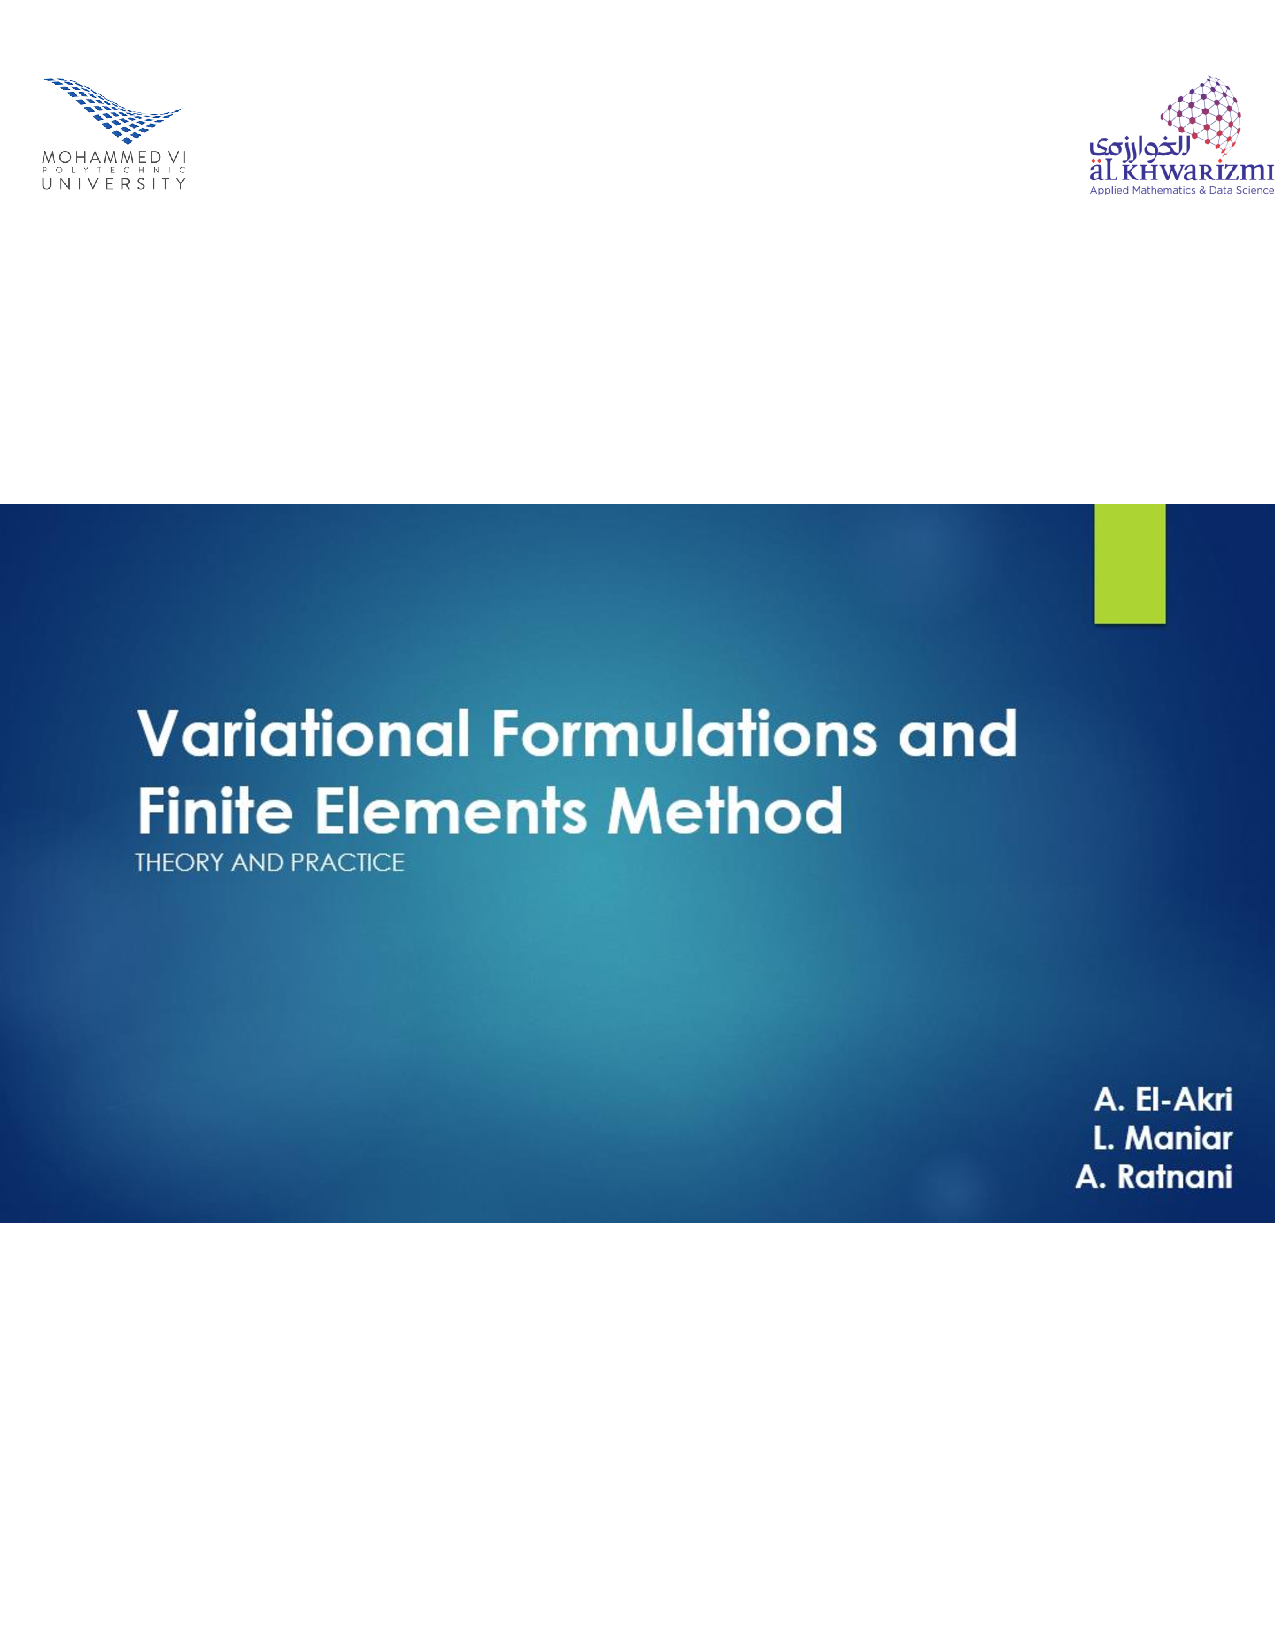
\includegraphics[width=\paperwidth]{titlepage-fem.pdf}};
\end{tikzpicture}
\vfill
\endgroup

%%----------------------------------------------------------------------------------------
%%	HALF TITLE PAGE
%%----------------------------------------------------------------------------------------
%
%\begingroup
%\newpage
%\thispagestyle{empty} % Suppress headers and footers on the title page
%\begin{tikzpicture}[remember picture,overlay]
%\node[inner sep=0pt] (background) at (current page.center) {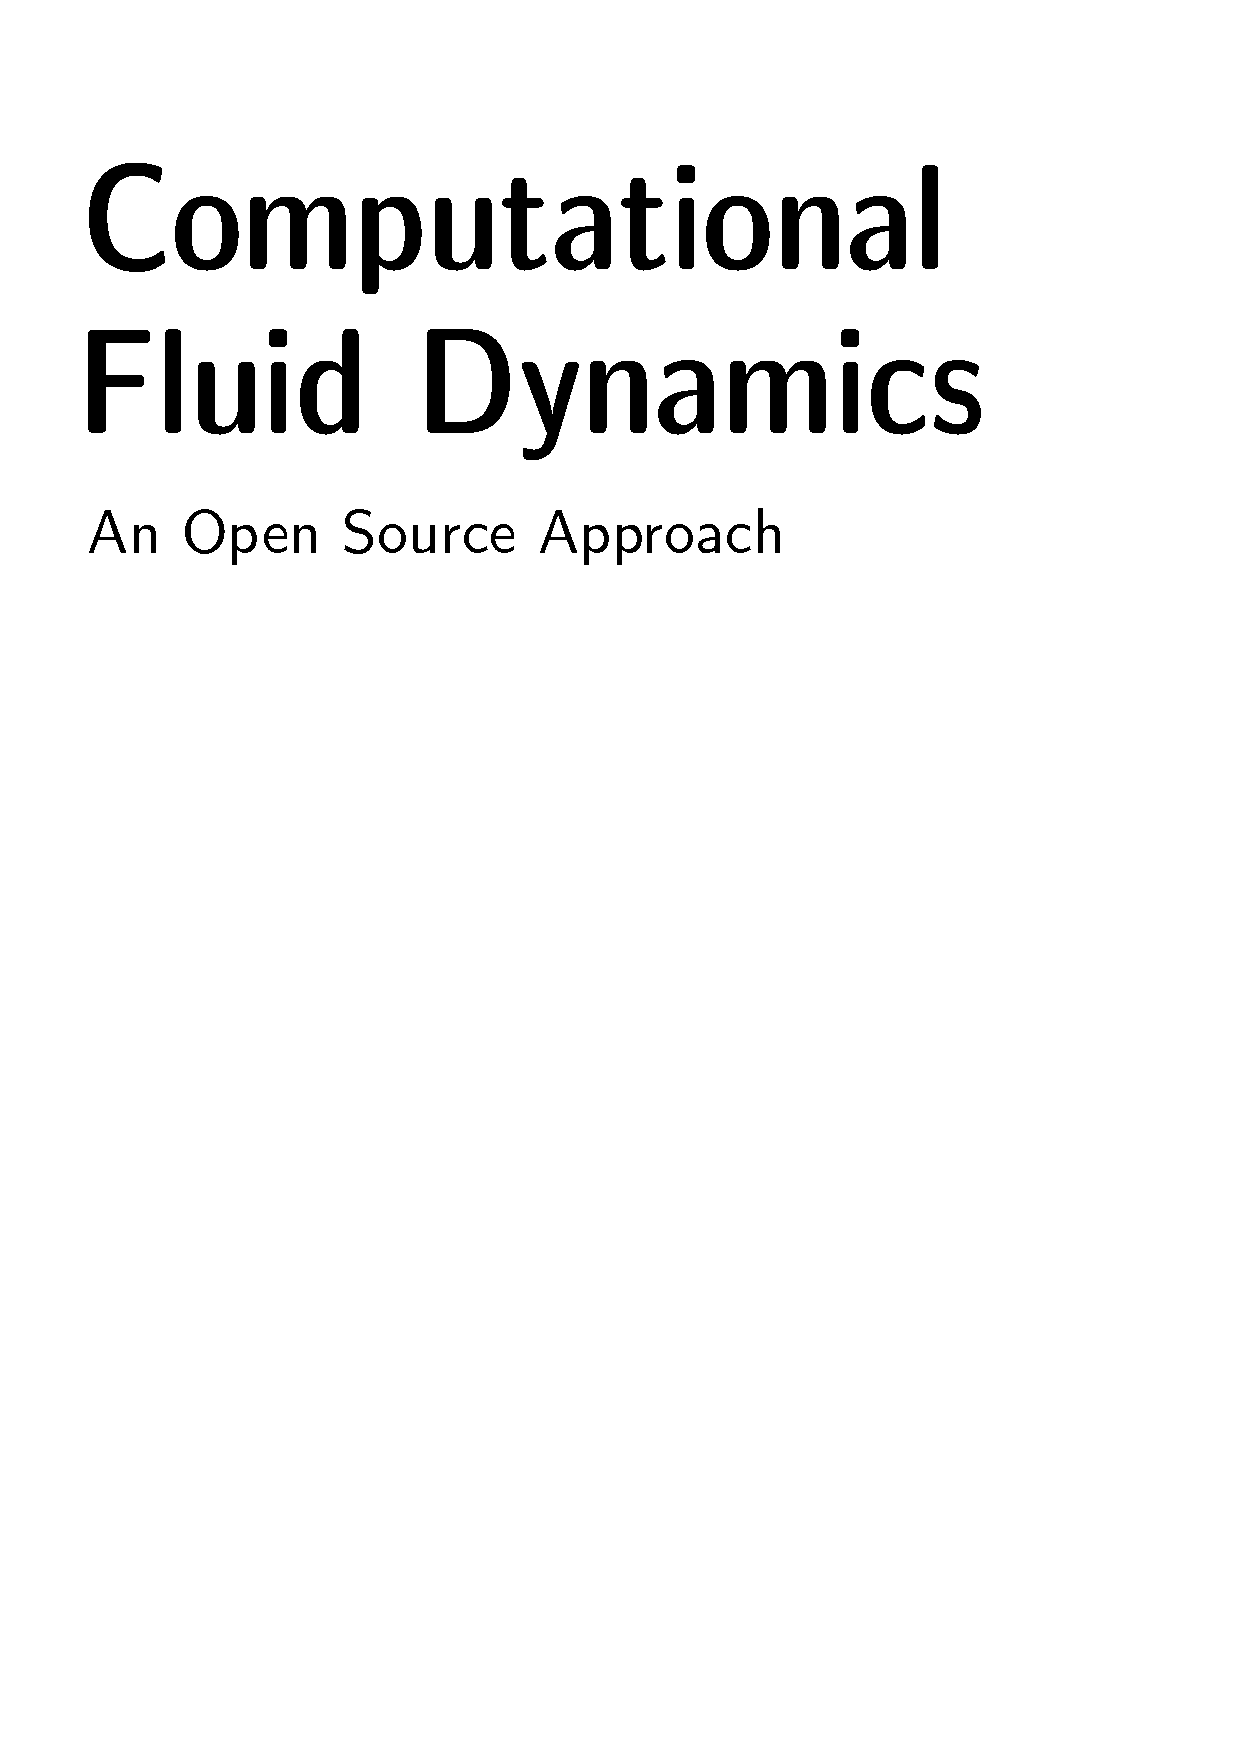
\includegraphics[width=\paperwidth]{halftitle.pdf}};
%\end{tikzpicture}
%\vfill
%\endgroup


%----------------------------------------------------------------------------------------
%	COPYRIGHT PAGE
%----------------------------------------------------------------------------------------

\newpage
~\vfill
\thispagestyle{empty}

\noindent Copyright \copyright\ 2021 AL-KHWARIZMI\\ % Copyright notice

\noindent \textsc{Published by UM6P University}\\ % Publisher

\noindent \textsc{um6p.ma}\\ % URL

\noindent Licensed under the Creative Commons Attribution-NonCommercial 3.0 Unported License (the ``License''). You may not use this file except in compliance with the License. You may obtain a copy of the License at \url{http://creativecommons.org/licenses/by-nc/3.0}. Unless required by applicable law or agreed to in writing, software distributed under the License is distributed on an \textsc{``as is'' basis, without warranties or conditions of any kind}, either express or implied. See the License for the specific language governing permissions and limitations under the License.\\ % License information, replace this with your own license (if any)

\noindent \textit{First printing, October 2021} % Printing/edition date

%----------------------------------------------------------------------------------------
%	FOREWORD
%----------------------------------------------------------------------------------------
\clearpage
\section*{Foreword}\index{Foreword}
TODO
%\vspace{0.5cm}
%
\noindent Abdeladim El-Akri 
\noindent Lahcen Maniar 
\noindent Ahmed Ratnani 



%----------------------------------------------------------------------------------------
%	TABLE OF CONTENTS
%----------------------------------------------------------------------------------------

\usechapterimagefalse % If you don't want to include a chapter image, use this to toggle images off - it can be enabled later with \usechapterimagetrue

\chapterimage{chapter_head_1.pdf} % Table of contents heading image

\pagestyle{empty} % Disable headers and footers for the following pages

\tableofcontents % Print the table of contents itself

\cleardoublepage % Forces the first chapter to start on an odd page so it's on the right side of the book

\pagestyle{fancy} % Enable headers and footers again

%----------------------------------------------------------------------------------------
%	PART 1: Functional Analysis 
%----------------------------------------------------------------------------------------
\part{Functional Analysis}
\chapter{Topology}
Dans ce chapitre, on s'intéresse à l'approximation numérique d'équations aux dérivées partielles linéaires qui admettent une formulation variationnelle. 

Exemple :  Considérons le problème suivant. 

Étant donné $f \in \mathrm{C}([a, b])$ trouver une fonction $u$ vérifiant
$$
(1)\;  \left\{\begin{array}{l}
	-u^{\prime \prime}+u=f \quad \text { sur } \quad]a, b[ \\
	u(a)=u(b)=0.
\end{array}\right.
$$
Une solution classique $-$ ou solution forte $-$ du problème (1) est une fonction de classe $\mathrm{C}^{2}$ sur $[a, b]$ vérifiant (1) au sens usuel. Bien entendu (1) peut être résolu explicitement par un calcul très simple, mais nous ignorerons cet aspect des choses afin d'illustrer la méthode sur cet exemple élémentaire.
On multiplie (1) par $\varphi \in C^{1}([a, b])$ et on intègre par parties; il vient
$$(2) \; \int_{a}^{b} u^{\prime} \varphi^{\prime}+\int_{a}^{b} u \varphi=\int_{a}^{b} f \varphi,    \qquad \forall \varphi \in \mathrm{C}^{1}([a, b]), \quad \varphi(a)=\varphi(b)=0.
$$
On notera que (2) a un sens dès que $u \in \mathrm{C}^{1}([a, b])$ (contrairement à (1) qui suppose $u$ deux fois dérivable); en fait il suffirait même d'avoir $u, u^{\prime} \in \mathrm{L}^{1}(a, b), u^{\prime}$, dérivée généralisée, ou dérivée au  un sens faible, voir plus loin. 

 Disons (provisoirement) qu'une fonction $u$ de classe $\mathrm{C}^{1}$ qui vérifie (2) est une solution faible de (1).

Le programme suivant décrit les grandes lignes de l'approche variationnelle en théorie des équations aux dérivées partielles :

Etape A. - On précise la notion de solution faible ; celle-ci fait intervenir les espaces de Sobolev qui sont les outils de base.

Etape B. - On établit l'existence et l'unicité d'une solution faible par la méthode variationnelle, via le théorème de Lax-Milgram.

Etape C. - On prouve quc la solution faible est de classe $\mathrm{C}^{2}$ (par exemple): c'est un résultat de régularité.


Etape D. - Retour aux solutions classiques. On montre qu'une solution faible de classe $\mathrm{C}^{2}$ est une solution classique.


L'équation (2),  peut être écrite sous la forme du problème "abstrait" général suivant :

$$
(PV) \text{ trouver } u \in W\;  \text{tel que } a(u, v)=L(v) \;\, \text{pour tout}\;\;  v \in V.
$$

 $W$ et  $V$ sont des espaces vectoriels normés. Dans plusieurs applications, $W$ and $V$ sont des espaces de Hilbert, mais  des cas où $V, W$ sont des  espace de  Banach  réflexifs  peuvent être considérés, $a:W\times V\longrightarrow \mathbb{R}$ une application bilinéaire continue
et $L$ une forme linéaire continue sur $V$, i.e. $L\in V'$. 

Ces formulations sont importantes pour les raisons suivantes :

1. De nombreux problèmes issus de la physique et de la mécanique admettent de telles formulations, et celles-ci reflètent souvent une propriété fondamentale du modèle, typiquement la minimisation d'une énergie sous-jacente.

2. Ces formulations donnent accès à des résultats fondamentaux sur le caractère bien posé de l'équation, c'est à dire l'existence et l'unicité de la solution, et la stabilité de cette solution par rapport à des perturbations des données.

3. Elles sont à la base de méthodes performantes pour l'approximation numérique des solutions, par la résolution d'un problème approché : 
\bigskip

\centerline{
trouver $u_{h} \in X_{h}$ tel que $a\left(u_{h}, v_{h}\right)=L\left(v_{h}\right)$ pour tout $v_{h} \in X_{h}$,} 

où $X_{h}$ est un sous-espace de dimension finie de $X$.

Le cours se concentre autour de ce dernier aspect qui pose la question du contrôle de l'erreur $u-u_{h}$ entre la solution exacte et la solution approchée. On s'interessera tout particulièrement à la méthode des éléments finis dans laquelle les fonctions de $X_{h}$ sont polynomiales par morceaux sur une partition du domaine de la solution de l'équation.


On définit quelques outils mathématiques nécessaires pour développer cette étude.

\section{Espaces Complets}


\subsection{ Normes et produits scalaires}
Soit $E$ un espace vectoriel.
\begin{definition}\
	
	$\|\cdot\|: E \rightarrow \mathbb{R}_{+}$ est une norme sur $E$ s'elle vérifie:
	
(N1) $\|x\|=0\Longrightarrow x=0$.

(N2) $\forall \lambda \in \mathbb{R}, \forall x \in E, \quad\|\lambda x\|=|\lambda|\|x\|$.

(N3) $\forall x, y \in E, \quad\|x+y\| \leq\|x\|+\|y\|$
(inégalité triangulaire).


- Un espace vectoriel muni d'une norme est appelé espace normé ou un evn.


\end{definition}
Exemples : 

1. Pour $E=\mathbb{R}^{n}$ et $x=\left(x_{1}, \ldots, x_{n}\right) \in \mathbb{R}^{n}$, on définit les normes
$$
\|x\|_{1}=\sum_{i=1}^{n}\left|x_{i}\right|,  \quad\|x\|_{2}=\left(\sum_{i=1}^{n} x_{i}^{2}\right)^{1 / 2},    \quad\|x\|_{\infty}=\sup _{i}\left|x_{i}\right|.
$$

2. Sur $E=\mathcal{C}([0,1], \R)$, le $\R$-espace vectoriel des fonction réelles continues sur $[0,1]$,  l'application 
$$
f\longmapsto\|f\|=\sup_{t\in[0,1]}|f(t)|
$$
est une  norme.



\begin{definition}\
	
On appelle produit scalaire sur $E$ toute forme bilinéaire symétrique définie positive : 

1. \; L'application $<\cdot, \cdot >: E \times E \rightarrow \mathbb{R}$ est donc un produit scalaire sur $E$ s'elle   vérifie :

(S1) $\forall x, y \in E, \quad\langle x, y\rangle =\langle y, x\rangle $.

(S2) $\forall x_{1}, x_{2}, y \in E, \quad\langle x_{1}+x_{2}, y\rangle =\langle x_{1}, y\rangle +\langle x_{2}, y\rangle $.

(S3) $\forall x, y \in E, \forall \lambda \in \mathbb{R}, \quad\langle \lambda x, y\rangle =\lambda\langle x, y\rangle $.

(S4) $\forall x \in E, x \neq 0, \quad\langle x, x\rangle >0$.


2.\; Un espace vectoriel $E$ muni d'un produit scalaire est appelé espace préhilbertien. 
\end{definition}

A partir d'un produit scalaire, on peut définir une norme induite: $\|x\|=\sqrt{\langle x, x\rangle}$.

 On a alors, d'après (N3), l'inégalité de Cauchy-Schwarz: $|\langle x, y\rangle | \leq\|x\|\|y\|$.

Exemple: 

Pour $E=\mathbb{R}^{n}$, on définit le produit scalaire $\langle x, y\rangle =\sum_{i=1}^{n} x_{i} y_{i} .$ 

Sa norme induite est $\|\cdot \|_{2}$ définie précédemment.

En général, si $E$ et $F$ sont deux evn, on peut définir l'espace produit 

$E\times F=\{ (x,y): x\in E, y\in F\}$, qui est un evn pour les normes 
$$
\|(x,y) \|_{1}= \|x \|_E+\|y \|_F,\quad  \|(x,y) \|_{2}= \sqrt{\|x \|_E^2+\|y \|_F^2}, \quad \|(x,y) \|_{\infty}=max(\|x \|_E,\|y \|_F). 
$$ 

Si $E$ et $F$ sont deux Hilbert, l'espace produit $E\times F$ est un Hilbert. 
\subsection{Suites de Cauchy : espaces et complets}

\begin{definition} \
	
1. 	\; Soit $E$ un espace vectoriel et $\left(x_{n}\right)_{n}$ une suite de $E $. $\left(x_{n}\right)_{n}$ est une suite de Cauchy ssi 
$$
\forall \varepsilon>0, \exists N >0 : \forall p>N, \forall q>N, \quad\left\|x_{p}-x_{q}\right\|<\varepsilon.
$$
	

2. \; Un espace vectoriel est complet si toute suite de Cauchy y est convergente.

3. \;  Un espace normé complet est un espace de Banach.

4. \; Un espace préhilbertien complet est un espace de Hilbert.

5. \;  Un espace de Hilbert de dimension finie est appelé espace euclidien.

\end{definition}


\subsection{Espaces fonctionnels}
\begin{definition}
	
Un espace fonctionnel est un espace vectoriel dont les éléments sont des fonctions.

\end{definition} 


Exemples :

1. L'espace des fonctions continues sur un intervale $[a, b]$ à valeurs réelles, noté $\mathcal{C}^{0}([a ; b])$ ou juste $\mathcal{C}([a ; b])$.   $\mathcal{C}([a ; b])$ muni de la norme $\|f\|_{\infty}= \sup_{[a, b]} |f(x)|$ est un espace complet (Banach).

2.  $\mathcal{C}^{p}([a ; b])$ désigne l'espace des fonctions définies sur l'intervalle $[a, b]$ à valeurs dans $\mathbb{R}$, dont toutes les dérivées jusqu'à l'ordre $p$ existent et sont continues sur $[a, b]$.

Dans la suite, les fonctions seront définies sur un sous-ensemble de $\mathbb{R}^{n}$ (le plus souvent un ouvert noté $\Omega$ ), à valeurs dans $\mathbb{R}$ ou $\mathbb{R}^{m}$.

Exemple: La température $T(x, y, z, t)$ en tout point d'un objet $\Omega \subset \mathbb{R}^{3}$ est une fonction de $\Omega \times \mathbb{R} \longrightarrow \mathbb{R}$.

Les normes usuelles les plus simples sur les espaces fonctionnels sont les normes $L^p$  définies par :
$$
\|u\|_{L^p}=\left(\int_{\Omega}|u(x)|^{p}\right)^{1 / p},  \quad p \in[1,+\infty[, \quad \text{ et } \quad\|u\|_{L^{\infty}}= \sup_{\Omega} |u(x)|. 
$$

Ces applications  ne sont pas nécessairement des normes; et lorsqu'elles le sont, les espaces fonctionnels munis de ces normes ne sont pas nécessairement des espaces de Banach. Par exemple, les applications  $\|\cdot \|_{L^1}, \|\cdot \|_{L^{\infty}}$  sont bien des normes sur l'espace $\mathcal{C}^{0}([a ; b])$, et cet espace est complet si on le munit de la norme $\|\cdot \|_{L^{\infty}}$, mais ne l'est pas si on le munit de la norme $\|\cdot \|_{L^1}$.

Pour cette raison, on va définir les espaces $\mathcal{L}^{p}(\Omega)(p \in[1,+\infty[)$ par
$$
\mathcal{L}^{p}(\Omega)=\left\{u: \Omega \rightarrow \mathbb{R}, \text { mesurable, et telle que } \int_{\Omega}|u|^{p}<\infty\right\}.
$$
(on rappelle qu'une fonction $u$ est mesurable ssi $\{x \in \Omega /|u(x)|<r\}$ est mesurable dans $\mathbb{R}^n$,  pour tout $ r>0$. )

Sur ces espaces $\mathcal{L}^{p}(\Omega)$, les applications  $\|\cdot \|_{L^p}$ ne sont pas des normes. En effet, 

$\|u\|_{L^{p}}=0$ implique que $u$ est nulle presque partout dans $\mathcal{L}^{p}(\Omega)$, et non pas $u=0$. 

C'est pourquoi on va définir les espaces $L^p(\Omega)$ :

\begin{definition}\
	
L'espace  $L^{p}(\Omega), p\geq 1,$ est l'ensemble des classes d'équivalence des fonctions de $\mathcal{L}^{p}(\Omega)$ pour la relation d'équivalence "égalité presque partout". Autrement dit, on confondra deux fonctions dès lors qu'elles sont égales presque partout, c'est à dire qu'elles ne different que sur un ensemble de mesure nulle.

\end{definition}

\begin{theorem}\
	
L'application  $\|\cdot \|_{L^p}$ est une norme sur $L^{p}(\Omega)$, et $L^{p}(\Omega)$ muni de cette  norme  est un espace de Banach.

Pour  $p=2$,   l'espace fonctionnel $L^{2}(\Omega)$,  des fonctions de carré sommable sur $\Omega$, la norme $\|\cdot \|_{L^{2}}$, est la norme induite  du produit scalaire $$<u, v>_{L^{2}}=\int_{\Omega} u v dx,
$$

 et donc   $L^{2}(\Omega)$ est un espace de Hilbert.
 
 On défint aussi l'espace $L^\infty(\Omega)$ par 
 
 $$
 \mathrm{L}^{\infty}(\Omega)=\{f: \quad \Omega \rightarrow \mathbb{R} ; f \; \text{mesurable et } \, \exists  \mathrm{C}>0 :  |f(x)| \leq \mathrm{C} \; \text{ p.p. sur } \Omega\}
 $$
 
 L'application 
 $$
 \|f\|_{L^{\infty}}= \sup_{\Omega} |f(x)|
 $$

est une norme sur $L^\infty(\Omega)$ et  $(L^\infty(\Omega), \|\cdot \|_{L^{\infty}})$ est un espace de Banach.

\end{theorem}

\section{Dual Topologique}

Soit $V$ un espace de Banach (un $\mathbb{K}$-espace vectoriel),  muni d'une norme $\|\cdot \|_V$.  Le dual topologique de $V$ est l'ensemble des applications linéaires continues de $V$ dans $\mathbb{K}$,  noté $V'$. Donc, $V'=\mathcal{L}_c(V,\mathbb{K}),, \mathcal{L}(V,\mathbb{K})$ est un espace de Banach pour la norme 
$$
\displaystyle\|f \|=\sup_{v\in V,v\neq0}\frac{|f(v) |}{\|v\|_V} \quad = \sup_{v\in V,\|v\|_V\leq 1}|f(v) |, 
$$  

pour $f\in V'$.  Les éléments de $V'$ sont dites des formes linéaires de $V$. 

Pour un espace de Hilbert $H$, on a $H'=H$. On identifie $H$ et son dual topologique 

(via une isométrie, Théorème de représentation de  Riesz). 

Un espcace de Banach $X$, est dit réflexif si $X^{\prime\prime}=X$.  

Exemple :  Soit $p>1$, l'espace dual de $L^p(\Omega)$ est  l'espace $L^q(\Omega)$, avec $\frac1p+\frac1q=1$.  

En particulier, pour $p=2$, $q=2$ ($\frac12+\frac12=1$) et  donc $(L^2(\Omega))^\prime=L^2(\Omega)$, 

c'est normal puisque c'est un Hilbert.

Pour $p=1$,  $(L^1(\Omega))^\prime=L^\infty(\Omega)$. 

Pour $p>1$, l'espace $L^p(\Omega)$ est un Banach réflexif.   En effet ...

\begin{remark}\
	
1. Si $V$ et $H$ sont deux espaces de Hilbert tels que $V\subset H$.   On identifie $H$ avec son dual $H'$, mais pas $V$ et on a 
$$
	V\subset H=H'\subset V',
	$$
	
	car, en général,  si $V$ et $W$  sont deux Banach tel que $V\subset W$ alors $W'\subset V'$.  
	
	On dit que $V'$ est le dual de $V$ par rapport au pivot $H$.


Exemple (exercice):	 Soient les epaces 
$$
\begin{aligned}
	&H=l^{2}=\left\{u=\left(u_{n}\right) ; \sum u_{n}^{2}<\infty\right\}  \text { muni du produit scalaire }\langle u, v\rangle=\sum u_{n} v_{n} \\
	&V=\left\{u=\left(u_{n}\right) ; \Sigma n^{2} u_{n}^{2}<\infty\right\} \text { muni du produit scalaire }\langle \langle u, v\rangle\rangle=\sum n^{2} u_{n} v_{n}
\end{aligned}
$$

Calculer $V'$. 


2.  Pour un $\phi\in V'$,   et $v\in V$, on note $\phi(v)=\langle \phi, v\rangle_{V^{\prime}, V}$, qu'on appelle  le crochet de dualité entre $V$ et $V'$. Ce crochet est identifié au produit scalaire dans le cas d'un Hiblbert $H$  tel que $H=H'$.

\end{remark} 

\section{Problems}

\begin{exercise}
  TODO
\end{exercise}


\chapter{Introduction to Functional Analysis}
\section{Dérivée généralisée et Espaces de Sobolev}
Nous venons de définir des espaces fonctionnels complets, ce qui sera un bon cadre pour démontrer l'existence et l'unicité de solutions d'équations aux dérivées partielles, comme on le verra plus loin notamment avec le théorème de Lax-Milgram. Toutefois, on a vu que les éléments de ces espaces $L^{p}$ ne sont pas nécessairement des fonctions très régulières. Dès lors, les dérivées partielles de telles fonctions ne sont pas forcément définies partout. Pour s'affranchir de ce problème, on va étendre la notion de dérivation à  la notion  de dérivée généralisée.  Ceci  pertmettra d'introduire de nouveux espaces fonctionnels, sous espaces des $L^p$, analogue aux espaces $C^p(\Omega)$.  

Dans la suite, $\Omega$ sera un ouvert (pas nécessairement borné) de $\mathbb{R}^{n}$.

\subsection{Fonctions tests} 

\begin{definition}\
	
	
	Soit $\varphi: \Omega \rightarrow \mathbb{R}$. On appelle support de $\varphi$ l'adhérence de $\{x \in \Omega :  \varphi(x) \neq 0\}$. 
	
	On le note $supp(\varphi)$. 
	\end{definition}
Exemple : Pour $\Omega=]-1,1[$, et $\varphi$ la fonction constante égale à 1, $supp(\varphi)=[-1,1]$.

\begin{definition}\
	
On note $\mathcal{D}(\Omega)$ l'espace des fonctions de $\Omega$ vers $\mathbb{R}$, de classe $\mathcal{C}^{\infty}$, et à support
compact inclus dans $\Omega.$  $ \mathcal{D}(\Omega)$ est parfois appelé espace des fonctions-tests.

\end{definition}

Exemple: L'exemple le plus classique dans le cas de $\mathbb{R}$ est la fonction.
$$
\varphi(x)= \begin{cases}e^{-\frac{1}{1-x^{2}}} & \text { si }|x|<1 \\ 0 & \text { si }|x| \geq 1\end{cases}
$$
$\varphi$ est une fonction de $\mathcal{D}( ]-1, 1[ )$  et $supp(\varphi)=[-1,1]$.

\begin{theorem}\
	
$\overline{\mathcal{D}(\Omega)}=L^{p}(\Omega)$, $1\leq p\leq \infty$,  i.e. $\mathcal{D}(\Omega)$ est dense dans $L^{p}(\Omega)$ : pour tout $f\in L^{p}(\Omega)$, il existe une suite $(f_n)\subset \mathcal{D}(\Omega)$ convergente vers $f$.
\end{theorem}


\subsection{Dérivée généralisée}
On définit une notion de dérivée pour des fonctions qui ne sont pas  nécessairement de classe $\mathcal{C}^{1}$. 

\begin{definition}\ 
	
Soit $I$ un intervalle de $\mathbb{R}$, pas forcément borné. On dit que $u \in L^{2}(I)$ admet une dérivée généralisée dans $L^{2}(I)$ si 
 
 $$\exists u_{1} \in L^{2}(I) :  \forall \varphi \in \mathcal{D}(I), \quad \int_{I} u \varphi^{\prime}=-\int_{I} u_{1} \varphi .
 $$ 
 
La fonction $u_1$ est unique dans  $ L^{2}(I)$, et elle est dite la dérivée généralisée, dérivée au sens des distributions, ou dérivée au sens faible, de $u$. On la note aussi $u_1=u'$.
 
 En itérant, on dit que $u$ admet une dérivée généralisée d'ordre $k$ dans
 $L^{2}(I)$, notée $u_{k}$, si $$\forall \varphi \in \mathcal{D}(I), \quad \int_{I} u_{k} \varphi=(-1)^{k} \int_{I} u \varphi^{(k)}.
 $$
 
 On note aussi $u_k=u^{(k)}$, la $k$-ème dérivée de $u$. 
 
 Ces définitions s'étendent naturellement pour la définition de dérivés partielles généralisées du premier ordre, notées $\partial_{i}, \partial_{x_i}, $ ou $\frac{\partial}{\partial x_i}$, $ i=1, \dots, n$,  dans le cas multidimension (dans $\mathbb{R}^n, n>1$) et aussi pour les dérivés partielles généralisées d'ordre supérieur ($m\geq 2$), notées $\partial^\alpha$, ou $\frac{\partial^{\alpha_{1}}}{\partial x_{1}^{\alpha_{1}}} \frac{\partial^{\alpha_{2}}}{\partial x_{2}^{\alpha_{2}}} \cdots \frac{\partial^{\alpha_{N}}}{\partial x_{n}^{\alpha_{n}}}$, pour $\alpha =(\alpha_1, \cdots, \alpha_n)$ tel que $|\alpha|=\alpha_{1}+\cdots+\alpha_{n} =m$. 
 
\end{definition}

Exemple : 

Soit $I=] a, b[$ un intervalle borné, et $c$ un point de $I$. On considère une fonction $u$ formée de deux branches de classe $\mathcal{C}^{1}$,  l'une sur $] a, c[$,  l'autre sur 
$] c, b[$ et se raccordant de  façon continue mais non dérivable en $c$. Alors $u$ admet une dérivée généralisée définie par $u_{1}(x)=u^{\prime}(x),   \quad \forall x \neq c$. 
 En effet :
\begin{align*}
	\forall \varphi \in \mathcal{D}(]a, b[),  \quad \int_{a}^{b} u \varphi^{\prime}&=\int_{a}^{c}u \varphi^{\prime}+\int_{c}^{b}u \varphi^{\prime}\\
	&=-\int_{a}^{c} u^{\prime} \varphi-\int_{c}^{b} u^{\prime} \varphi+\underbrace{\left(u\left(c^{-}\right)-u\left(c^{+}\right)\right)}_{=0} \varphi(c)\\
	&=-\int_{a}^{b} u^{\prime} \varphi.
\end{align*}

Donc, $u_1=u'$ est la dérivée généralisée de $u$. 
 La valeur $u_{1}(c)$ n'a pas d'importance: on a de toute façon au final la même fonction de $L^{2}(I)$, puisqu'elle est définie comme classe d'equivalence de la relation d'équivalence "égalité presque partout".

Un autre espace de fonctions régulières qui joue un rôle important par la suite est  
$$
\mathcal{C}^{1}(\bar{\Omega})=\left\{\varphi: \Omega \rightarrow \mathbb{R} : \exists \; O \; \text { ouvert contenant } \bar{\Omega}, \exists \psi \in \mathcal{C}^{1}(O), \psi_{\mid \Omega}=\varphi\right\}
$$

Autrement dit, $\mathcal{C}^{1}(\bar{\Omega})$ est l'espace des fonctions $\mathcal{C}^{1}$ sur $\Omega$, prolongeables par continuité sur $\partial \Omega$ et dont le gradient est lui-aussi prolongeable par continuité. 


\begin{theorem}\
	
1. 	 Quand elle existe, la dérivée généralisée est unique.

 2. Quand $u$ appartient  à $\mathcal{C}^{1}(\bar{\Omega})$, les dérivées généralisées sont  égales  aux  dérivées classiques.
\end{theorem}

\subsection{Espaces de Sobolev}

Dans cette sous-section,  on introduit  de nouveaux espaces fonctionnels, sous espaces des espaces  $L^p$, analogue aux espaces $C^p(\Omega)$, $p\geq 1$.   On commence par  $p=2$, le  cas le plus  utilisé. 
\subsubsection{Les espaces $H^{m}$}

\begin{definition}\
	
1. 	L'espace de Sobolev d'ordre $1 $  dans  $L^{2}(\Omega)$  est l'ensemble défini par
$$
H^{1}(\Omega)=\left\{u \in L^{2}(\Omega) : \partial_{i} u \in L^{2}(\Omega), \quad 1 \leq i \leq n\right\},
$$ 

où $\partial_{i} u$ est définie au sens de la dérivée généralisée. 

 2. Pour tout entier $m \geq 1$, le sous ensemble de $L^{2}(\Omega)$
$$
H^{m}(\Omega)=\left\{u \in L^{2}(\Omega): \partial^{\alpha} u \in L^{2}(\Omega),  \forall \alpha=\left(\alpha_{1}, \ldots, \alpha_{n}\right) \in \mathbb{N}^{n}: |\alpha|=\alpha_{1}+\cdots+\alpha_{n} \leq m\right\}
$$

est appelé espace de Sobolev d'ordre $m$.

3. Par extension, on voit aussi que $H^{0}(\Omega)=L^{2}(\Omega)$.

4. Dans le cas de la dimension 1, on écrit plus simplement pour $I$ ouvert de $\mathbb{R}$ :
$$
H^{m}(I)=\left\{u \in L^{2}(I) :  u^{\prime}, \ldots, u^{(m)} \in L^{2}(I)\right\}.
$$

\end{definition}

Exemple :  (exercice)  

Soient $\mathrm{I}=]-1,+1[ $ et  la fonction $u(x)=\frac{1}{2}(|x|+x)$. 

1. Montrer  que $u$  appartient à $H^1(\mathrm{I})$  et que $u^{\prime}=\mathrm{H}$ où
$$
\mathrm{H}(x)=\left\{\begin{array}{clrl}
	+1 & \text { si } & 0<x<1 \\
	0 & \text { si } & -1<x<0.
\end{array}\right.
$$

2. Montrer que $H$ n'appartient pas à $H^1(\mathrm{I})$. 
\begin{theorem}\
	
1. 	$H^{1}(\Omega)$ est un espace de Hilbert pour le produit scalaire
\begin{equation}\label{H1}
	\langle u, v\rangle_{1}=\int_{\Omega} u v+\sum_{i=1}^{n} \int_{\Omega} \partial_{i} u \partial_{i} v=\langle u, v\rangle+\sum_{i=1}^{n}\langle\partial_{i} u, \partial_{i} v\rangle, 
\end{equation}

en notant $\langle\cdot, \cdot \rangle$ le produit scalaire $L^{2}$. On notera $\|\cdot\|_{1}$ la norme associée à $\langle \cdot, \cdot\rangle_{1}$.


2. 
Si $\Omega$ est un ouvert de $\mathbb{R}^{n}$ de frontière $\partial \Omega$ "suffisamment régulière" (par exemple
$\left.\mathcal{C}^{1}\right)$,  l'espace $\mathcal{C}^{1}(\bar{\Omega})$ est dense dans $H^{1}(\Omega)$. 



3. On définit de même un produit scalaire et une norme sur $H^{m}(\Omega)$ par
$$
\langle u, v\rangle_{m}=\sum_{|\alpha| \leq m}\langle \partial^{\alpha} u, \partial^{\alpha}v\rangle  \qquad \text { et } \quad\|u\|_{m}=(u, u)_{m}^{1 / 2}
$$

$H^{m}(\Omega)$ muni du produit scalaire $\langle u, v\rangle_{m}$ est un espace de Hilbert.

4.  Si $\Omega$ est un ouvert de $\mathbb{R}^{n}$ de frontière $\partial \Omega$ "suffisamment régulière" (par exemple
$\left.\mathcal{C}^{1}\right)$, on a l'inclusion: $H^{\mathrm{m}}(\Omega) \subset \mathcal{C}^{k}(\Omega)$ (injection continue) pour $k<m-\frac{n}{2}$.


\end{theorem}
Exemples: En particulier, on voit que pour un intervalle $I$ de $\mathbb{R}$, on a $H^{1}(I) \subset \mathcal{C}^{0}(I)$, c'est à dire que, en 1-D, toute fonction $H^{1}$ est continue.

L'exemple de $u(x)=x \sin \frac{1}{x}$ pour $\left.\left.x \in\right] 0,1\right]$ et $u(0)=0$ montre que la réciproque est fausse.  (Exercice).


L'exemple de $u(x, y)=\left|\ln \left(x^{2}+y^{2}\right)\right|^{k}$ pour $0<k<1 / 2$ montre qu'en dimension supérieure à $1$,  il existe des fonctions $H^{1}$ discontinues. (Exercice).


Les fonctions de $H^{1}$ sont « en gros » des primitives de fonctions de $L^{2}$. Plus précisément on a le résultat suivant :

\begin{theorem}
	
 Soit $u \in H^{1}(I) ;$ alors il existe une fonction $\tilde{u} \in \mathrm{C}(\bar{I})$ telle que et
$$
\begin{aligned}
	\boldsymbol{u} &=\tilde{\boldsymbol{u}}\;\;  \text { p.p. sur } \mathbf{I} \\
	\tilde{\boldsymbol{u}}(\boldsymbol{x})-\tilde{\boldsymbol{u}}(y) &=\int_{y}^{x} \boldsymbol{u}^{\prime}(\boldsymbol{t}) \mathrm{d} t,     \quad \forall x, y \in \overline{\mathrm{I}}.
\end{aligned}
$$

\end{theorem}


Pour $1 \leqslant p \leqslant \infty$,  on peut définir aussi les espaces de Sobolev suivants:


L'espace de Sobolev $\mathbf{W}^{1, p}(\Omega)$ est défini par $\left({ }^{1}\right.$ )
$$
\mathbf{W}^{1, p}(\Omega)=
\left\{u \in \mathrm{L}^{p}(\Omega) : 
	\exists  g_{1}, g_{2}, \dots, g_n\in \mathrm{L}^{p}(\Omega) :
	\int_{\Omega}u \frac{\partial \varphi}{\partial x_i}=-\int_{\Omega} g_{i} \varphi \quad \forall \varphi \in D(\Omega),  \quad \forall i=1,2, \dots,n. 
\right\}
$$

Pour $p=2$, 
$\mathrm{W}^{1,2}(\Omega)= \mathrm{H}^{1}(\Omega)$. 

Pour $u\in \mathrm{W}^{1,p}(\Omega)$, $ g_{i}=\frac{\partial u}{\partial x_{i}}$ est la dérivée généralisée de $u$.  On note 

$$
 \nabla u=\left(\frac{\partial u}{\partial x_{1}}, \frac{\partial u}{\partial x_{2}}, \cdots, \frac{\partial u}{\partial x_{\mathrm{N}}}\right)=\operatorname{grad} u
$$
le gradient généralisé. 

L'espace $\mathbf{W}^{1, p}(\Omega)$,  muni de la norme
$$
\|u\|_{\mathrm{W}^{1, p}}=\|u\|_{\mathrm{L}^p}+\sum_{i=1}^{\mathrm{N}}\left\|\frac{\partial u}{\partial x_{i}}\right\|_{\mathrm{L}^p}
$$

ou parfois de la norme équivalente $\left(\|u\|_{L^{p}}^{p}+\displaystyle \sum_{i=1}^{N}\left\|\frac{\partial u}{\partial x_{i}}\right\|_{L^{P}}^{p}\right)^{1 / p}$ (si $\left.1 \leqslant p<\infty\right)$,

est un Banach. 

Si  $\Omega$ est borné, alors  $C^{1}(\bar{\Omega}) \subset \mathbf{W}^{1, p}(\Omega)$  pour tout  $1 \leqslant p \leqslant \alpha$.


\subsection{Trace d'une fonction}

Pour pouvoir faire les intégrations par parties qui seront utiles par exemple pour la formulation variationnelle, il faut pouvoir définir le prolongement (la trace) d'une fonction sur le bord $\partial \Omega$ de l'ouvert $\Omega$.

Si $n=1$ : on considère un intervalle ouvert $I=] a, b[$ borné. On a vu que $H^{1}(I) \subset$ $\mathcal{C}^{0}(\bar{I})$ . Donc, pour  $u \in H^{1}(I), u$ est continue sur $[a, b]$. La  trace (la valeur )  de $u$,  sur les bords $a$ et $b$ de l'intervalle  $I=] a, b[$, $u(a), u(b)$,  est  bien définie.


$\underline{\text { Si }} n>1$ : on n'a plus $H^{1}(\Omega) \subset \mathcal{C}^{0}(\bar{\Omega})$. Comment alors définir la trace d'une fonction $u\in H^{1}(\Omega)$ sur le bord $\partial \Omega$ ?  La démarche est la suivante :

- Pour une fonction $u\in 
\mathcal{C}^{1}(\bar{\Omega})$,  la trace de $u$ sur $\partial \Omega$, notée $u|_{\partial \Omega}$,  est  bien définie. 

- On peut voir que l'application linéaire  $\gamma_0: \mathcal{C}^{1}(\bar{\Omega})\ni u \longmapsto u|_{\partial \Omega}$ est  continue. 

- Comme, si $\Omega$ est un ouvert borné de frontière $\partial \Omega$ "assez régulière", alors $\mathcal{C}^{1}(\bar{\Omega})$ est dense dans $H^{1}(\Omega)$, alors, on a : le théorème trace: 

$\gamma_0$  se prolonge en une application linéaire continue de $H^{1}(\Omega)$ dans $L^{2}(\partial \Omega)$, notée encore 

$\gamma_{0}$, qu'on appelle opérateur  trace ($\gamma_{0}(u)$ est la trace de $u$ sur $\partial \Omega$). 

Pour une fonction $u$ de $H^{1}(\Omega)$ qui soit en même temps continue sur $\bar{\Omega}$, on a évidemment 

$\gamma_{0}(u)=u_{\mid \partial \Omega} .$ C'est pourquoi on note souvent par abus simplement $u_{\mid \partial \Omega}$ plutôt que $\gamma_{0}(u)$.

%
%On peut de façon analogue définir $\gamma_{1}$, application trace qui permet de prolonger la définition usuelle de la dérivée normale sur $\partial \Omega$. Pour $u \in H^{2}(\Omega)$, on a $\partial_{i} u \in H^{1}(\Omega), \forall i=1, \ldots, n$, et on peut donc définir $\gamma_{0}\left(\partial_{i} u\right)$. La frontière $\partial \Omega$ étant "assez régulière" (par exemple, idéalement, de classe $\left.\mathcal{C}^{1}\right)$, on peut définir la normale $n=\left(\begin{array}{l}n_{1} \\ \vdots \\ n_{n}\end{array}\right)$ en tout point de $\partial \Omega$. On pose alors $\gamma_{1}(u)=\sum_{i=1}^{n} \gamma_{0}\left(\partial_{i} u\right) n_{i}$. Cette application continue $\gamma_{1}$ de $H^{2}(\Omega)$ dans $L^{2}(\partial \Omega)$ permet donc bien de prolonger la définition usuelle de la dérivée normale. Dans le cas où $u$ est une fonction de $H^{2}(\Omega)$ qui soit en même temps dans $\mathcal{C}^{1}(\bar{\Omega})$, la dérivée normale au sens usuel de $u$ existe,

La formule de Green suivante généralise la notion d'intégration par parties. 
\begin{proposition}Formule de Green.\
	
	 On suppose que $\Omega$ est borné et de classe $C^{1}$. Soit $u, v \in H^{1}(\Omega) .$ Alors, 
	 
	  pour tout $i=1, \ldots, d$,  on a
$$
\int_{\Omega} \frac{\partial u}{\partial x_{i}} v d x=-\int_{\Omega} u \frac{\partial v}{\partial x_{i}} d x+\int_{\partial \Omega} u v n_{i} d \sigma
$$
où $n_{i}$ désigne la i-ème composante de la normale extérieure unitaire $\vec{n}$ à $\partial \Omega$.

Cette formule généralise la formule d'intégrations par parties sur $\mathbb{R}$ :

$$
\int_{a}^b u^\prime v d x=-\int_{a}^b u v^\prime d x+u(b)v(b)-u(a)v(a).
$$
\end{proposition}
\subsection{ Espace $\mathrm{H}_{0}^{1}(\Omega)$}

\begin{definition}\
	
 Soit $\Omega$ un ouvert de $\mathbb{R}^{n}$. L'espace $H_{0}^{1}(\Omega)$ est défini comme l'adhérence de $\mathcal{D}(\Omega)$ pour la norme $\|\cdot\|_{1}$ de $H^{1}(\Omega) .$ 

\end{definition}
\begin{theorem}\
	
Par construction $H_{0}^{1}(\Omega)$ est un espace complet. C'est un espace de Hilbert pour le produit scalaire de $H^1(\Omega)$. 
	
Si $n=1$ (cas 1-D) : on considère un intervalle ouvert $I=] a, b[$ borné. Alors
$$
H_{0}^{1}(] a, b[)=\left\{u \in H^{1}(] a, b[), u(a)=u(b)=0\right\}.
$$

Si $n>1:$ Si $\Omega$ est un ouvert borné de frontière "assez régulière" 

(par exemple $\mathcal{C}^{1}$ par morceaux, alors $H_{0}^{1}(\Omega)=\operatorname{ker} \gamma_{0}$.  

D'où, comme dans le cas $n=1$,  pour $u\in H^{1}(\Omega)$, $u\in H_{0}^{1}(\Omega)$ ssi   $\gamma_0u=0$.

\end{theorem}

 Pour toute fonction $u$ de $H^{1}(\Omega)$,  on peut définir l'application:
$$
|u|_{1}=\left(\sum_{i=1}^{n}\left\|\partial_{i} u\right\|_{L^2}^{2}\right)^{1 / 2}=\left(\int_{\Omega} \sum_{i=1}^{n}\left(\partial_{i} u\right)^{2} d x\right)^{1 }=\|\nabla u\|_{L^2} .
$$


\begin{theorem}(Inégalité de Poincaré) \
	
	Si $\Omega$ est borné, alors il existe une constante $C(\Omega)$ telle que 
	$$
	\forall u \in H_{0}^{1}(\Omega),\|u\|_{L^2} \leq C(\Omega)\|\nabla u\|_{L^2} .
	$$
	
On en déduit que $|\cdot|_{1}$ est une norme sur $H_{0}^{1}(\Omega)$, équivalente à la norme $\|\cdot\|_{1}$.


\end{theorem}

Dans la suite, on pourra avoir besoin du dual topologique  de $H_{0}^{1}(\Omega)$ qu'on note $H^{-1}(\Omega)$. On a ce résultat plus concret 


\begin{proposition}
	
	L'espace $H^{-1}(\Omega)$  est caractérisé par 
$$
H^{-1}(\Omega)=\left\{f=v_{0}+\sum_{i=1}^{n} \frac{\partial v_{i}}{\partial x_{i}} \quad \text { with } v_{0}, v_{1}, \ldots, v_{n} \in L^{2}(\Omega)\right\}
$$
Autrement, toute forme linéaire sur  $H_{0}^{1}(\Omega)$,  notée  $L \in H^{-1}(\Omega)$, est écrite  pour tout  $\phi \in H_{0}^{1}(\Omega)$
$$
L(\phi)=\int_{\Omega}\left(v_{0} \phi-\sum_{i=1}^{n} v_{i} \frac{\partial \phi}{\partial x_{i}}\right) d x
$$

avec  $v_{0}, v_{1}, \ldots, v_{n} \in L^{2}(\Omega)$.

Pour  $v \in L^{2}(\Omega) .$ For $1 \leq i \leq N$,  on définit forme linéaire  continue, dit dérivée faible au sens de $L^2$,  $\frac{\partial v}{\partial x_{i}}$ dans  $H^{-1}(\Omega)$ par 
$$
\left\langle\frac{\partial v}{\partial x_{i}}, \phi\right\rangle_{H^{-1}, H_{0}^{1}(\Omega)}=-\int_{\Omega} v \frac{\partial \phi}{\partial x_{i}} d x \quad \forall \phi \in H_{0}^{1}(\Omega).
$$

$\langle\cdot, \cdot \rangle_{H^{-1}, H_{0}^{1}}$ est   le crochet de dualité entre $H^{-1}$ et $H_{0}^{1}$.  On a le résultat : $$H_{0}^{1}(\Omega) \subset L^{2}(\Omega) \equiv\left(L^{2}(\Omega)\right)^{\prime} \subset H^{-1}(\Omega).
$$

\end{proposition}

Pour $1\leq p\leq \infty$, par la même technique, on peut aussi  définir les espaces  $W^{1,p}_0$, les fonctions de $W^{1,p}$ de traces nulles. 

\subsection{Dérivée Normale}

\begin{definition}
	
Pour $u \in H^{2}(\Omega)$, sa dérivée normale sur $\Gamma$ est définie par
$$
\gamma_{0} \frac{\partial u}{\partial \nu}=\sum_{i=1}^{n} \nu_{i} \gamma_{0} \frac{\partial u}{\partial x_{i}}
$$

où $\nu_{i}(x)$ désigne la ieme composante de la fonction $\nu(x)$,  le vecteur normal (perpendiculaire à la tengente au point $x\in \partial \Omega$. On note parfois cette dérivée normale par  $\gamma_1$, ou juste $\partial_n u$, ou $\frac{\partial u}{\partial n}$. 

\end{definition}


Remarquons que $\gamma_{0} \frac{\partial u}{\partial \nu} \in L^{2}(\partial \Omega)$, puisque tous les $\gamma_{0} \frac{\partial u}{\partial x_{i}}$ sont dans $L^{2}(\partial \Omega)$ et que $\left|\nu_{i}\right| \leqslant 1 .$ Ceci prouve aussi que l'application
$$
\gamma_{1} : H^{2}(\Omega) \rightarrow L^{2}(\partial \Omega): u \rightarrow \gamma_{0} \frac{\partial u}{\partial \nu}
$$
est linéaire continue.

Comme corollaire à la Formule de Green, on a cette formule appelée par le même nom.


\begin{corollary}
	
	
	
	
Pour un ouvert $\Omega$ de $\mathbb{R}^n$ "assez régulier"  et 	  $u\in H^2(\Omega)$, on a la formule de Green suivante 

	
$$\int_{\Omega} v\Delta u=\int_{\partial \Omega} v\frac{\partial u}{\partial n}  d \sigma-\int_{\Omega} \nabla u \cdot \nabla v, \quad \forall v \in H^{1}(\Omega),
$$
\end{corollary}

où  $d \sigma$ est la mesure surface sur  $\Gamma$. 

Si de plus, $u, v \in H^{2}(\Omega)$, on a
$$
\int_{\Omega}\{v\Delta u -u \Delta v\} d x=\int_{\partial \Omega}\left\{ v\frac{\partial u}{\partial n}  - u \frac{\partial v}{\partial n}\right\} d \sigma
$$

où on rappelle que $\Delta$ est l'opérateur laplacien défini par
$$
\Delta u=\sum_{i=1}^{n} \frac{\partial^{2} u}{\partial x_{i}^{2}}.
$$

\subsubsection{Autres espaces}

On définit l'espace,  dit l'espace $H$-$div$ et noté $H(div)$.

$$H\left(\operatorname{div} , \Omega\right)=\left\{v \in\left[L^{2}\left(\Omega\right)\right]^{d} ; \nabla \cdot v \in L^{2}\left(\Omega\right)\right\}.
$$

L'espace $H(div)$ est un Hilbert pour le produit scalaire suivant :


$$
\langle\sigma, \tau\rangle=\int_{\Omega}(\sigma(x) \cdot \tau(x)+\operatorname{div} \sigma(x) \operatorname{div} \tau(x)) d x.
$$


On définit aussi l'espace suivant, dit l'espace $H-curl$, et noté $H(curl)$, par 

$H\left(\operatorname{curl} , \Omega\right)=\left\{v \in\left[L^{2}\left(\Omega\right)\right]^{3} ; \nabla \times v \in\left[L^{2}\left(\Omega\right)\right]^{3}\right\}$, où 

$\nabla \times v$ est le rotationnel de la fonction $v:\Omega\subset \mathbb{R}^3\longrightarrow  \mathbb{R}^3,   (x,y,z)\longmapsto (v_x,v_y,v_z)$


défini par la formule

$$
\boldsymbol{\nabla} \times  v=\left(\begin{array}{c}
	\partial v_{z} / \partial y-\partial v_{y} / \partial z \\
	\partial v	_{x} / \partial z-\partial v_{z} / \partial x \\
	\partial v_{y} / \partial x-\partial v_{x} / \partial y
\end{array}\right) =\left(\frac{\partial v_{z}}{\partial y}-\frac{\partial v_{y}}{\partial z}\right) \overrightarrow{e_{x}}+\left(\frac{\partial v_{x}}{\partial z}-\frac{\partial v_{z}}{\partial x}\right) \overrightarrow{e_{y}}+\left(\frac{\partial v_{y}}{\partial x}-\frac{\partial v_{x}}{\partial y}\right) \overrightarrow{e_{z}}.
$$

Ces deux espaces sont très utiles dans la formulation variationnelle de certaines équations.

\section{Problems}

\begin{exercise}
  TODO
\end{exercise}



\chapter{Historical Notes}
\label{ch:cad-historical-notes}

References: \cite{PieglBook1996}, \cite{DeBoor_Book2001}, \cite{farin2002curves, farin1999nurbs, prautzsch2002bezier,rogers2001introduction,cohen2001geometric}

\todo{Add a general introduction}

\todo{Cost evalution of different math functions: ADD, MUL, EXP, SIN, COS, etc}




%----------------------------------------------------------------------------------------
%	PART 2: Finite Elements method 
%----------------------------------------------------------------------------------------
\part{Abstract framework}
\chapter{Introduction}
\section{ Théorie de Lax-Milgram}

Dans cette section, on considère le  problème général $(LMPV)$  dans le cas $W=V$ et 

$V$ est un espce de Hilbert
$$
(LMPV) \text{ trouver } u \in V\;  \text{tel que } a(u, v)=L(v) \;\, \text{pour tout}\;\;  v \in V.
$$



(i) $a$ est une forme bilinéaire  sur  $V\times V$. 

(ii) $L :V\longrightarrow \mathbb{R}$ une application linéaire.




	
Le théorème de Lax-Milgram suivant apporte une réponse à l'existence, l'unicité et la stabilité de la solution du problème ($LMPV$) .

\begin{theorem}\
	
On suppose que  les formes $a$ et $L$ verifient les hypothèses suivantes :

1. Continuité de $L$ : $L\in V'$.

2. Continuité de $a$ : $|a(u, v)| \leq C_{a}\|u\|_V \|v\|_{V}$ pour tout $u, v \in V$.

3. Coercivité de $a$ :  $ a(u, u) \geq \alpha\|u\|_{V}^{2}$,  pour tout $u \in V$,  avec $\alpha>0$.

Alors,  il existe une solution unique $u$ du problème ($LMPV$) qui vérifie l'estimation 

$$
\|u\|_{V} \leq \frac{\|L\|_{V^{\prime}}}{\alpha}.
$$

Ce qui signifie que l'application $L\longmapsto u$ est continue par rapport à $L$.  

On dit alors que le problème ($LMPV$)  est bien-posé au sens de Hadamard.
\end{theorem}

\begin{proof}
L'estimation  s'établit en prenant $v=u$ dans ($LMPV$) puis en appliquant 

la continuité de $L$ et la coercivité de $a$ ce qui donne
$$
\alpha\|u\|_{V}^{2} \leq \|L\|_{V^\prime}\|u\|_{V}.
$$

D'où l'estimation.   Cette estimation nous donne aussi l'unicité de la solution.
\end{proof}


Pour l'existence, considérons d'abord le cas simple où $a$ est une forme symétrique. 

Dans ce cas, la continuité et la coercivité de $a$ montrent que $(u,v)\longmapsto a(u,v)$ est un  produit 

scalaire sur $V \times V$ et que la norme $\|v\|_{a}=\sqrt{a(v, v)}$ est équivalente à la norme $\|\cdot\|_{V}$. 

Puisque $L$ est continue de $V$ dans $\mathbb{R}$, elle l'est aussi par rapport a $\|\cdot\|_{a}$. 

D'où,  par le {\bf théorème de représentation de Riesz}, il existe un unique $u \in V$ tel que 

$L(v)=a(u, v)$ pour tout $v \in V$.



Dans le cas non-symétrique, on remarque que puisque $v \mapsto a(u, v)$ et $v \mapsto L(v)$ sont continues, on peut écrire, par théorème de représentation de Riesz, 
$$
a(u, v)=\langle A u, v\rangle, \qquad L(v)=\langle f, v\rangle, 
$$ 

où $A$ est un opérateur continu sur $X, f \in X$ et $\langle\cdot, \cdot\rangle$ un produit scalaire dans $V$. 

L'équation ($LMPV$) s'écrit donc $A u=f$ dans $V$. L'hypothèse de coercivité fournit  l'estimation
$$
\alpha\|v\|_{V} \leq\|A v\|_{V}
$$
pour tout $v \in V$.  Par une preuve séquentielle,  on montre que $\operatorname{Im}(A)$ est un sous-espace fermé de $V$.  Donc,    $V=\operatorname{Im}(A) \oplus(\operatorname{Im}(A))^{\perp} .$ 

Pour un  $w \in(\operatorname{Im}(A))^{\perp}$,  la coercivité montre que
$$
\alpha\|w\|_{V}^{2} \leq a(w, w)=\langle A w, w\rangle=0.
$$
Par conséquent $(\operatorname{Im}(A))^{\perp}=\{0\} $ et donc $\operatorname{Im}(A)=V$. D'où, l'existence de la solution $u$.

\begin{proposition}\label{lax}\
	
Soit $V$ un espace de Hilbert, soit $a$ une forme bilinéaire continue coercive symétrique sur $V$ et $L \in V^{\prime}$. Alors, $u$ est l'unique  solution du probleme ($LMPV$) ssi $u$ est solution du problème de minimisation suivant:
$$
(MP)\;  \left\{\begin{array}{l}
	u \in V \\
	J(u) \leq J(v), \quad \forall v\in V,
\end{array}\right.
$$

où $J$ est définie de $V$ dans $\mathbb{R}$ par :
$$
J(v)=\frac{1}{2} a(v, v)-L(v),    \quad v\in V.
$$


\end{proposition}

\begin{proof}
Soit $u \in V$ solution unique de ($LMPV$); montrons que $u$ est solution de ($MP$). 

Soit $w \in V$, on va montrer que $J(u+w) \geq J(u)$ :
$$
\begin{aligned}
	J(u+w) &=\frac{1}{2} a(u+w, u+w)-L(u+w) \\
	&=\frac{1}{2} a(u, u)+\frac{1}{2}[a(u, w)+a(w, u)]+\frac{1}{2} a(w, w)-L(u)-L(w) \\
	&=\frac{1}{2} a(u, u)+\frac{1}{2} a(w, w)+a(u, w)-L(u)-L(w) \\
	&=J(u)+\frac{1}{2} a(w, w)\geq J(u)+\frac{\alpha}{2}\|w\|^{2}.
\end{aligned}
$$
Donc $J(u+w)>J(u)$ sauf si $w=0$.
Réciproquement, supposons maintenant que $u$ est solution du problème de minimisation ($MP$)  et montrons que $u$ est solution du problème ($LMPV$).  
\end{proof}

Soit $w \in V$ et $t>0 .$ On a $$ J(u+t w)-J(u) \geq 0\qquad \text{et } \; J(u-t w)-J(u) \geq 0$$ 

car $u$ minimise $J$. On en déduit que :
$$
t a(u, w)+\frac{1}{2} t^{2} a(w, w) -tL(w)\geq 0 \text { et }-t a(u, w)+\frac{1}{2} t^{2} a(w, w) +tL(w)\geq 0
$$
Comme $t$ est strictement positif, on peut diviser ces deux inégalités par $t$ :
$$
a(u, w)-L(w)+\frac{1}{2} t a(w, w) \geq 0 \text { et }-a(u, w)+L(w)+\frac{1}{2} ta(w, w) \geq 0
$$
On fait alors tendre $t$ vers 0 et on obtient $a(u, w)-L(w)=0$ pour tout $w \in V$, ce qui montre que $u$ est bien solution $\mathrm{du}$ problème$LMPV$).  

\section{The Banach-Necas-Babuska (BNB) Theorem : inf-sup conditions}
Dans cette section, on donne un résultat plus général que le théorème de  Lax-Milgram.  Ce résultat connu sous le nom de  Banach-Necas-Babuska Theorem, ou BNB Theorem donne une  condition nécessaire et suffisante pour la résolution du problème variationel $(LMPV)$ dans le cas plus général de $V$ et $W$ des espaces de Banach. 


\begin{theorem}(Banach-Necas-Babuska)\
	
Soient  $W$ un espace de Banach  et $V$ un   Banach réflexif.  Soit  $a \in \mathcal{L}(W \times V ; \mathbb{R})$  et  $f \in V^{\prime}$. Alors, Then, problem (2.1) is well-posed if and only if:
$$
\begin{aligned}
	&(\mathrm{BNB} 1) \quad \exists \alpha>0, \quad \inf _{w \in W} \sup _{v \in V} \frac{a(w, v)}{\|w\|_{W}\|v\|_{V}} \geq \alpha \\
	&(\mathrm{BNB} 2) \quad \forall v \in V, \quad(\forall w \in W, a(w, v)=0) \Longrightarrow(v=0)
\end{aligned}
$$
Moreover, the following a priori estimate holds:
$$
\forall f \in V^{\prime}, \quad\|u\|_{W} \leq \frac{1}{\alpha}\|f\|_{V^{\prime}}.
$$

\end{theorem}


\begin{remark}\
	
	
On définit l'opérateur  $A \in \mathcal{L}\left(W ; V^{\prime}\right)$ par 
	$$
	\forall w \in W, \forall v \in V, \quad\langle A w, v\rangle_{V^{\prime}, V}=a(w, v),
	$$
	

	 
	Alors,  le problème variationnel $(LMPV)$ est équivalent   à chercher  $u \in W$ telle que  
	$$
	A u=L\quad \text{dans }\;\; V^{\prime}.
	$$ 
	
Donc, on peut voir, par des résultats de théorie d'opérateurs, que les conditions du 

Théorème BNB peut être traduite pour l'opéarteur $A$ comme suit :


	$$
	(\mathrm{BNB} 1) \Longleftrightarrow(\operatorname{Ker}(A)=\{0\}   \text{ et } \operatorname{Im}(A)  \; \text{est fermé} ) \Longleftrightarrow A^{*} \text{ est   surjectif }
	$$ 
	
	$$
	(\mathrm{BNB} 2) \Longleftrightarrow \quad\left(\operatorname{Ker}\left(A^{*}\right)=\{0\}\right) \quad \Longleftrightarrow A^{*}  \text{  est  injectif}.
	$$
	
2.  Dans le cas  de  $W=V$, on verra que la condtion de coercivité  du théorème de  Lax-Milgram implique les conditions $(BNB1)$ et $(BNB2)$. En effet, 
	
 Supposons la coercivité de $a$ et soit  $w \in V$.  La condition $(BNB1)$ découle de 
 
$$
\alpha\|w\|_{V} \leq \frac{a(w, w)}{\|w\|_{V}} \leq \sup _{v \in V} \frac{a(w, v)}{\|v\|_{V}}
$$

Soit maintenant $v \in V$.  Pour $w=v$, on a  

$$
\sup _{w \in W} a(w, v) \geq a(v, v) \geq \alpha\|v\|_{V}^{2}. 
$$

Donc, $\displaystyle \sup _{w \in W} a(w, v)=0$ implique  que $v=0$.  D'où  $(BNB2)$ est démontré.
\end{remark}

\subsection{Exemples : }

{\bf The Laplace equation :} 

Considérons l'équation aux dérivées partielles elleptique

\begin{equation}
	\begin{cases}
		-\Delta u=f \;\; \text{ in }\; \Omega\\
		u_{\mid \partial \Omega}=0.
	\end{cases}
\end{equation}

  Ce problème peut être reformulé sous la forme du problème $(LMPV)$ en  posant
$$
\left\{\begin{array}{l}
	W=V=H_{0}^{1}(\Omega) \\
	a(u, v)=\int_{\Omega} \nabla u \cdot \nabla v, 
\end{array}\right.
$$

et  $L(v)=\int_{\Omega} f v$ pour  $f \in L^{2}(\Omega)$.



{\bf The Stokes equation :}  

Considérons l'équation  elleptic Stokes PDEs   
\begin{equation}
\begin{cases}
-\Delta u+\nabla p=h, \quad \nabla \cdot u=g  \;\; \text{ in }\; \Omega\\
u_{\mid \partial \Omega}=0\\
\int_\Omega pdx=0.
\end{cases}
\end{equation}

Ce problème se met sous forme variationnelle en posant
$$
\left\{\begin{array}{l}
	W=V=\left[H_{0}^{1}(\Omega)\right]^{d} \times L_{0}^{2}(\Omega) \\
	a((u, p),(v, q))=\int_{\Omega} \nabla u:\nabla v-\int_{\Omega} p \nabla \cdot v+\int_{\Omega} q \nabla \cdot u, 
\end{array}\right.
$$

$\Omega$ est un ouvert de $\mathbb{R}^d$,   $L(v, q)=\int_{\Omega}(h \cdot v+g q)$ pour  $h\in\left[L^{2}(\Omega)\right]^{d}$ et  $g \in L^{2}(\Omega)$. 

 Ici, $L_{0}^{2}(\Omega)$ est un sous espace de $L^2(\Omega)$ de fonctions de de moyenne zéro sur  $\Omega$. 
 
 

{\bf The advection equation. }

Soit  $\beta \in\left[\mathcal{C}^{1}(\bar{\Omega})\right]^{d}$ un vecteur donné et  notons  $\partial \Omega^{-}=\{x \in \partial \Omega ;(\beta \cdot n)(x)<0\}$, 
$n$ est le vecteur normal sortant à  $\partial \Omega$. 

Considérons  l'équation d'advection  suivante : 

\begin{equation}
	\begin{cases}
	\beta \cdot \nabla u=f  \;\; \text{ in }\; \Omega\\
		u_{\mid \partial \Omega^{-}}=0. 
	\end{cases}
\end{equation}

 Ce problème se met sous forme variationnelle en posant
$$
\left\{\begin{array}{l}
	W=\left\{u \in L^{2}(\Omega) ; \beta \cdot \nabla u \in L^{2}(\Omega) ; u=0 \text { on } \partial \Omega^{-}\right\}, \quad V=L^{2}(\Omega) \\
	a(u, v)=\int_{\Omega} v(\beta \cdot \nabla u)
\end{array}\right.
$$

et  $L(v)=\int_{\Omega} f v$ pour  $f \in L^{2}(\Omega) $ et $v\in V$. Ici l'espace des solutions et l'espace test 

sont différents.

\subsection{Conditions aux bords non homogènes}

Considérons l'équation aux dérivées partielles elleptique, munie de conditions aux bords non homogènes suivante

\begin{equation}
	\begin{cases}
		-\Delta u=f \in  L^{2}(\Omega)\\
		u_{\mid \partial \Omega}=g\in H^{\frac12}(\partial \Omega), 
	\end{cases}
\end{equation}

où $H^{\frac12}(\partial \Omega)$ est l'espace de Sobolev "fractionnaire"  image de l'application trace 

$\gamma_0$ de $H^{1}(\Omega)$.
Cette équation  peut être formulée sous la forme du  problème variationnel 

"non homogène" suivant : trouver $u\in W=H^{1}(\Omega)$ telle  que 
$$
\left\{\begin{array}{l}
	a(u, v)=\int_{\Omega} \nabla u \cdot \nabla v=L(v), \quad \forall v\in V= H_{0}^{1}(\Omega)\\
	\gamma_0(u)=g\in B=H^{\frac12}(\partial \Omega),
\end{array}\right.
$$

Nous avons le résultat d'existence, d'uncité et stabilité d'un problème vartiationnelle non homogène abstrait, suivant :

\begin{proposition}\label{nonH}
Soit  $W, V$, and $B$ trois espaces de Banach , tel que $V$  est reflexif.  

Soient $\gamma_{0} \in \mathcal{L}(W ,B)$ et  $a \in \mathcal{L}(W \times V ; \mathbb{R}) .$ Supposons que  $\gamma_{0}$ est  surjective et que la  restriction de  $a$ à  $W_{0}\times V$, $W_{0} : =\operatorname{Ker}\left(\gamma_{0}\right)$,   satisfait les  conditions  BNB.  

Alors, le problème 

$$
(NHPV)\quad \left\{\begin{array}{l}
	\text { trouver  } u \in W \text { tel que} \\
	a(u, v)=L(v), \quad \forall v\in V\\
	\gamma_0(u)=g\in B,
\end{array}\right.
$$
est bien-posé et il existe  $c>0$ telle que, pour $L \in V^{\prime}$ et  $g \in B$, on a 
	$$
	\|u\|_{W} \leq c\left(\|L\|_{V^{\prime}}+\|g\|_{B}\right).
	$$
	
\end{proposition}

\begin{proof}
Puisque $\gamma_{0}$ est continue et  surjective,  alors, par Théorème de l'application ouverte, 

il  existe $c>0$ telle que,  pour tout  $g \in B$,  
il existe  $u_{g} \in W$  tel  que  

$\gamma_{0} u_{g}=g$  et $\left\|u_{g}\right\|_{W} \leq c\|g\|_{B}$. 
\end{proof}


Le problème $(NHPV)$ est équivalent à poser  $\phi=u-u_{g}$ et considérer le  problème 
$$
\left\{\begin{array}{l}
	\text { trouver  } \phi \in W_{0} \text { tel que} \\
	a(\phi, v)=L(v)-a\left(u_{g}, v\right), \quad \forall v \in V.
\end{array}\right.
$$
On a 
$$
\begin{aligned}
	\left|f(v)-a\left(u_{g}, v\right)\right| & \leq\left(\|f\|_{V^{\prime}}+\|a\|\left\|u_{g}\right\|_{W}\right)\|v\|_{V} \\
	& \leq\left(\|f\|_{V^{\prime}}+c\|a\|\|g\|_{B}\right)\|v\|_{V}.
\end{aligned}
$$

Alors, 
la forme  linéaire $L-a\left(u_{g}, \cdot\right)$ est continue sur $V$.  Le reste se déduit du Théorème BNB.
\section{Approximations de Galerkin}
Dans cette section, nous approchons le problème variationnel abstrait 
$$
(LMPV) \text{ trouver } u \in V\;  \text{tel que } a(u, v)=L(v) \;\, \text{pour tout}\;\;  v \in V
$$

par la méthode de Galerkin.

\subsection{Position du Problème}


L'dée principale des méthodes de Galerkin est de remplacer les espaces $W$ et $V$ par des espaces de dimension finie $W_{h}$ et $V_{h}$. L'espace $W_{h}$ est appelé espace de solutions ou espace d'essais, et l'espace $V_{h}$ est appelé espace de tests. On verra plus tard, comment construire de tels espaces par "les éléments finis". L'indice $h$ se référant à la taille du maillage. 


La méthode de Galerkin  suppose que  la solution  $u$ peut être  representée par une  solution  approchée :
$$
u=u_{0}+\sum_{j=1}^{N} a_{j} \phi_{j}
$$
où  les $\phi_{j}$  sont des  fonctions inconnues, $u_{0}$ est introduite  pour satsfaire les  conditions aux bourds, et les  $a_{i}$  sont des coefficients à determiner.



Ceci revient à  poser  l'espace
$$
W(h)=W+W_{h}.
$$
en supposant  qu'il est muni d'une  $\|\cdot\|_{W(h)}$ vérifiant :


(i) $\left\|w_{h}\right\|_{W(h)}=\left\|w_{h}\right\|_{W_{h}}$ pour tout  $w_{h} \in W_{h}$.

(ii) $\exists c>0: \|w\|_{W(h)} \leq c\|w\|_{W}$ pour tout  $w \in W$ ($W$ s'injecte  continuement dans  $W(h)$).

Dans sa forme générale, la méthode de Galerkin construit   une approximation 

de  la solution $u$ (des problèmes variationnels homogènes et non homogènes) 
en réslovant 

le problème approchée suivant :
$$
(PVA)\quad \left\{\begin{array}{l}
	\text { trouver  } u_{h} \in W_{h} \text { telle que  } \\
	a_{h}\left(u_{h}, v_{h}\right)=L_{h}\left(v_{h}\right), \quad \forall v_{h} \in V_{h}, 
\end{array}\right.
$$

où $a_{h}$ une approximation  de la forme bilinéaire $a$  et  $L_{h}$ une approximation de la forme  linéaire $L$ (ou $L_h-a_h(u_g, \cdot$)).

Un problème particulier de  $(PVA)$)  est,  lorsque  $W_h=V_{h}$,  est le suivant :

$$
\left\{\begin{array}{l}
	\text { Trouver  } u_{h} \in V_{h} \text { telle que  } \\
	a_{h}\left(u_{h}, v_{h}\right)=L_{h}\left(v_{h}\right), \quad \forall v_{h} \in V_{h}. 
\end{array}\right.
$$
Dans ce cas, on dit qu'on a une méthode  standard de Galerkin. Dans le cas $W_h\neq V_{h}$, la méthode est dite  méthode de Petrov-Galerkin, ou méthode  de Galerkin  
 non-standard.

Nous donnons des définitions de différentes approximations,  erreurs et convergence de la méthode.


\begin{definition}\
	
	1. (Conformité). L'approximation est dite  conforme   si  $W_{h} \subset W$  et  $V_{h} \subset V$. 
	
	Dans ce cas $W(h)=W$.   Sinon, elle est dite non-conforme.


2. (Approximabilité). L'approximation admet  la propriété d'approximabilité si 
$$
\forall w \in W, \quad \lim _{h \rightarrow 0}\left(\inf _{w_{h} \in W_{h}}\left\|w-w_{h}\right\|_{W(h)}\right)=0. 
$$

\end{definition}


\begin{definition}[Consistance  et  consistance  asymptotique]  Soit $u$ la solution du problème  $(LMPV)$.
	
(i) L'approximation est dite consistante  si  $a_{h}$ peut être étendue à $W(h) \times V_{h}$ et si la solution exacte $u$ satisfait  le problème approchée $(PVA)$, i.e., si
$$
\forall v_{h} \in V_{h}, \quad a_{h}\left(u, v_{h}\right)=L_{h}\left(v_{h}\right). 
$$

Dans le cas contraire,  l'approximation est dite non-consistante.

(ii) Si  $a_{h}$ est  uniformément  continue ( par rapport à $h$)  sur  $W_{h} \times V_{h}$, 

la méthode d'approximation est dite 
asymptotiquement  consistante s'il existe 

un  opérateur 
$\Pi_{h}: W \rightarrow W_{h}$ tel que : 


$$
\exists c>0: \quad \left\|\Pi_{h} w-w\right\|_{W(h)} \leq c \inf _{w_{h} \in W_{h}}\left\|w-w_{h}\right\|_{W(h)}, \quad \forall w \in W, 
$$ 

et 

$$
\lim _{h \rightarrow 0}\left(\sup _{v_{h} \in V_{h}} \frac{\left|L_{h}\left(v_{h}\right)-a_{h}\left(\Pi_{h} u, v_{h}\right)\right|}{\left\|v_{h}\right\|_{V_{h}}}\right)=0.
$$


L'erreur de consistance  $R_{h}(u)$ est définie par 
$$
R_{h}(u)=\sup _{v_{h} \in V_{h}} \frac{\left|L_{h}\left(v_{h}\right)-a_{h}\left(\Pi_{h} u, v_{h}\right)\right|}{\left\|v_{h}\right\|_{V_{h}}}.
$$

\end{definition}



L'une des propriétés notables des méthodes de Galerkin se trouvent dans le fait que l'erreur commise sur la solution $u$  est orthogonale aux sous-espaces d'approximation. C'est une conséquence immédiate de la consistance.


\begin{proposition}[Orthogonalité]
	
Si l'approximation est 	consistante,  on a la propriété d'orthogonalité 
$$
\forall v_{h} \in V_{h}, \quad a_{h}\left(u-u_{h}, v_{h}\right)=0. 
$$

\end{proposition}
\subsection{Etude du problème approché}

Dans cette section, on va montrer que le problème approché est bien-posé.  On distinguera le cas conforme, consistant et corecive et le cas général.


\subsubsection{Système Linéaire}
Le problème approché $(PVA)$  peut être écris sous la forme d'un système linéaire $Ax=b$. 

En effet, soit 

$$
M=\operatorname{dim} W_{h} \quad \text { et  } \quad N=\operatorname{dim} V_{h}
$$

Soient $\left\{\psi_{1}, \ldots, \psi_{M}\right\}$ une base de $W_{h}$  et  $\left\{\varphi_{1}, \ldots, \varphi_{N}\right\}$ une base  $V_{h}$.  

Ecrivons  $u_{h}$ dans  la base de  $W_{h}$,
$$
u_{h}=\sum_{i=1}^{M} U_{i} \psi_{i}.
$$

En introduisant cette formule dans le problème approché $(PVA)$ et prenant $\varphi_j$ comme fonctions tests, on obtient le système linéaire équivalent  

$$
\mathcal{A} U=b
$$
avec 
$$
\mathcal{A}_{i j}=a_{h}\left(\psi_{j}, \varphi_{i}\right), \quad 1 \leq i \leq N, 1 \leq j \leq M
$$

et  $b \in \mathbb{R}^{N}$ est le vecteur de  compoantes :
$$
b_{i}=L_{h}\left(\varphi_{i}\right), \quad 1 \leq i \leq N.
$$

D'où
$$
u_{h} \text { résout \,  }(PVA)\quad \Longleftrightarrow \quad \mathcal{A} U=b.
$$


\subsubsection{Cas conforme, consistant, corercif}
 Considérons le  of problème approché suivant 
$$
\left\{\begin{array}{l}
	\text {Trouver  } u_{h} \in V_{h} \text { telle que  } \\
	a\left(u_{h}, v_{h}\right)=L\left(v_{h}\right), \quad \forall v_{h} \in V_{h}
\end{array}\right.
$$

avec  $V_{h} \subset V$.  Notez qu'ici on a gardé les formes "continues" de l'application  bilinéaire $a$ et de forme linéaire  $L$, i.e. $a_h=a$ et $L_h=L$; donc, on est dans le cas consistant.  On a le résultat d'existence suivant :

\begin{proposition}\
	
Soient  $V$ un espace de Hilbert,  $a \in \mathcal{L}(V \times V ; \mathbb{R})$, et $L \in V^{\prime}$. 

Soit  $V_{h}$ un espace de dimension finie.

Supposons que : $a$ est  coercive sur   $V$ et  $V_{h} \subset V$.

Alors,   le  problème approché ci-dessus est bien posé. En particulier,  pour tout $L \in$ $V^{\prime}$, on a 
$$
\left\|u_{h}\right\|_{V} \leq \frac{1}{\alpha}\|L\|_{V^{\prime}}.
$$ 

\end{proposition}

\begin{proof}
Puisque  $V_{h} \subset V$, la forme bilinéaire $a$ is coercive sur  $V_{h}$ avec la même constante 

$\alpha$.  On conclut alors par le Théorème de  Lax-Milgram.
\end{proof}


\begin{remark}
Dans le cas  d'une approximation conforme et  consistante d'un  problème coercif 
($W=V$), 
la matrice $\mathcal{A}$ du système linéaire est une matrice {\bf carrée définie  positive} (Exercice).  
\end{remark}

\begin{remark}
Si  $a$ est  symétrique,  la matrice $\mathcal{A} $  est  symétrique.
\end{remark}




\subsection{Cas général : Cas  BNB}

On considère le cas général ou $W\neq V$, et  une approximation qui peut être non-conforme ou non constante.


En s'insipirant du  Théorème BNB,  pour  résoudre le problème approché $(PVA)$, on suppose 

les  conditions  discrètes:
$$
\begin{aligned}
	&\left(\mathrm{BNB} 1_{\mathrm{h}}\right) \quad  \exists \alpha_{h}>0, \quad \inf _{w_{h} \in W_{h}} \sup _{v_{h} \in V_{h}} \frac{a_{h}\left(w_{h}, v_{h}\right)}{\left\|w_{h}\right\|_{W_{h}}\left\|v_{h}\right\|_{V_{h}}} \geq \alpha_{h} \\
	&\left(\mathrm{BNB} 2_{\mathrm{h}}\right) \quad \forall v_{h} \in V_{h}, \quad\left( a_{h}\left(w_{h}, v_{h}\right), \forall w_{h} \in W_{h}=0\right) \Longrightarrow\left(v_{h}=0\right)
\end{aligned}
$$

Donnons une interprétation des conditions $\left(\mathrm{BNB} 1_{\mathrm{h}}\right)$  et  $\left(\mathrm{BNB} 2_{\mathrm{h}}\right)$ en terme de la matrice $\mathcal{A}$ 

du système linéaire.

\begin{proposition}\
	
	(i) $\left(\mathrm{BNB} 1_{\mathrm{h}}\right) \Longleftrightarrow(\operatorname{Ker}(\mathcal{A})=\{0\})$.
	
(ii) $(\mathrm{BNB} 2 \mathrm{~h}) \Longleftrightarrow\left(\operatorname{rank} \mathcal{A}=\operatorname{dim} V_{h}\right)$.

(iii) Si $\operatorname{dim} W_{h}=\operatorname{dim} V_{h},\quad \left(\mathrm{BNB} 1_{\mathrm{h}}\right) \Longleftrightarrow\left(\mathrm{BNB} 2_{\mathrm{h}}\right)$.

\end{proposition}

Par cette proposition, on peut montrer facilement le résultat,  d'existence de solution 

approchées pour le problème $(PVA)$, suivant :

\begin{theorem}\
	
Soient $V_{h}$ et  $W_{h}$  deux espaces de dimension finite munis des normes $\|\cdot\|_{W_{h}}$  et  $\|\cdot\|_{V_{h}}$.  

Supposons 

(i) $a_{h}$ est  bilinéaire continue  sur  $W_{h} \times V_{h}$ et  $L_{h}$ est  continue su  $V_{h}$.

(ii) La condition $\left(\mathrm{BNB} 1_{\mathrm{h}}\right)$ is satisfaite.

(iii) $\dim V_{h}=\dim W_{h}$.

Alors,  le problème approché $(PVA)$ est bien posé, et on a  $\left\|u_{h}\right\|_{W_{h}} \leq \frac{1}{\alpha_{h}}\left\|L_{h}\right\|_{V_{h}^{\prime}}$.
\end{theorem}

\begin{proof}
Par les hypothèses du Théorème et la Proposition précédente, la matrice $\mathcal{A}$ est carrée et inversible donc, le système linéaire admet une solution unique.
\end{proof}
\section{Analyse d'Erreur}

Dans cette section, nous dérivons des estimations de l'erreur d'approximation $u-u_{h}$, où  $u$ résout le problème  $(LMPV)$ et  $u_{h}$ solution du  problème $(PVA)$


\subsubsection{Cas général }

Supposons que :


(i) La condition $\left(\mathrm{BNB} 1_{\mathrm{h}}\right)$ est satisfaite uniformément en  $h$ et 

 $\operatorname{dim}\left(W_{h}\right)=\operatorname{dim}\left(V_{h}\right)$.
 
 
(ii) $a_{h}$ is uniformément continue en  $h$  sur $W_{h} \times V_{h}$.


(iii) L'approximation est   asymptotiquement  consistante.

(iv) L'approximation admet la propriété  d'approximabilité.

Alors, l'erreur de consistance  $R_{h}(u)$ vérifie :
$$
\left\|u-u_{h}\right\|_{W(h)} \leq \frac{1}{\alpha} R_{h}(u)+c \inf _{w_{h} \in W_{h}}\left\|u-w_{h}\right\|_{W(h)}
$$

et  $$
\lim _{h \rightarrow 0}\left\|u-u_{h}\right\|_{W(h)}=0.
$$


\subsubsection{Cas Particuliers }

{\bf Cas non-consistant, non-conforme :}


 On suppose que $a_{h}$ peut être étendue à $W(h) \times V_{h}$ tel que   $a_{h}\left(w, v_{h}\right)$ est définie pour  $w \in W$  et  $v_{h} \in V_{h}$. 
 
 Nous avons le résultat d'estimations de l'erreur suivant :
\begin{proposition} (Strang 2)\
	
	 On suppose : 
	 
(i)  La condition $\left(\mathrm{BNB} 1_{\mathrm{h}}\right)$ et   $\operatorname{dim}\left(W_{h}\right)=\operatorname{dim}\left(V_{h}\right)$.

(ii) $a_{h}$ est coninue  sur $W(h) \times V_{h}$.
Alors, 
$$
\begin{aligned}
	\left\|u-u_{h}\right\|_{W(h)} \leq &\left(1+\frac{\left\|a_{h}\right\|_{W(h), V_{h}}}{\alpha_{h}}\right) \inf _{w_{h} \in W_{h}}\left\|u-w_{h}\right\|_{W(h)} \\
	&+\frac{1}{\alpha_{h}} \sup _{v_{h} \in V_{h}} \frac{\left|f_{h}\left(v_{h}\right)-a_{h}\left(u, v_{h}\right)\right|}{\left\|v_{h}\right\|_{V_{h}}}.
\end{aligned}
$$
\end{proposition}


\begin{proof}
On utilise la formule 
$$
\begin{aligned}
	a_{h}\left(u_{h}-w_{h}, v_{h}\right) &=a_{h}\left(u_{h}-u, v_{h}\right)+a_{h}\left(u-w_{h}, v_{h}\right) \\
	&=L_{h}\left(v_{h}\right)-a_{h}\left(u, v_{h}\right)+a_{h}\left(u-w_{h}, v_{h}\right), \qquad \forall w_{h} \in W_{h},  \forall v_h\in V_h.
\end{aligned}
$$

l'hypothèse (i) et l'inégalité triangulaire des normes.
\end{proof}

{\bf Cas consistant et conforme :}

Pour une approximation  consistante et  conforme avec  $a_{h}=a$ and $L_{h}=L$, nous avons l'estimation suivante:

\begin{proposition}(Lemme de Céa). \
	
	On suppose 
	
	(i)  La condition $\left(\mathrm{BNB} 1_{\mathrm{h}}\right)$.
	
	
	(ii)  $\operatorname{dim}\left(W_{h}\right)=\operatorname{dim}\left(V_{h}\right)$.
	
	 (iii) $V_{h} \subset V$, $W_{h} \subset W, a_{h}=a$,  et  $L_{h}=L.$ 
	 
	 La solution  $u_{h}$ du problème  $(PVA)$ satisfait :
$$
\left\|u-u_{h}\right\|_{W} \leq\left(1+\frac{\|a\|_{W, V}}{\alpha}\right) \inf _{w_{h} \in W_{h}}\left\|u-w_{h}\right\|_{W}
$$

\end{proposition}
\begin{proof}
Pour  $w_{h} \in W_{h},$  l'othogonalité implique 
$$
\forall v_{h} \in V_{h}, \quad a\left(u_{h}-w_{h}, v_{h}\right)=a\left(u-w_{h}, v_{h}\right).
$$

La condition $\left(\mathrm{BNB} 1_{\mathrm{h}}\right)$, la continuité de  $a$ et l'inégalité triangulaire permet de conclure.
\end{proof}

Si en plus de la consistance, la conformité, on suppose la coercivité, alors 

 l'orthogonalité donne
$$
\forall v_{h} \in V_{h}, \quad a\left(u-u_{h}, u-u_{h}\right)=a\left(u-u_{h}, u-v_{h}\right).
$$

Par un raisonnement similaire, on obtient l'estimation plus petite suivante:

$$
\left\|u-u_{h}\right\|_{W} \leq\frac{\|a\|_{W, V}}{\alpha} \inf _{w_{h} \in W_{h}}\left\|u-w_{h}\right\|_{W}.
$$




\section{Problème de Points selles}
Dans cette section, on traitera un cas particulier du problème $(LMPV)$,  venant  de la formulation variationnelle du problème de  Stokes.  On lui  réfère  par "problème de point celle".  On  caractérisera son caratère bien-posé et analysera son  approximation par la méthode de  Galerkin.



\subsection{Position et Résolution du Problème}
On considère deux espaces de Banach réflexifs  $X$ et  $M$, $f \in X^{\prime}, g \in M^{\prime}$, et deux formes  bilinéaires $a \in \mathcal{L}(X \times X ; \mathbb{R})$ et  $b \in \mathcal{L}(X \times M ; \mathbb{R})$.  Le problème abstrait de point selle est :

$$
(PSP)\quad \left\{\begin{array}{l}
	\text {Trouver  } u \in X \text { et  } p \in M \text { tels que  } \\
	a(u, v)+b(v, p)=f(v), \quad \forall v \in X \\
	b(u, q)=g(q), \quad \forall q \in M. 
\end{array}\right.
$$


L'exemple prototype de $(PSP)$ est celui de  Stokes.  Dans ce cas,  $$X=\left[H_{0}^{1}(\Omega)\right]^{d}, \; M=L_{0}^{2}(\Omega),$$
$$
a(u, v)=\int_{\Omega} \nabla u: \nabla v,\quad  b(v, p)=-\int_{\Omega} p \nabla \cdot v, \quad f(v)=\int_{\Omega} f \cdot v, \,   g(q)=-\int_{\Omega} g q dx.
$$

pour un $f\in \left[L^{2}(\Omega)\right]^{d}$ et $g\in L^{2}(\Omega)$. 

On peut écrire le problème de point selle $(PSP)$ comme un problème 

particulier de $(LMPV)$

$$
\left\{\begin{array}{l}
	\text { Trouver  }(u, p) \in V \text { telle que } \\
	c((u, p),(v, q))=k(v, q), \quad \forall(v, q) \in V,
\end{array}\right.
$$

pour 

$$W=V=X \times M, \quad c((u, p),(v, q))=a(u, v)+b(v, p)+b(u, q),
$$
$$L(v, q)=f(v)+g(q).
$$

Il est facile de voir que les deux problèmes $(PSP)$ and $(LMPV)$ sont équivalents. Par conséquent,  une condition  necéssaire et suffisante pour que $(PSP)$ soit bien-posé est les deux conditions $(BNB1)$ et  $(BNB2)$  pour la forme bilinéaire $c$.  Cependant,  vu  sa particularité, il est possible de formuler les conditions  $(BNB1)$  et  $(BNB2)$ en terme des formes bilinéaires $a$ et $b$. Pour cela, on introduit le problème "opérateur associé" équivalent

$$
\left\{\begin{array}{l}
	\text { Trouver } u \in X \text {  et  } p \in M \text { tels que  } \\
	A u+B^{*} p=f \\
	B u=g,
\end{array}\right.
$$



 $A$ and $B$ sont les opérateurs définis par  $A: X \rightarrow X^{\prime},    \quad \langle A u, v\rangle_{X^{\prime}, X}=a(u, v)$,   
 
 $B: X \rightarrow M^{\prime}$, avec $(B v, q\rangle_{M^{\prime}, M}=b(v, q)$  et 
 $B^{*}: M=M^{\prime \prime} \rightarrow X^{\prime}$ son opérateur adjoint. 

Introduisons  le noyau de $B$ par  
$$
\operatorname{Ker}(B)=\{v \in X ; \forall q \in M, b(v, q)=0\}
$$ 

%l'opérateur $$\pi A: \operatorname{Ker}(B) \rightarrow \operatorname{Ker}(B)^{\prime}$$ 
%
% $$\langle\pi A u, v\rangle_{X^{\prime}, X}=\langle A u, v\rangle_{X^{\prime}, X}, \quad \forall u, v \in \operatorname{Ker}(B).
%$$


On a alors le résultat d'existence, unicité et stabilité du point selle suivant :


\begin{theorem}\label{pointselle}
	
	
	 Le Problème $(PSP)$ est bien posé ssi 
\begin{equation}\label{psp}
\left\{\begin{array}{l}
	\exists \alpha>0, \displaystyle \inf _{u \in \operatorname{Ker}(B)} \sup _{v \in \operatorname{Ker}(B)} \frac{a(u, v)}{\|u\|_{X}\|v\|_{X}} \geq \alpha \\
	\forall v \in \operatorname{Ker}(B), \quad( a(u, v)=0, \; \forall u \in \operatorname{Ker}(B)) \Rightarrow \; v=0
\end{array}\right.
\end{equation}

et 

\begin{equation}\label{psp1}
\exists \beta>0, \quad \inf _{q \in M} \sup _{v \in X} \frac{b(v, q)}{\|v\|_{X}\|q\|_{M}} \geq \beta.
\end{equation}

En plus, les estimations suivantes sont satisfaites

$$
\left\{\begin{array}{l}
	\|u\|_{X} \leq c_{1}\|f\|_{X^{\prime}}+c_{2}\|g\|_{M^{\prime}} \\
	\|p\|_{M} \leq c_{3}\|f\|_{X^{\prime}}+c_{4}\|g\|_{M^{\prime}}
\end{array}\right.
$$

avec  $c_{1}=\frac{1}{\alpha}, c_{2}=\frac{1}{\beta}\left(1+\frac{\|a\|}{\alpha}\right), c_{3}=\frac{1}{\beta}\left(1+\frac{\|a\|}{\alpha}\right)$, et  $c_{4}=\frac{\|a\|}{\beta^{2}}\left(1+\frac{\|a\|}{\alpha}\right)$.

\end{theorem}


\begin{remark}\
	
	
	
(i)  Si  $a$ est  coercive sur  $\operatorname{Ker}(B)$,  alors les  conditions  \eqref{psp} sont vérifées, en particulier si  $a$ est  coercive sur l'espace  $X$.




(ii)  On peut voir que les conditions \eqref{psp} et \eqref{psp1} sont satisfaites par $a$ et $b$ ssi  les  conditions  $(\mathrm{BNB} 1)$ et $(\mathrm{BNB} 2)$ sont satisfaites par la forme bilinéaire $c$. 


\end{remark}



On va  définir  maintenant le vrai sense d'un point selle de la  solution du  problème $(PSP)$. 

\begin{definition}\
	
Soient  $X$  et  $M$ deux espaces, et une application  $\mathcal{L}: X \times M \rightarrow$ $\mathbb{R}$. 

Le couple  $(u, p)$ est dit un point selle de  $\mathcal{L}$ si 
$$
\forall(v, q) \in X \times M, \quad \mathcal{L}(u, q) \leq \mathcal{L}(u, p) \leq \mathcal{L}(v, p). 
$$
\end{definition}

Le point selle est caractérisé par :

\begin{lemma}\
	
	
	Le couple  $(u, p)$ est un point selle de  $\mathcal{L}$ ssi
$$
\inf _{v \in X} \sup _{q \in M} \mathcal{L}(v, q)=\sup _{q \in M} \mathcal{L}(u, q)=\mathcal{L}(u, p)=\inf _{v \in X} \mathcal{L}(v, p)=\sup _{q \in M} \inf _{v \in X} \mathcal{L}(v, q).
$$

\end{lemma}

La proposition suivante donne la solution du problème $(PSP)$ comme point selle d'une application. La démonstration se base sur la proposition \ref{lax}. 

\begin{proposition}\
	
	
Supposons que $a$ est  symmetrique et positive.  Alors, le couple  $(u, p)$ est solution du problème  $(PSP)$  ssi $(u, p)$ est un point selle de la fonction
 Lagrangienne 
$$
\mathcal{L}(v, q)=\frac{1}{2} a(v, v)+b(v, q)-f(v)-g(q).
$$
\end{proposition}



\subsection{Approximations du problème de point selle}

Cette subsection étudie les approximations conformes au problème $(PSP)$. Soit $X_h$
un sous-espace de $X$ et soit $M_h$  un sous-espace de $M$ de dimensions finies

Considérons le problème approché :

$$
(PSPA)\quad \left\{\begin{array}{l}
	\text { Trouvet  } u_{h} \in X_{h} \text { et  } p_{h} \in M_{h} \text { tels que  } \\
	a\left(u_{h}, v_{h}\right)+b\left(v_{h}, p_{h}\right)=f\left(v_{h}\right), \quad \forall v_{h} \in X_{h} \\
	b\left(u_{h}, q_{h}\right)=g\left(q_{h}\right), \quad \forall q_{h} \in M_{h}
\end{array}\right.
$$


Soit  $B_{h}: X_{h} \rightarrow M_{h}^{\prime}$ est l'operator induit  par  $b$ tel que  $\left\langle B_{h} v_{h}, q_{h}\right\rangle_{M_{h}^{\prime}, M_{h}}=$ $b\left(v_{h}, q_{h}\right) .$

 Soit  $\operatorname{Ker}\left(B_{h}\right)$ le noyau de  $B_{h}$, i.e.,
$$
\operatorname{Ker}\left(B_{h}\right)=\left\{v_{h} \in X_{h} ; \forall q_{h} \in M_{h}, b\left(v_{h}, q_{h}\right)=0\right\}. 
$$

Etudions tout d'abord le caractère bien-posé de du prblème  approché $(PSPA)$.


\begin{proposition}
	Le Problème $(PSPA)$ est bien posé ssi 
	\begin{equation}\label{psp}
		\left\{\begin{array}{l}
			\exists \alpha_h>0, \displaystyle \inf _{u \in \operatorname{Ker}(B_h)} \sup _{v \in \operatorname{Ker}(B_h)} \frac{a(u, v)}{\|u\|_{X_h}\|v\|_{X_h}} \geq \alpha_h \\
			\forall v \in \operatorname{Ker}(B_h), \quad( a(u, v)=0, \; \forall u \in \operatorname{Ker}(B_h)) \Rightarrow \; v=0
		\end{array}\right.
	\end{equation}
	
	et 
	
	\begin{equation}\label{psp1}
		\exists \beta_h>0, \quad \inf _{q \in M_h} \sup _{v \in X_h} \frac{b(v, q)}{\|v\|_{X_h}\|q\|_{M_h}} \geq \beta_h.
	\end{equation}
	
\end{proposition}


Nous terminons ce chapitre par une estimation d'erreur de la solution du problème du point selle, similaire à celle du lemme de Céa.
  



 
\begin{proposition}\
	


Sous les conditions \eqref{psp}-\eqref{psp1}, la solution $\left(u_{h}, p_{h}\right)$ du problème $(PSP)$   

satisfait les estimations
 $$
 \begin{array}{l}
 	\left\|u-u_{h}\right\|_{X} \leq c_{1 h} \inf _{v_{h} \in X_{h}}\left\|u-v_{h}\right\|_{x}+c_{2 h} \inf _{q_{h} \in M_{h}}\left\|p-q_{h}\right\|_{M} \\
 	\left\|p-p_{h}\right\|_{M} \leq c_{3 h} \inf _{v_{h} \in X_{h}}\left\|u-v_{h}\right\|_{X}+c_{4 h} \inf _{q_{h} \in M_{h}}\left\|p-q_{h}\right\|_{M}
 \end{array}
 $$
 
 avec  $c_{1 h}=\left(1+\frac{\|a\|}{\alpha_{h}}\right)\left(1+\frac{\|b\|}{\beta_{h}}\right)$, \
 
 $c_{2 h}=\frac{\|b\|}{\alpha_{h}}$  si  
 $\operatorname{Ker}\left(B_{h}\right) \not \subset \operatorname{Ker}(B)$ et  $c_{2 h}=0$ sinon, \
 
 $c_{3 h}=c_{1 h} \frac{\|a\|}{\beta_{h}}$, et  $c_{4 h}=1+\frac{\|b\|}{\beta_{h}}+c_{2 h} \frac{\|a\|}{\beta_{h}}$.


\end{proposition}






\section{Problems}

\begin{exercise}
  TODO
\end{exercise}



\chapter{Problèmes Coercifs}
Ce chapitre traite des problèmes dont la formulation faible est dotée d'une propriété de coercitivité. 

Les exemples clés étudiés désormais sont des EDP elliptiques scalaires, i.e.,  la solution $u$ est une fonction à valeurs réelles. 
L'objectif est double : Premièrement, mettre en place
un cadre mathématique pour le caractère bien-posé de ces équations. Deuxièment, étudier les approximations  par éléments finis,  conformes et non-conformes,  basées sur les méthodes de Galerkin.

Les estimations d'erreurs sont dérivées des résultats théoriques des chapitres  précédents 
et sont illustrés numériquement. La dernière section de ce chapitre concerne la 
 perte de la  coercitivité. 
 
\section{Equations aux dérivées Partielles Scalaires}


Soit  $\Omega$ un ouvert de  $\mathbb{R}^{d}$. Considérons  l'opérateur différential   $\mathcal{L}$ 
$$
\mathcal{L} u=-\nabla \cdot(\sigma \cdot \nabla u)+\beta \cdot \nabla u+\mu u
$$

où  $\sigma$ est une fonction définie sur $\Omega$ à valeurs  dans l'ensemble des matrices  carrées d'ordre $d$,  $\beta$ et $\mu$ des   fonctions, sur $\Omega$,  à valeurs dans $\mathbb{R}^{d}$ et  $\mathbb{R}$, respectivement. 

Donnons une fonction $f: \Omega \rightarrow \mathbb{R}$, et considérons le  problème  de trouver une  fonction $u: \Omega \rightarrow \mathbb{R}$ telle que 

\begin{equation}\label{eleq}
\left\{\begin{array}{ll}
	\mathcal{L} u=f & \text { in } \Omega \\
	\mathcal{B} u=g & \text { on } \partial \Omega, 
\end{array}\right.
\end{equation}

avec  $\mathcal{B}$  un opérateur qui donne les conditions aux bords.   Ce  modèle  apparait dans plusieurs  applications :


(i) Transfert de Chaleur: 

$u$ est la temérature, $\sigma=\kappa \mathcal{I}$,  le coefficient de  conductivité de la température, $\beta$ est le champ du flux de chaleur, $\mu=0$, and $f$ est une sourche de chaleur externe exercée sur $\Omega$.



(ii) Advection-diffusion: 

$u$ est  la concentration d'une sunstance  transportée dans un champ d'écoulemen t$\beta$. La matrice $\sigma$ modélise la diffusion de la substance.  La production ou la  destruction de la substance pour une réaction chimique est modilisée par le terme  $\mu u$, et  $f$ désigne une source fixée.

Dans toute la suite,  les  hypothèses suivantes sont faites sur les données : 

$$f \in L^{2}(\Omega), \sigma \in\left[L^{\infty}(\Omega)\right]^{d, d}, \beta \in\left[L^{\infty}(\Omega)\right]^{d}, \nabla \cdot \beta \in L^{\infty}(\Omega), \;\;
\mu \in L^{\infty}(\Omega) .
$$ 


En plus, l'opérateur $\mathcal{L}$ est supposé "uniformément" elliptic dans le sense suivant : 

\begin{definition}
	
L'opérateur $\mathcal{L}$ ci-dessus est dit elliptic s'il existe $\sigma_{0}>0$ telle que 

\begin{equation}\label{elip}
\forall \xi \in \mathbb{R}^{d}, \quad \sum_{i, j=1}^{d} \sigma_{i j} \xi_{i} \xi_{j} \geq \sigma_{0}\|\xi\|_{d}^{2} \quad \text { p.p. dans  } \;  \Omega.
\end{equation}

L'équation \eqref{eleq} est dit une EDP elleptic.
\end{definition}


Exemple : Un exemple fondamental d'opérateur elleptic est :  

$\mathcal{L}=-\Delta$, obtenu pour $\sigma=\mathcal{I}, \beta=0$, et  $\mu=0$.


Dans ce cas, l'équation est dite  un problème de  Poisson.

\subsection{Formulation Variationnelle et Solutions Fortes}

Nous donnons une formulation variationnelle du probléme 

\begin{equation}\label{eleq1}
	\left\{\begin{array}{ll}
		\mathcal{L} u=f & \text { in } \Omega \\
		\mathcal{B} u=g & \text { on } \partial \Omega, 
	\end{array}\right.
\end{equation}

{\bf Condtions aux bords de Dirichlet homogènes}: 

Considérons le cas des conditions aux bords de Dirichlet homogènes, i.e.,   

$$\mathcal{B} u=u_{|\partial \Omega}=g=0.
$$ 


Multiplions  l'équation $\mathcal{L} u=f$ par une fonction test  $v\in H^1_0(\Omega)$, et intégrons  sur  $\Omega$. 

Par la formule de  Green, 

\begin{equation}\label{green}
\int_{\Omega}-\nabla \cdot(\sigma \cdot \nabla u) v=\int_{\Omega} \nabla v \cdot \sigma \cdot \nabla u-\int_{\partial \Omega} v(n \cdot \sigma \cdot \nabla u),
\end{equation}

on a  

$$
\int_{\Omega} \nabla v \cdot \sigma \cdot \nabla u+v(\beta \cdot \nabla u)+\mu u v=\int_{\Omega} f v.
$$

On obtient alors le problème variationnel suivant 

\begin{equation}\label{eqV1}
\left\{\begin{array}{l}
\text{Trouver} \; u\in H_{0}^{1}(\Omega) : \\
	a_{\sigma,\beta,\mu}(u, v):=\int_{\Omega} \nabla v \cdot \sigma \cdot \nabla u+v(\beta \cdot \nabla u)+\mu u v=\int_{\Omega} f v=L(v), \forall v\in  H_{0}^{1}(\Omega).
\end{array}\right.
\end{equation}

Une solution de ce  problème variationnel est une solution forte de l'EDP  \eqref{eleq1} :

\begin{proposition}
	
 Si $u$ est solution de  \eqref{eqV1}, alors  $\mathcal{L} u=f$ p.p. dans  $\Omega$ et  $u=0$ p.p. sur  $\partial \Omega$.
 
\end{proposition}

\begin{proof}
Soit    $u$  solution to  \eqref{eqV1}.  Donc,
$$
\begin{aligned}
	&\int_{\Omega} \sigma \cdot \nabla u \cdot \nabla \varphi =\int_{\Omega}(f-\beta \cdot \nabla u-\mu u) \varphi, \quad \forall \varphi \in \mathcal{D}(\Omega).
\end{aligned}
$$

Par définition de $H^1(\Omega)$, on a $ \sigma \cdot \nabla u\in  (H^1(\Omega))^d$ et 

$$
\nabla \cdot( \sigma \cdot \nabla u)=f-\beta \cdot \nabla u-\mu u\in L^2(\Omega),
 $$
i.e., $\mathcal{L} u=f$ dans  $L^{2}(\Omega) .$ D'où, $\mathcal{L} u=f$ p.p. dans  $\Omega$. En plus,  $u=0$ p.p. sur  $\partial \Omega$ par définition de  $H_{0}^{1}(\Omega)$.  D'où le résultat.
\end{proof}

{\bf Conditions aux bords de Dirichlet non-homgènes }:  

Considérons maintenant le cas où  $u=g$ sur  $\partial \Omega$, pour une fonction  $g\in H^{\frac12}( \partial \Omega )$ donnée. Donc, il existe  $u_{g}\in H^{1}(\Omega)$ tel que  $u_{g}=g$ sur  $\partial \Omega$.    Comme ci-dessus, nous obtenons alors la formulation variationnelle :

\begin{equation}\label{eqV2}
\left\{\begin{array}{l}
	\text { Trouver  } u \in H^{1}(\Omega) \text { telle que } \\
	u=u_{g}+\phi, \quad \phi \in H_{0}^{1}(\Omega) \\
	a_{\sigma, \beta, \mu}(\phi, v)=\int_{\Omega} f v-a_{\sigma, \beta, \mu}\left(u_{g}, v\right), \quad \forall v \in H_{0}^{1}(\Omega).
\end{array}\right.
\end{equation}

Par un raisonnement similaire, nous montrons le résultat suivant :

\begin{proposition}
	
Soit $g \in H^{\frac{1}{2}}(\partial \Omega) .$	Si $u$ est solution de  \eqref{eqV2}, alors  $\mathcal{L} u=f$ p.p. dans  $\Omega$ et  $u=g$ p.p. sur  $\partial \Omega$.
	
\end{proposition}



{\bf Conditions aux bords de Neumann }: 

Soit  $g: \partial \Omega \rightarrow \mathbb{R}$, et considérons le cas  $n \cdot \sigma \cdot \nabla u=g$ sur  $\partial \Omega$. Dans le cas  $\sigma=\mathcal{I}$, tla condition de  Neumann  fait intervenir  la dérivée normale de  $u$ puisque $n \cdot \nabla u=\partial_{n} u$. Dans le cas général, $n \cdot \sigma \cdot \nabla u$ est la dérivée conormale de $u$ par rapport à $\mathcal{L}$.  

Par  la formule de Green \eqref{green},  et la condition de Neumann, $n \cdot \sigma \cdot \nabla u=g$,  nous obtenons le problème variationnel 



\begin{equation}\label{eqv3}
	\left\{\begin{array}{l}
	\text { Trouver  } u \in H^{1}(\Omega) \text { telle que  } \\
	a_{\sigma, \beta, \mu}(u, v)=\int_{\Omega} f v+\int_{\partial \Omega} g v, \quad \forall v \in H^{1}(\Omega).
\end{array}\right.
\end{equation}

Nous avons le résultat de solution forte suivant :


\begin{proposition}
	Soit  $g \in L^{2}(\partial \Omega) .$ Si $u$ est solution de  \eqref{eqv3}, alors  $\mathcal{L} u=f$ p.p. dans  $\Omega$ et  $n \cdot \sigma \cdot \nabla u=g$ p.p. sur  $\partial \Omega$.
\end{proposition} 

\begin{proof}
Comme pour le cas Dirichlet,  considérer les fonctions tests dans  $\mathcal{D}(\Omega)$  implique que  $\mathcal{L} u=f$ p.e.,  dans  $\Omega$.
Par suite, $-\nabla \cdot(\sigma \cdot \nabla u) \in L^{2}(\Omega) .$

Par la formule de Green et le faite, par le problème variationnel et $\mathcal{L} u=f$, on trouve 

$$
\forall \phi \in H^{\frac12}(\partial \Omega), \quad\int_{\partial \Omega} (n \cdot \sigma \cdot \nabla u)\phi =\int_{\partial \Omega} g \phi.
$$

D'où, 
$n \cdot \sigma \cdot \nabla u=g$ dansd $L^{2}(\partial \Omega)$.  
\end{proof}



\textbf{Robin boundary condition :}

Soeint  $g, \gamma: \partial \Omega \rightarrow \mathbb{R}$ deux fonctions données.  On considère maintenant la condition 

aux bords  

$$\gamma u+n \cdot \sigma \cdot \nabla u=g    \text{ sur }\;\; \partial \Omega, 
$$ 

dite conditions aux bords de Robin. 

Comme au paravant, par la formule de Green, une solution de $\mathcal{L}u=f$ dans $L^2(\Omega)$ satisfait 

le problème variationnel suivant :
\begin{equation}\label{eqv4}
\left\{\begin{array}{l}
	 u \in H^{1}(\Omega) \\
	a_{\sigma, \beta, \mu}(u, v)+\int_{\partial \Omega} \gamma u v=\int_{\Omega} f v+\int_{\partial \Omega} g v, \quad \forall v \in H^{1}(\Omega).
\end{array}\right.
\end{equation}

Le résultat suivant se démontre de la même façon  que le précédent.


\begin{proposition}
	Soient  $g \in L^{2}(\partial \Omega) $ et $g \in L^{\infty}(\partial \Omega)$.  Si $u$ est solution de  \eqref{eqv4}, alors  $\mathcal{L} u=f$ p.p. dans  $\Omega$ et  $\gamma u+n \cdot \sigma \cdot \nabla u=g$ p.p. sur  $\partial \Omega$.
\end{proposition} 


\begin{remark}
	
	On peut considérer aussi  des problèmes elleptiues  avec conditions aux bords mixtes Dirichlet et Neumann, e.g.  si $\partial \Omega =\Gamma_1\cup \Gamma2$, $u=0$ sur $\Gamma_1$ et $n \cdot \sigma \cdot \nabla u=0$ sur  $\Gamma_2$? Cette EDP peut formulé comme un problème variationnelle similaire aux prcédents sur l'espace $V=\{v\in H^1(\Omega ):  u=0  \;  \text{ sur }  \; \;  \Gamma_1\}$. 
\end{remark} 
\subsection{Existence de solutions faible}

Par  solutions faibles, on désigne les solutions des problèmes variationnels de la sous-section précédente. Pour montrer leur  existence, on appliquera le Théorème de Lax-Milgram. On vérfie facilement que les applications bilinéaires associées sont continues et que les seconds membres sont des forrmes linéaires coninues. Il restera à montrer la coercivité.

Dans le théorème  suivant, nous rassemblons les résulats d'existence pour les différentes conditions aux bords.

\begin{theorem}\label{thm12}\
	
Soient $f \in L^{2}(\Omega)$,  $\sigma \in\left[L^{\infty}(\Omega)\right]^{d, d}$  tel que  \eqref{elip} est satisfaites, et  $\beta \in\left[L^{\infty}(\Omega)\right]^{d}$ 

avec  $\nabla \cdot \beta \in L^{\infty}(\Omega)$, et $\mu \in L^{\infty}(\Omega) .$ Posons 


$p=\operatorname{infess}_{x \in \Omega}\left(\mu-\frac{1}{2} \nabla \cdot \beta\right)$ et  $c_{\Omega}$ la constante de l'inégalité de  Poincaré.



(i) Les problèmes variationnels avec conditions aux bords  Dirichlet  homogènes  et  

non-homogènes sont bien posés si
$$
\sigma_{0}+\min \left(0, \frac{p}{c_{\Omega}}\right)>0
$$

(ii) Le problèmes variationnel avec conditions aux bords  Neumann est bien-posé  si

$$
p>0 \quad \text { and } \quad \operatorname{infess}_{x \in \partial \Omega}(\beta \cdot n) \geq 0.
$$

(iii) Pour $q=\operatorname{infess}_{x \in \partial \Omega}\left(\gamma+\frac{1}{2} \beta \cdot n\right)$,   le problèmes variationnel avec 

conditions aux bords  Robin est bien posé si
$$
p> 0, \quad q \geq 0.
$$

\end{theorem} 

\begin{proof}
Montrons  $(i)$.  Par la Formule de Green, voir Proposition 11, on obtient l'identité 
\begin{equation}\label{ident}
\int_{\Omega} u(\beta \cdot \nabla u)=-\frac{1}{2} \int_{\Omega}(\nabla \cdot \beta) u^{2}+\frac{1}{2} \int_{\partial \Omega}(\beta \cdot n) u^{2}
\end{equation}

pour $u\in H^1_0(\Omega)$.   Donc, par l'ellipticité  de  $\mathcal{L}$, on a 

$$
\forall u \in H_{0}^{1}(\Omega), \quad a_{\sigma, \beta, \mu}(u, u) \geq \sigma_{0}|u|_{1, \Omega}^{2}+p\|u\|_{0, \Omega}^{2}.
$$

Pour $\delta=\min \left(0, \frac{p}{c_{\Omega}}\right)$,  l'inégalité de Poincaré montre que 
$$
\forall u \in H_{0}^{1}(\Omega), \quad a_{\sigma, \beta, \mu}(u, u) \geq\left(\sigma_{0}+\frac{\delta}{c_{\Omega}}\right)|u|_{1, \Omega}^{2} \geq \alpha\|u\|_{1, \Omega}^{2}
$$

avec 
$\alpha=\sigma_{0}+\frac{\delta}{c_{\Omega}}>0$, par hypothèse.  Le résultat découle par  Lax-Milgram. 
\end{proof}


Le problème non-homogène se déduit aussi de  la Proposition  \ref{nonH}.


Pour le cas des conditions aux bords de  Neumann, on utilise aussi l'identité  \eqref{ident}, et un 

raisonnement similaire.


Pour le cas Robin, posons  $a(u, v)=a_{\sigma, \beta, \mu}(u, v)+\int_{\partial \Omega} \gamma u v .$ 

On montre que  

$$
\forall u \in H^{1}(\Omega), \quad a(u, u) \geq \sigma_{0}|u|_{1, \Omega}^{2}+p\|u\|_{0, \Omega}^{2}+q\|u\|_{0, \partial \Omega}^{2}. 
$$

Si $p>0$ et   $q \geq 0$, la forme bilinéaire est  clairement  coercive sur $H^{1}(\Omega)$, avec la constante  $\alpha=\min \left(\sigma_{0}, p\right)$. 

D'où le problème est bien posé par  le théorème de Lax-Milgram.

\subsection{Approximation}


\section{Perte de Coercivité}

\subsection{Motivation}

Soit le système linéaire 

$$
\left(\begin{matrix}
\epsilon&\beta\\
0&\epsilon
\end{matrix}
\right)\left( \begin{matrix}
u_1\\u_2
\end{matrix}\right)= \left( \begin{matrix}
b_1\\b_2
\end{matrix}\right)
$$

Pour $\epsilon=0$, la matrice n'est pas bijective et donc il n'y pas uncité de la solution. 

Mais, pour $\epsilon>0$, elle est bijective.  

Analytiquement, la solution  est unique  et elle est donnée par 
$$
\left( \begin{matrix}
	u_1\\u_2
\end{matrix}\right)= \left(\begin{matrix}
\frac1{\epsilon}&-\frac{\beta}{\epsilon}\\
0&\frac1{\epsilon}
\end{matrix}
\right) \left( \begin{matrix}
	b_1\\b_2
\end{matrix}\right).
$$

Mais, numériquement si $\epsilon$ est trop petit, la solution devient très grande.  La  matrice est mal conditionnée.  

\subsection{Position du Problème}

Considérons le problème  variationnel 

$$
\left\{\begin{array}{l}
	\text { Trouver } u \in V \text { tel que } \\
	a_{\eta}(u, v)=f(v), \quad \forall v \in V,
\end{array}\right.
$$

où  $V$ est un  Hilbert, $f \in V^{\prime}$,  et  $a_{\eta}$ est continue, coercive, sur  $V \times V$. La forme $a_{\eta}$ dépend d'un parametre    $\eta$ qui peut prendre des petites valeurs. 

Posons $\left\|a_{\eta}\right\|:=\left\|a_{\eta}\right\|_{V, V}$ et par  $\alpha_{\eta}$ la constante de  coercivité de  $a_{\eta}$, i.e.,
$$
\alpha_{\eta}=\inf _{u \in V} \frac{a_{\eta}(u, u)}{\|u\|_{V}^{2}}.
$$
\begin{definition}

On a une perte de coercivité  si

$$
\lim _{\eta \rightarrow 0} \frac{\left\|a_{\eta}\right\|}{\alpha_{\eta}}=\infty. 
$$

\end{definition}
Par analogie avec la motivation,   la perte de  coercivité ici désigne que  $a_\eta$ est mal-conditionée.

Soit  $V_{h}$ une approximation conforme de  $V$ et supposons qu'on a l'estimation, vérifiée dans le cas des éléments finis,  
$$
\forall u \in W, \quad \inf _{v_{h} \in V_{h}}\left\|u-v_{h}\right\|_{V} \leq c_{i} h^{k}\|u\|_{W}, 
$$

où  $W$ est un sous-ensemble dense dans  $V$  et  $c_i$  est une constante d'interpolation.  

Soit  $u_{h}$  la solution du problème approché:
$$
\left\{\begin{array}{l}
	\text { Trouver  } u_{h} \in V_{h} : \\
	a_{\eta}\left(u_{h}, v_{h}\right)=f\left(v_{h}\right), \quad \forall v_{h} \in V_{h}.
\end{array}\right.
$$

Si la solution exacte $u$  est dans  $W$ et vérifie cette estimation, voir Chapitre 2, 
$$
\left\|u-u_{h}\right\|_{V} \leq \frac{\left\|a_{\eta}\right\|}{\alpha_{\eta}} c_{i} h^{k}\|u\|_{W}.
$$

Si le problème présente une perte de coercivité, cette estimation  ne donne aucun contrôle pratique pour  l'erreur. Évidemment, en gardant $\eta$ fixe, quand  $h \rightarrow 0$, la convergence est atteinte.  Mais, si $\eta$ est trop petite, le $h$ ne peut pas compenser la valeur très grande de $\frac{\left\|a_{\eta}\right\|}{\alpha_{\eta}}$. 


Considérons l'exemple de l'équation  d'advection-diffusion :
$$
\begin{aligned}
	-\nabla \cdot(\epsilon \nabla u)+b\cdot \nabla u &=f \quad \text { dans  } \Omega \\
	u &=0\quad \text { sur   }  \partial\Omega, 
\end{aligned}
$$
où  $\epsilon$ est  le  coefficient de diffusion, $b$ est le champ de  vitesse,  et $f$ est le terme  source.   

On suppose $\nabla \cdot b=0$. 

Nous avons montré dans le chapitre 2 (Théorème \ref{thm12}), que la forme bilinéaire $a_\epsilon$ associée 

à ce problème est coercive avec $\alpha=\epsilon$.  

Mais si $\epsilon =0$, $a_\epsilon$ n'est pas coercive.  On peut aussi montrer que 

$\frac{\left\|a_{\epsilon}\right\|}{\alpha_{\epsilon}}\longrightarrow \infty$ quand  $\epsilon\rightarrow 0$. 










\section{Problems}

\begin{exercise}
  TODO
\end{exercise}



\chapter{ Problèmes mixtes}

Dans ce chapitre, on considère un problème modèle qui s'exprime sous la forme d'un système d'équations aux dérivées partielles où interviennent plusieurs fonctions inconnues qui ne jouent pas le même rôle mathématique et physique. 

Par exemple, dans le problème de Stokes,
$$
\begin{aligned}
-\Delta u+\nabla p=f & \text { dans } \Omega \\
\nabla \cdot u=g & \text { dans } \Omega
\end{aligned}
$$
le champ $u: \Omega \rightarrow \mathbb{R}^{d}$ représente une vitesse et la fonction $p: \Omega \rightarrow \mathbb{R}$ une pression. 

Dans le problème de Darcy,
$$
\begin{aligned}
\sigma+\nabla u &=f & & \text { dans } \Omega \\
\nabla \cdot \sigma &=g & & \text { dans } \Omega
\end{aligned}
$$
le champ $\sigma: \Omega \rightarrow \mathbb{R}^{d}$ représente une vitesse et la fonction $u: \Omega \rightarrow \mathbb{R}$ une charge hydraulique. 

On établira la   formulation variationnelle de l'équation de Stokes et on étudiera son caractère bien posé.
En général, le caractère bien posé de ces problèmes résulte d'une condition inf-sup qui, comme on l'a vu dans le Chapitre 2, n'est pas automatiquement transférée au niveau discret. En pratique, cela veut dire que pour que l'approximation par éléments finis soit bien posée, il faut que les espaces d'approximation pour les deux fonctions inconnues satisfassent une condition de compatibilité donnant lieu à une condition inf-sup discrète. Dans ce cas, on parle d'éléments finis mixtes.

\section{Equation de Stokes}


Soient $\Omega\subset \mathbb{R}^n$, $u,f :  \Omega\longrightarrow \mathbb{R}^n$ et $g :  \Omega\longrightarrow \mathbb{R}$.   On considère l'équation de Stokes suivante:
$$
\begin{aligned}
-\Delta u+\nabla p=f & \text { dans } \Omega \\
\nabla \cdot u=g & \text { dans } \Omega\\
u=0& \text { sur  } \partial \Omega.
\end{aligned}
$$

La première équation est dite l'équation de la quantité de mouvement et la deuxième est dite l'équation de la conservation de la masse.
\subsection{Formulation Variationnelle}




On multiplie la première équation par $v\in \left[H_{0}^{1}(\Omega)\right]^{d}$. En utilsant la formule de Green, on trouve

\begin{eqnarray*}
-\int_{\Omega} v \cdot \Delta u+\int_{\Omega} v \cdot \nabla p&=\sum_{i=1}^{d}-\int_{\Omega} v_{i} \Delta u_{i}-\int_{\Omega} p \nabla \cdot v\\
&=\sum_{i=1}^{d} \int_{\Omega} \nabla u_{i} \cdot \nabla v_{i}-\int_{\Omega} p \nabla \cdot v\\
&=\int_{\Omega} \nabla u: \nabla v-\int_{\Omega} p \nabla \cdot v.
\end{eqnarray*}


puisque  $v=0$  sur $\partial\Omega$.  D'où, on obtient 
$$
\int_{\Omega} \nabla u: \nabla v-\int_{\Omega} p \nabla \cdot v=\int_{\Omega} f \cdot v
$$


Les trois  intégrales sont bien-définies si  $u$  et $v$ sont  $\left[H_{0}^{1}(\Omega)\right]^{d}, p$  dans  $L^{2}(\Omega)$,  et $f \in\left[L^{2}(\Omega)\right]^{d} .$

De même de la deuxième équation, on obtient

$$
-\int_{\Omega} q \nabla \cdot u 
=-\int_{\Omega} g q,  \qquad \forall q\in L^2(\Omega)
$$

et pour $q=c$, on a 

$$
\int_{\Omega} gc=\int_{\Omega} c\nabla \cdot u =\int_{\partial \Omega} u \cdot n=0.
$$

La condition $\displaystyle \int_{\Omega} g=0$ est donc une condition nécessaire à l'existence d'une solution $(u, p)$ pour l'équation  de Stokes avec  conditions aux limites de Dirchlet homogènes.

Donc,  il est inutile de tester la deuxième équation par les constantes. Ceci exige l'introduction de l'espace  fonctionnel
$$
L_{0}^{2}(\Omega)=\left\{q \in L^{2}(\Omega) ; \int_{\Omega} q=0\right\}.
$$

On observera aussi que dans l'équation  de Stokes, la pression n'est déterminée qu'à une constante additive près,  donc pour assurer l'unicité de la solution, on se restreint au cas de  champ de pression de moyenne nulle sur $\Omega $, i.e.,  $p\in L_{0}^{2}(\Omega)$. 


On obtient alors la formulation variationnelle suivante : 

$$
\left\{\begin{array}{c}
\text { Chercher }(u, p) \in\left[H_{0}^{1}(\Omega)\right]^{d} \times L_{0}^{2}(\Omega) \text { tel que } \\
\int_{\Omega} \nabla u: \nabla v-\int_{\Omega} p \nabla \cdot v=\int_{\Omega} f \cdot v, \quad \forall v \in\left[H_{0}^{1}(\Omega)\right]^{d} \\
-\int_{\Omega} q \nabla \cdot u 
=-\int_{\Omega} g q, \quad \forall q \in L_{0}^{2}(\Omega)
\end{array}\right.
$$

Nous obtenons alors un problème de point selle abstrait 

$$
(FVS)\quad \left\{\begin{array}{l}
\text {Trouver  } u \in X \text { et  } p \in M \text { tels que  } \\
a(u, v)+b(v, p)=f(v), \quad \forall v \in X \\
b(u, q)=g(q), \quad \forall q \in M, 
\end{array}\right.
$$
dans les espaces 
$X=\left[H_{0}^{1}(\Omega)\right]^{d}$ et $M=L_{0}^{2}(\Omega)$, et pour les formes bilinéaires

$$
a(u, v)=\int_{\Omega} \nabla u: \nabla v \quad \text { et } \quad b(v, p)=-\int_{\Omega} p \nabla \cdot v
$$
et les formes linéaires $f(v)=\int_{\Omega} f \cdot v$ et $g(q)=-\int_{\Omega} g q$.

\subsection{Solutions fortes et faibles} 


Avant de montrer l'existence d'une solution faible du problème variationnel $(FVS)$, on montre que toute solution faible est forte:


\begin{proposition}\
	
 Si $f$ et $g$ sont dans $\left[L^{2}(\Omega)\right]^{d}$ et $L_{0}^{2}(\Omega)$, respectivement, la solution faible $(u, p)$  satisfait
$$
\left\{\begin{aligned}
-\Delta u+\nabla p=f & \text { p.p. dans  } \Omega \\
\nabla \cdot u=g & \text { p.p.  dans  } \Omega \\
u=0 & \text { p.p.  sur  } \partial \Omega.
\end{aligned}\right.
$$

\end{proposition}

\begin{proof}
Considérons les  fonctions  tests dans  $[\mathcal{D}(\Omega)]^{d}$ pour la première équation. Intégration par parties  montre que 
$$
\forall v \in[\mathcal{D}(\Omega)]^{d}, \quad\langle-\Delta u+\nabla p, v\rangle_{\mathcal{D}^{\prime}, \mathcal{D}}=\int_{\Omega} f \cdot v
$$
puisque $f \in\left[L^{2}(\Omega)\right]^{d}$. Par densité de  $[\mathcal{D}(\Omega)]^{d}$ dans  $\left[L^{2}(\Omega)\right]^{d}$, l'égalité  $-\Delta u+$ $\nabla p=f$ est satisfaite dans  $\left[L^{2}(\Omega)\right]^{d}$,  qui implique une égalité p.p.  dans  $\Omega$. 
\end{proof}


De même, pour pour la deuxième équations.  La condition aux bords sur  $u$ vient du fait que  $u\in \left[H_{0}^{1}(\Omega)\right]^{d}$.

Le caractère bien posé du problème de Stokes  repose de manière fondamentale sur le résultat suivant: 

\begin{lemma}\label{lemmeAO}\


Soit $\Omega$ un domaine de $\mathbb{R}^{d}$ avec $d \geqslant 2 .$
 Alors, 
 
 
 1. l'opérateur
$$
B:=\nabla \cdot:\left[H_{0}^{1}(\Omega)\right]^{d} \longrightarrow L_{0}^{2}(\Omega)
$$
est surjectif.

2.  Il existe $\beta>0: $ pour tout $q\in L_{0}^{2}(\Omega)$, il existe $v\in  \left[H_{0}^{1}(\Omega)\right]^{d}  : \nabla \cdot v=q$ et $\|v\|_{1}\leq \frac1\beta \|q\|_0$.
\end{lemma}	

La 2ème assertion repose sur le Théorème de l'application ouverte.


\begin{theorem}
	
Le problème variationnel $(FVS)$ est bien posé et  il existe $c_{1}$ et  $c_{2}$ telles que, pour tout  $f \in\left[L^{2}(\Omega)\right]^{d}$ et  $g \in L_{0}^{2}(\Omega)$
$$
\|u\|_{1}+\|p\|_{0} \leq\left. c_{1}\|f\|_{0}\right|_{\Omega}+c_{2}\|g\|_{0}. 
$$

\end{theorem}


\begin{proof}
Nous appliquons le Théorème \ref{pointselle}. 

On a  $\operatorname{Ker}(B)=V_{0}=\left\{v \in\left[H_{0}^{1}(\Omega)\right]^{d} : \nabla \cdot v=0\right\} $ est un Hilbert puisque c'est un sous-espace fermé de  $\left[H_{0}^{1}(\Omega)\right]^{d}$.

On peut voir que la forme bilinéaire $a$ est  coercive sur  $\left[H_{0}^{1}(\Omega)\right]^{d}$, par l'inégalité de  Poincaré et donc  coercive sur  $V_{0}$.  Comme conséquence, les deux conditions \eqref{psp} sont satisfaites. 
\end{proof}

En plus,  par le lemme ci-dessus et par l'Appendice A.42, dans livre Alexander Earn, l'inégalité suivante 

$$
\inf _{q \in L_{0}^{2}(\Omega)} \sup _{v \in\left[H_{0}^{1}(\Omega)\right]^{d}} \frac{\int_{\Omega} q \nabla \cdot v}{\|v\|_{1, \Omega}\|q\|_{0, \Omega}} \geq \beta ???
$$


est satisfaite. C'est exactement  l'inégalité \eqref{psp1}.  D'où, le Théorème   \ref{pointselle} permet de conclure. 
\subsection{Formulation variationnelle alternative}


Dans cette sous-section, nous donnons une  formulation variationnellle alternative  de 

l'équation de Stokes, qui fait inclure la contrainte sur la divergence  dans l'espace 

des solutions.   D'après le lemme \ref{lemmeAO},   nous avons  :

Il existe $\beta>0: $ pour tout $g\in L_{0}^{2}(\Omega)$, il existe $u_g\in  \left[H_{0}^{1}(\Omega)\right]^{d} : $ 


$$
 \nabla \cdot u_g=g, \qquad \|u_g\|_{1}\leq \frac1\beta \|g\|_0.
 $$


Définissons l'espace de Hilbert suivant

$$
V_{0}=\left\{v \in\left[H_{0}^{1}(\Omega)\right]^{d} : \nabla \cdot v=0\right\} .
$$

Si $u$ vérifie la condition $\nabla \cdot u=g$, la fonction $u'=u-u_g$ vérifie $\nabla \cdot u'=0$ et 

donc appartient à $V_0$. 

Si on se restreint aux fonctions testes $v\in V\in V_0$, dans le problème variationnel

$$
(FVS)\quad \left\{\begin{array}{l}
\text {Trouver  } u \in X=\left[H_{0}^{1}(\Omega)\right]^{d} \text { et  } p \in M =L_{*}^{2}(\Omega)\text { tels que  } \\
a(u, v)+b(v, p)=f(v), \quad \forall v \in X \\
b(u, q)=g(q), \quad \forall q \in M=L_{0}^{2}(\Omega), 
\end{array}\right.
$$

avec  $b(v, p)=-\int_{\Omega} p \nabla \cdot v$, on aura $b(v, p)=0$ et donc  

$a(u, v)+b(v, p)=f(v)$ devient  $a(u, v)=f(v)$.  

L'équation $b(u, q)=g(q)$ s'écrit 

$$
-\int_{\Omega} q (\nabla \cdot u-g)=0=-\int_{\Omega} q (\nabla \cdot u-\nabla \cdot u_g)=-\int_{\Omega} q \nabla \cdot( u- u_g).
$$ 

 Or  $u'=u-u_g\in V_0$, cette dernière équation est toujours vérifiée. 

Donc, on obtient la formulation  variationnelle suivante 

$$
(FVS)'\quad \left\{\begin{array}{l}
\text {Trouver  } u' \in V_0\text { tels que  } \\
a(u', v)=f(v)-a(u_g, v), \quad \forall v \in V_0.
\end{array}\right.
$$


Cette formulation ne fait pas intervenir la pression $p$.


Il est facile de voir que : 

(i) la forme  bilinéaire $a$ est  continue et coercive sur  $V_{0} \times V_{0}$.

(ii)  La forme linéaire  $f(\cdot)-a\left(u_{g}, \cdot\right)$ est  continue  sur  $V_{0}$. En effet, 
$$
\forall v \in V_{0}, \quad\left|f(v)-a\left(u_{g}, v\right)\right| \leq\left(\|f\|_{0}+c\|g\|_{0}\right)\|v\|_{1}.
$$


Donc, par Théorème de Lax-Milgram, on a 

\begin{proposition}
	
	Le problème $(FVS)'$ est bien posé.
	
\end{proposition}

La  relation entre la formulation mixte $(FVS)$  et la formulation  $(FVS)'$ est donnée par : 

\begin{proposition}
	
Soit $u$  une  fonction  dans  $\left[H_{0}^{1}(\Omega)\right]^{d}$ et soit $u^{\prime}=u-u_{g}$.  Alors, les assertions suivantes sont équivalentes.

(a)  Il existe  $p\in L_{0}^{2}(\Omega)$ telle que $(u, p)$ est solution de $(FVS)$.

(b) $u^{\prime}$ est solution de $(FVS)'$.

\end{proposition} 


\begin{proof}
L'implication (a) $\Longrightarrow$ (b) est déja faite en haut. 

Montrons l'implication inverse  (b) $\Longrightarrow$ (a).  Supposons  que  $a(u', v)=f(v)-a(u_g, v), \quad \forall v \in V_0$.  Donc l'application  linéaire  $v\longmapsto a(u, v)-f(v)$ est  nulle sur $V_0.$  Il est aussi linéaire continue sur  $\left[H_{0}^{1}(\Omega)\right]^{d}$.  Par le Théorème de  Rham's,  voir Theorem B. 73 dans livre de Alexander Earn, il existe  $p\in L_{0}^{2}(\Omega)$ tel que  

$$a(u, v)-f(v)=\langle\nabla p, v\rangle_{H^{-1}, H_{0}^{1}}, \qquad \forall v \in \left[H_{0}^{1}(\Omega)\right]^{d}.
$$

 D'où, le résultat. 
\end{proof}

 
 
%\section{Approximation par éléments finis mixtes}
%
%
%\end{document}
%On s'intéresse maintenant à une approximation conforme du problème (6.21) par éléments finis mixtes dans le cadre de la méthode de Galerkin standard; voir la section 6.1.2. Étant donné deux espaces d'approximation $X_{h} \subset\left[H_{0}^{1}(\Omega)\right]^{d}$ et $M_{h} \subset L_{*}^{2}(\Omega)$, on considère le problème approché suivant :
%$$
%\left\{\begin{aligned}
%\text { Chercher }\left(u_{h}, p_{h}\right) & \in X_{h} \times M_{h} & \text { tel que } & \\
%\int_{\Omega} \nabla u_{h}: \nabla v_{h}-\int_{\Omega} p_{h} \nabla \cdot v_{h} &=\int_{\Omega} f \cdot v_{h}, & \forall v_{h} \in X_{h} & \\
%-\int_{\Omega} q_{h} \nabla \cdot u_{h} & &=-\int_{\Omega} g q_{b}, & & \forall q_{h} \in M_{b}
%\end{aligned}\right.
%$$
%D'après le théorème $6.5$, ce problème est bien posé si et seulement si les espaces $X_{h}$ et $M_{b}$ sont tels qu'il existe une constante $\beta_{b}>0$ telle que
%$$
%\inf _{q_{b} \in M_{b}} \sup _{v_{h} \in X_{b}} \frac{\int_{\Omega} q_{b} \nabla \cdot v_{h}}{\left\|q_{b}\right\|_{0, \Omega}\left\|v_{h}\right\|_{1, \Omega}} \geqslant \beta_{h}
%$$
%
%Lorsque cette condition est satisfaite avec une constante $\beta$ indépendante de $h$, on dit que les espaces $X_{h}$ et $M_{b}$ satisfont (6.26) uniformément en $h$.
%Lorsque la condition de compatibilité $(6.26)$ est satisfaite, le lemme $6.6$ permet d'obtenir une estimation d'erreur pour la vitesse en norme $H^{1}$ et une estimation d'erreur pour la pression en norme $L^{2}$. De plus, afin d'obtenir des estimations d'erreur pour la vitesse en norme $L^{2}$, on utilise la notion suivante.

\section{Problems}

\begin{exercise}
  TODO
\end{exercise}



\chapter{Historical Notes}
\label{ch:cad-historical-notes}

References: \cite{PieglBook1996}, \cite{DeBoor_Book2001}, \cite{farin2002curves, farin1999nurbs, prautzsch2002bezier,rogers2001introduction,cohen2001geometric}

\todo{Add a general introduction}

\todo{Cost evalution of different math functions: ADD, MUL, EXP, SIN, COS, etc}




%----------------------------------------------------------------------------------------
%	PART 3: Finite Elements method 
%----------------------------------------------------------------------------------------
\part{Finite Elements method (TO REPLACE/UPDATE)}
% ...................................................................
\chapter{Functional Analysis}
\label{ch:fem-functional-analysis}
\section{Notations and Preliminaries}

In the course of the lecture we shall work with the Sobolev spaces $ H^m(\Omega)$, $H(\textrm{div}, \Omega)$ and $H(\textrm{div}, \Omega)$ and recall here there basic properties without proof. For a more detailed presentation with proofs we refer to Section 2.1. of \cite{BoffiBook2013}.
%
\begin{itemize}
	\item we use blodface notation for spaces of vector functions. For instance in $3D$, $\Hgradv$ denotes the space $\left( H^1(\Omega) \right)^3$. 
        \item for an operator $d \in \{\Grad, \Curl, \Div \}$, we denote the kernel space $\mathcal{N}(d)$ while the range will be $\mathcal{R}(d)$.
%        \item we restrict our study to the unit logical domain. We therefor consider $\Omega = [0,1]^d$, with $d \in \{1,2,3\}$
\end{itemize}
%
% --- Sobolev Spaces
We shall need the following Sobolev spaces, given first without boundary conditions,
%
\begin{align}
    \Hgrad  &= \left\{ \varphi \in L^2(\Omega), ~ \nabla \varphi \in \Ltwov \right\} 
    \\
    \Hgradv &= \left\{ \PsiPsi \in L^2(\Omega), ~ \nabla \PsiPsi \in \Ltwov  \right\} 
    \\
    \Hcurl  &= \left\{ \PsiPsi \in L^2(\Omega), ~ \Curl \PsiPsi \in \Ltwov  \right\} 
    \\
    \Hdiv   &= \left\{ \PsiPsi \in L^2(\Omega), ~ \Div \PsiPsi \in \Ltwo  \right\} 
%  \label{}
\end{align}
%
and using the correspondant boundary conditions,
%
\begin{align}
    \Hgradzero &= \left\{ \varphi \in \Hgrad, ~ \varphi = 0 ~ \mbox{on} ~ \partial \Omega \right\}
    \\
    \Hgradvzero &= \left\{ \PsiPsi \in \Hgradv, ~ \PsiPsi = 0 ~ \mbox{on} ~ \partial \Omega \right\}
    \\
    \Hcurlzero &= \left\{ \PsiPsi \in \Hcurl, ~ \PsiPsi \times \nn = 0 ~ \mbox{on} ~ \partial \Omega \right\} 
    \\
    \Hdivzero &= \left\{ \PsiPsi \in \Hdiv, ~ \PsiPsi \cdot \nn = 0 ~ \mbox{on} ~ \partial \Omega \right\} 
    \\
    \Ltwozero  &= \left\{ \varphi \in L^2(\Omega); ~ \int_{\Omega} \varphi = 0  \right\}
%  \label{}
\end{align}
%
Scalar-valued test functions will be denoted by $\varphi$, while $\varphi_i$ will denote a scalar basis function, after reordering all the basis functions of a given discrete space.
\\
Vector-valued functions will be written in bold, like $\uu, \vv$. $\boldsymbol{\Psi}$ will denote a vector-valued test function, while$\boldsymbol{\Psi}_i$ will denote a vector-valued basis function (after reordering the basis functions). 
\\
Even if most of what follows holds for both the $2D$ and $3D$ cases, we will restrict our studies to the $2D$ one. We recall that in $2D$, there are two \textit{curl} operators, one acting on scalars $\Rotv \phi = \left( \partial_y \phi, - \partial_x \phi \right)$ and one acting on vectors $\Rots \PsiPsi = \partial_x \PsiPsi^y - \partial_y \PsiPsi^x$. Differential operators that return a vector (grad, curl) will be written in bold ($\Grad, \Rots$). 
%
%
We also recall the Green formula for the \textit{divergence} and \textit{curl/rotational} operators
%
\begin{align}
  \boxed{
    \int_{\Omega} \left( \Div \FF \right) G = - \int_{\Omega} \FF \cdot \Grad G 
    + \int_{\partial \Omega} \left( \FF \cdot \nn \right) G, \quad \forall \FF \in \Hdiv, \forall G \in H^1(\Omega)
  }
  \label{eq:green_div}
\end{align}
%
\begin{align}
  \boxed{
    \int_{\Omega} \left( \Rotv G \right) \cdot \FF = \int_{\Omega} G \Rots \FF  
    - \int_{\partial \Omega} \left( G \times \nn \right) \cdot \FF
    , \quad \forall \FF \in \Hcurl, \forall G \in H^1(\Omega)
  }
  \label{eq:green_rot}
\end{align}
%
If $\Omega \subset \mathbb{R}^d$, $\uu = \left( u_1, u_2, \ldots, u_d \right)$ and $\PsiPsi = \left( \Psi_1, \Psi_2, \ldots, \Psi_d \right)$ , we recall the notation 
%
\begin{align}
  \int_{\Omega} \Grad \uu : \Grad \PsiPsi = \sum_{i=1}^d \int_{\Omega} \Grad u_i \cdot \Grad \Psi_i  
%  \label{}
\end{align}

\section{Sobolev spaces}
We shall denote by $\mathcal{D}(\Omega)$ the space of distribution.
\subsection{The Sobolev space $W^{s,m}$}
We start by recalling the definition of Sobolev spaces:
\begin{definition}
  Let $s$ and $m$ be two integers with $s \geq 0$ and $1 \leq m \leq \infty$. The Sobolev space $W^{s,m}(\Omega)$ is defined as
  \begin{align}
    W^{s,m}(\Omega) = \{ u \in \mathcal{D}^\prime(\Omega), ~ D^{\alpha} u \in L^m(\Omega), | \alpha | \leq s \}
    \label{eq:sobolev-space}
  \end{align}
\end{definition}
The space $W^{s,m}(\Omega)$ can be equipped with norm
\begin{align}
  \| u \|_{W^{s,m}(\Omega)} := \sum\limits_{|\alpha| \leq s} \| D^{\alpha} u \|_{L^p(\Omega)}
  \label{eq:sobolev-space-norm}
\end{align}
%
\subsection{The Sobolev space $H^m$}

For any integer $m\geq 1$, one can define
\begin{equation}\label{eq:hm}
H^m(\Omega) = W^{m,2}(\Omega) := \{  v \in L^2( \Omega) \;|\; D^\alpha v \in L^2( \Omega), ~|\alpha|\leq m  \} 
\end{equation}
$H^m(\Omega)$ is a Hilbert space equipped with the scalar product 
\begin{align}
  \left( u,v \right)_{m, \Omega} := \sum\limits_{|\alpha| \leq m} \int_{\Omega} D^\alpha u D^\alpha v 
  \label{eq:sobolev-space-scalar-product}
\end{align}
the associated norm will be denoted $\| \cdot \|_{s,\Omega}$.

The most classical  second order operator is the Laplace operator, which reads in an arbitrary dimension $d$ (generally $d=1,2$ or $3$), $$\Delta u = \sum_{i=1}^d \frac{\partial^2 u}{\partial x_d^2}.$$
The classical Green formula for the Laplace operator reads: 
for $u\in H^1(\Omega)$ and $v\in H^1(\Omega)$ 
\begin{equation}\label{eq:greenlap}
  -\int_\Omega\Delta u\, v\dd x=\int_\Omega\nabla u\cdot\nabla v\, dx -\int_{\partial\Omega} \fracp{u}{n}
v\dd \sigma.
\end{equation}


For essential boundary conditions related with this Green formula we shall define the space
$$H^1_0(\Omega) = \{ v \in H^1(\Omega) \;|\; v_{|\partial\Omega} =0 \}.$$

Another classical operator which comes from elasticity is the bilaplacian operator $\Delta^2 = \Delta \Delta$, which is a fourth order operator. The Green formula needed for variational formulations of PDEs based on the bilaplacian reads
\begin{equation}\label{eq:greenbilap}
\int_\Omega \Delta^2 u\, v \dd \mathbf{x} = \int_\Omega u\,  \Delta^2 v \dd \mathbf{x}
+ \int_{\partial\Omega} \left(   u \fracp{\Delta v}{n} - v \fracp{\Delta u}{n} + \Delta u \fracp{v}{n} -\Delta v \fracp{u}{n}  \right)\dd\sigma 
\end{equation}

$$H^2_0(\Omega) = \{ v \in H^1(\Omega) \;|\; v_{|\partial\Omega} =0, \; \fracp{v}{n}\bigl|_{\partial\Omega}=0 \}.$$

\subsection{Inequalities}
\begin{lemma}[Poincar\'e]
  Let $1 \leq p \leq \infty$ and $\Omega$ be a bounded open set. Then, there exists a constant $C=C(p, \Omega)$, such that
  \begin{align}
    \forall v \in W_0^{1,p}(\Omega), \quad C \| v \|_{L^p(\Omega)} \leq  \| \nabla v \|_{L^p(\Omega)} 
    \label{eq:poincare-inequality}
  \end{align}
%  \label{}
\end{lemma}



\section{The Sobolev space $ H(\textrm{curl}, \Omega)$}

%The Green's formula that will be useful for variational problems involving the $\textrm{curl}$ operator reads
%\begin{equation}\label{eq:greencurl}
%\int_\Omega \mathbf{u}\cdot \nabla\times \mathbf{v} = \int_\Omega \nabla\times\mathbf{u}\cdot  \mathbf{v} 
%+ \int_{\partial\Omega} (\mathbf{u}\times \mathbf{n})\cdot \mathbf{v}\dd s.
%\end{equation}

\section{The Sobolev space $ H(\textrm{div}, \Omega)$}

%\begin{equation}\label{eq:greendiv}
%\int_\Omega\nabla\cdot \mathbf{u}\, v\dd x = -\int_\Omega \mathbf{u}\cdot\nabla v\dd x + \int_{\partial\Omega} \mathbf{u}\cdot \un \, v \dd \sigma
%\end{equation}

\section{DeRham sequences}
For any function $u \in \Hgrad$ we have $\Curl \Grad u = 0$. On the other hand, we have for any function $\uu \in \Hcurl$, $\Div \Curl \uu = 0$. We just have shown that $\Grad(\Hgrad) \subset \mathcal{N}(\Curl)$ and $\Curl(\Hcurl) \subset \mathcal{N}(\Div)$. This is summarized in the following diagram, known as DeRham sequence, without boundary conditions in this case,
%
\begin{align}
  \mathbb{R} \hookrightarrow \Hgrad  \xrightarrow{\quad \Grad \quad}  \Hcurl  \xrightarrow{\quad \Curl \quad}   \Hdiv  \xrightarrow{\quad \Div \quad}  \Ltwo  \xrightarrow{\quad} 0  
  \label{eq:derham-nobc}
\end{align}
and using the correspondant boundary conditions,
\begin{align}
  \Hgradzero  \xrightarrow{\quad \Grad \quad}  \Hcurlzero  \xrightarrow{\quad \Curl \quad}   \Hdivzero  \xrightarrow{\quad \Div \quad}  \Ltwozero  \xrightarrow{\quad} 0  
  \label{eq:derham-bc}
\end{align}
%
In fact, DeRham complexes are sequences of spaces $V_i$ and operators $\diff_i$ such that $\diff_{i+1} \circ \diff_i = 0$. It leads to a sepcific algebraic structure that has been subject to active research in Analysis and Algebraic Geometry.
or in a differential forms setting
%
\begin{align}
\mathbb{R} \hookrightarrow \Lambda^0  \xrightarrow{\quad d \quad}  \Lambda^1  \xrightarrow{\quad d \quad} \Lambda^2  \xrightarrow{\quad d \quad}  \Lambda^3 \xrightarrow{\quad} 0 
\end{align}
%
where $d$ stands for the exterior derivative, while $\Lambda^k$ is the space of $k$-forms.

\begin{equation*}
\begin{array}{ccccccc}
            & \Grad &                 & \Curl &                    & \Div   &             \\
\Hgrad & \longrightarrow & \Hcurl & \longrightarrow  & \Hdiv & \longrightarrow & \Ltwo    \\
            &       &                 &       &                    &        &             \\
\Pigrad \Big\downarrow   &     & \Picurl \Big\downarrow  &   & \Pidiv \Big\downarrow &  & \Piltwo \Big\downarrow       \\
            & \Grad &                 & \Curl &                    & \Div   &             \\
\Vgrad &\longrightarrow  & \Vcurl &\longrightarrow   & \Vdiv & \longrightarrow & \Vltwo   \\
%
\\
\end{array}
\end{equation*}

\subsection{Exact discrete DeRham sequence}


%***********************************************************************


\subsection{Space decompositions}
%
More details can be found in \cite{monk_book, girault1986a}.
%
\begin{align}
	\mathcal{N}(\Curl) = \nabla \Hgradzero \oplus \left( \nabla \Hgradzero \right)^{\perp} 
%	\label{}
\end{align}
where $ \left( \nabla \Hgradzero \right)^{\perp}$ is the orthogonal of $\Hgradzero$ in $\Hcurlzero$ with respect to its inner product. We denote this space $K_N(\Omega)$, which is refered as \textit{the normal cohomology space}.  
\begin{align}
	K_N(\Omega) := \left( \nabla \Hgradzero \right)^{\perp} 
%	\label{}
\end{align}
$K_N(\Omega)$ is the space of harmonic functions which vanish on the exterior and are constant in the interior connected components of $\partial\Omega$. Note that $K_N(\Omega) \subset \Hgradvzero$.
%
\begin{theorem}
	If $\uu \in \Hcurlzero$, such that $\Curl \uu = 0$, then there exists a unique scalar potential $p \in \Hgradzero$ and a function $\ff_N \in K_N(\Omega)$ such that
	\begin{align}
		\uu = \nabla p + \ff_N
%		\label{}
	\end{align}
%	\label{}
\end{theorem}
%
\begin{theorem}[Helmoltz Decomposition]
	For every $\uu \in \Ltwov$ there exist a unique
	\begin{itemize}
		\item $p \in \Hgradzero$ 
		\item $\ff_N \in K_N(\Omega)$ 
		\item $\mathbf{A} \in \{ \ww \in \Hcurl, ~ \Div \ww = 0, ~ \nn \cdot \ww = 0 ~ \partial\Omega, ~ < \ww \cdot \nn, 1 >_{\Gamma_l} = 0  \}$ 
	\end{itemize}
	ensuring the following decomposition
	\begin{align}
		\uu = \nabla p + \Curl \mathbf{A} + \ff_N 
%		\label{}
	\end{align}
%	\label{}
\end{theorem}
%
\begin{remark}
	If $\Omega$ is homotopy equivalent to a ball, then
	\begin{align}
		\mathcal{N}(\Curl) = \nabla \Hgradzero
%		\label{}
	\end{align}
	Therefor, the Helmoltz decomposition writes
	\begin{align}
		\uu = \nabla p + \Curl \mathbf{A}
%		\label{}
	\end{align}
%	or using the function spaces
%	\begin{align}
%		\Ltwov = \nabla \Hgradzero \oplus \Curl \AA
%%		\label{}
%	\end{align}
\end{remark}
%
\begin{theorem}[Regular Decomposition of $\Hcurl$]
%
    For any $\uu \in \Hcurl$ there exists a $\vv \in \Hgradv$ such that
    \begin{enumerate}
            \item $\Curl \vv = \Curl \uu$ 
            \item $\| \vv \|_{\Ltwov} \lesssim \| \uu \|_{\Ltwov}$
            \item $\| \vv \|_{\Hgradv} \lesssim \| \Curl \uu \|_{\Ltwov}$
    \end{enumerate}
%	\label{}
\end{theorem}
%
The following result can be found in \cite{Pasciak2002a} and \cite{Zhao2002a}.
%
\begin{theorem}[Regular Decomposition of $\Hcurlzero$]
    For any $\uu \in \Hcurlzero$ there exists a $\vv \in \Hgradvzero$ such that
    \begin{enumerate}
            \item $\Curl \vv = \Curl \uu$ 
            \item $\| \vv \|_{\Ltwov} \lesssim \| \uu \|_{\Ltwov}$
            \item $\| \vv \|_{\Hgradvzero} \lesssim \| \Curl \uu \|_{\Ltwov}$
    \end{enumerate}
    \label{th:regular-decomposition-bc}
\end{theorem}
%
%%\subsection{Edge Space decompositions}
%%%
%%%
%%%\subsubsection*{The HX decomposition}
%%%
%%%
%%%\subsubsection*{The scalar HX decomposition}
%%%
%%%
%%\subsection{Hitpmair-Xu decomposition}
%%%
%%%
%%\begin{theorem}
%%%\hspace{-3cm}$\clubsuit$\hspace{3cm} 
%%  Every $\uu_h \in \Vcurl$, has a, non unique, decomposition
%%  \begin{align}
%%      \uu_h = \ww_h + \Picurl \vv_h + \nabla p_h 
%%%    \label{}
%%  \end{align}
%%  where
%%  \begin{itemize}
%%    \item $\ww_h \in \Vcurl$ 
%%    \item $\vv_h \in \Vgradv$ 
%%    \item $p_h \in \Vgrad \oplus K_{N,h}(\Omega)$ 
%%    \item $\left( h^{-2} + \mu \right) \|\ww_h\|_{\Ltwo}^2 + \| \vv_h \|_{\mu}^2 + \mu \| \nabla p_h\|_{\Ltwo}^2 \lesssim \left( \| \Curl \uu_h\|_{\Ltwo}^2 + \mu \| \uu_h\|_{\Ltwo}^2 \right) $
%%  \end{itemize}
%%  with
%%  \begin{align}
%%    \|\vv_h \|_{\mu}^2 := \| \vv_h\|_{\Hgradvzero}^2 + \mu \|\vv_h \|_{\Ltwo}^2  \quad \mbox{(HX-1)} 
%%%    \label{}
%%  \end{align}
%%  or
%%  \begin{align}
%%    \|\vv_h \|_{\mu}^2 := \| \Curl \Picurl \vv_h\|_{\Ltwo}^2 + \mu \|\Picurl \vv_h \|_{\Ltwo}^2  \quad \mbox{(HX-2)} 
%%%    \label{}
%%  \end{align}
%%%  \label{}
%%\end{theorem}
%%%
%%\begin{proof}
%%Using (Corollary \ref{cor:discrete-decomposition}), we can write $\uu_h = \Picurl \vv + \nabla p_h$. Thanks to (Lemma \ref{lemma:stable-component}), there exists a stable component $\vv_h \in \Vgrad$ of $\vv$. Now let's define $\ww_h := \Picurl \left( \vv - \vv_h \right)$, we have
%%%
%%\begin{align}
%%  \uu_h &= \Picurl \vv + \nabla p_h = \Picurl \left( \vv - \vv_h \right) + \Picurl \vv_h + \nabla p_h  
%%  \\
%%        &= \ww_h + \Picurl \vv_h + \nabla p_h  
%%  \label{}
%%\end{align}
%%\end{proof}
%%%
%%\subsection{Scalar Hitpmair-Xu decomposition}
%%%
%%Let us first introduce the component-wise operators
%%%
%%\begin{align}
%%\Picurlx v := \Picurl (v, 0, 0)  
%%\\
%%\Picurly v := \Picurl (0, v, 0)  
%%\\
%%\Picurlz v := \Picurl (0, 0, v)  
%%%  \label{}
%%\end{align}
%%%
%%The aim of this section, is to provide another version of the HX decomposition, based only on scalar projectors. We the above notations we can write
%%%
%%\begin{align}
%%  \Picurl \vv = \sum_{k=1}^{3} \Picurlk v^k, \quad \forall \vv = \left( v^1, v^2, v^3 \right)
%%%  \label{}
%%\end{align}
%%%
%%\begin{theorem}
%%\hspace{-3cm}$\clubsuit$\hspace{3cm} 
%%  Every $\uu_h \in \Vcurl$, has a, non unique, decomposition
%%  \begin{align}
%%      \uu_h = \ww_h + \sum_{k=1}^{3} \Picurlk v_h^k + \nabla p_h 
%%%    \label{}
%%  \end{align}
%%  where
%%  \begin{itemize}
%%    \item $\ww_h \in \Vcurl$ 
%%    \item $\vv_h \in \Vgradv$ 
%%    \item $p_h \in \Vgrad \oplus K_{N,h}(\Omega)$ 
%%    \item $\left( h^{-2} + \mu \right) \|\ww_h\|_{\Ltwo}^2 + \sum_{k=1}^{3} \| v_h^k \|_{k,\mu}^2 + \mu \| \nabla p_h\|_{\Ltwo}^2 \lesssim \left( \| \Curl \uu_h\|_{\Ltwo}^2 + \mu \| \uu_h\|_{\Ltwo}^2 \right) $
%%  \end{itemize}
%%  with
%%  \begin{align}
%%    \|v_h^k \|_{k,\mu}^2 := \| \Curl \Picurlk v_h^k\|_{\Ltwo}^2 + \mu \|\Picurlk v_h^k \|_{\Ltwo}^2  
%%%    \label{}
%%  \end{align}
%%%  \label{}
%%\end{theorem}
%%%
%%\begin{proof}
%%  TODO
%%\end{proof}

% ...................................................................
% ...................................................................
\section{Problems}
\label{sec:fem-functional-analysis-problems}
TODO




\chapter{Galerkin methods}
\label{ch:fem-abstract}
\section{Abstract framework}
% TODO M is the continuity coef => to be added
We consider $a$ and $L$ to be continuous bilinear and linear forms, respectively, on a Hilbert space $V$.
We want to find a computable approximation for the solution $u \in V$ of the variational problem

\begin{align}
  a(u,v) = \langle L, v \rangle, \quad \forall v \in V
  \label{eq:variational-problem}
\end{align}
where $\langle ~\cdot, ~\cdot \rangle$ denotes the duality product between $V^\prime$ and $V$.
\\
The idea of Galerkin approximation, is to find the solution in a family of subspaces of finite dimension, then prove that the constructed solutions converge to the solution of the variational problem Eq. \eqref{eq:variational-problem}. There are two major strategies, the first one is based on the coercivity and the other one on the \textit{inf-sup} conditions. While the coercivity is easy to use, unfortunately, most of problems in CFD do not fullfill it.
%
\begin{definition}[V-ellipcity or Coercivity]
 $a$ is said to be coercive, if there exists a constant $\alpha > 0$ such that
 \begin{align}
   a(v,v) \geq \alpha \| v \|^2_V, \quad \forall v \in V
   \label{eq:coercivity}
 \end{align}
\end{definition}
%
\begin{definition}[\textit{inf-sup} conditions]
  $a$ is said to statisfy the \textit{inf-sup} conditions, if there exists a constant $\alpha > 0$ such that
  \begin{enumerate}
    \item 
     \begin{align}
       \sup\limits_{v \in V} \frac{a(u,v)}{\| v \|_V} \geq \alpha \| u \|_V, \quad \forall u \in V
       \label{eq:infsup-1}
     \end{align}
    \item 
     \begin{align}
       \sup\limits_{u \in V} \frac{a(u,v)}{\| u \|_V} \geq \alpha \| v \|_V, \quad \forall v \in V
       \label{eq:infsup-2}
     \end{align}
  \end{enumerate}
\end{definition}
\begin{remark}
  Notice that when $a$ satisfies the \textit{inf-sup} conditions and it is symmetric, then both conditions are the same. In general, the two conditions can be written as
  \begin{align*}
         \inf\limits_{u \in V} \sup\limits_{v \in V} \frac{a(u,v)}{\| u \|_V \| v \|_V} > 0 
  \end{align*}
  and
  \begin{align*}
         \inf\limits_{v \in V} \sup\limits_{u \in V} \frac{a(u,v)}{\| u \|_V \| v \|_V} > 0 
  \end{align*}
\end{remark}
Finally, let us notice that the coercivity implies the \textit{inf-sup} conditions.
\begin{lemma}
  If $a$ is coercive then it satisfies the \textit{inf-sup} conditions. 
  \label{lemma:coer-to-infsup}
\end{lemma}
\begin{proof}
  We have 
  \begin{align*}
       \sup\limits_{v \in V} \frac{a(u,v)}{\| v \|_V} \geq \frac{a(u,u)}{\| u \|_V}
  \end{align*}
  then we conclude using the coercivity of $a$.
\end{proof}

% TODO add the part on the operators and their adjoints

\section{Galerkin Approximation}
We consider a family of finite dimensional subspaces of $V$, denoted by $\left( V_h \right)_{h > 0}$.
The Galerkin approximation $u_h \in V_h$ is defined as the solution of the varional problem Eq. \eqref{eq:variational-problem} by restricting the test functions on $V_h$, \textit{i.e.}
\begin{align}
  a(u_h,v) = \langle L, v \rangle, \quad \forall v \in V_h
  \label{eq:galerkin-approx}
\end{align}
It is important to notice that while coercivity is inherited on subspaces, the \textit{inf-sup} conditions are not. It is therefor important to have an additional \textit{inf-sup} condition on the subspace, known as \textbf{stability condition}.

\subsection{Convergence under coercivity}
We recall Cea's lemma, which states that the Galerkin approximation is bounded by the best approximation of $u$ from the subspace.
\begin{lemma}[Cea]
  If $a$ is a continuous and coercive bilinear form, then
  \begin{align}
    \| u-u_h \|_V \leq \frac{M}{\alpha} \inf\limits_{v \in V_h} \| u-v \|_V
    \label{eq:cea-ineq}
  \end{align}
  \label{lemma:cea}
\end{lemma}
\begin{proof}
  Since both $u$ and $u_h$ are solutions to the variational problem \eqref{eq:variational-problem} respectively on $V$ and $V_h$, we have 
  \begin{align*}
    a(u-u_h, v) = 0, \quad \forall v \in V_h
  \end{align*}
  therefor, for $v \in V_h$, we have
  \begin{align*}
    a(u-u_h, u-v) = a(u-u_h, u-u_h) + a(u-u_h, u_h-v) = a(u-u_h, u-u_h) 
  \end{align*}
  Using the coercivity, we have
  \begin{align*}
    \alpha \| u-u_h \|_V \leq a(u-u_h, u-u_h) = a(u-u_h, u-v) 
  \end{align*}
  finaly, the continuity of $a$ gives
  \begin{align*}
   a(u-u_h, u-v) \leq M \|u-u_h \|_V \|u-v \|_V 
  \end{align*}
  by combining the two previous inequalities we get the desired result.
\end{proof}
\begin{theorem}
  If $a$ is a continuous and coercive bilinear form and the subspaces $V_h$ are such that 
  \begin{align}
    \lim\limits_{h \rightarrow 0} d(u,V_h) = 0
    \label{eq:cvg-space-cond}
  \end{align}
  with $d(u,V_h) := \inf\limits_{v \in V_h} \| u-v \|_V$.
  Then 
  \begin{align*}
    \lim\limits_{h \rightarrow 0} u_h = u 
  \end{align*}
\end{theorem}
\begin{proof}
  Follows immedialty from Cea's lemma.
\end{proof}

\subsection{Convergence under \textit{inf-sup} conditions}
As mentioned before, the \textit{inf-sup} conditions are not inherited on the subspaces $V_h$. In general, we must prove that there exists $\beta > 0$, such that the \textit{inf-sup} holds on $V_h$, \textit{i.e.}
\begin{align}
   \sup\limits_{v \in V_h} \frac{a(u,v)}{\| v \|_V} \geq \beta \| u \|_V, \quad \forall u \in V_h
   \label{eq:infsup-stability}
\end{align}
Idealy, $\beta$ should be independent of $N$, in order to get the convergence.
\begin{exercise}
  Prove that the second part of the \textit{inf-sup} conditions is a consequence of the inequality \eqref{eq:infsup-stability}.
\end{exercise}
As in the coercive case, we first state a result that compares the Galerkin approximation with the distance to the space of approximation. This result is a generalization of Cea's lemma, and is due to Babuska.
% TODO add references
\begin{lemma}[Babuska]
  If $a$ is a continuous bilinear form and satisfies the \textit{inf-sup}+\textit{stability} conditions, then
  \begin{align}
    \| u-u_h \|_V \leq \left( 1 + \frac{M}{\beta} \right) \inf\limits_{v \in V_h} \| u-v \|_V
    \label{eq:babuska-ineq}
  \end{align}
  \label{lemma:babuska}
\end{lemma}
\begin{proof}
  Let $v \in V_h$. 
  since $v-u_h \in V_h$, the stability condition gives
  \begin{align*}
     \sup\limits_{\phi \in V_h} \frac{a(v-u_h,\phi)}{\| \phi \|_V} \geq \beta \| v-u_h \|_V
  \end{align*}
  but $a(u-u_h, v) = 0$, meaning $a(v-u_h, \phi) = a(v-u, \phi)$ for all $\phi \in V_h$. Now using the continuity of $a$ we get
  \begin{align*}
     M \| v-u \|_V \geq \sup\limits_{\phi \in V_h} \frac{a(v-u,\phi)}{\| \phi \|_V} \geq \beta \| v-u_h \|_V
  \end{align*}
  we conclude the proof by using the triangle inequality
  \begin{align*}
    \| u-u_h \|_V \leq \| u-v \|_V + \| v-u_h \|_V  \leq  \| u-v \|_V + \frac{M}{\beta}\| v-u \|_V 
  \end{align*}

\end{proof}
\begin{theorem}
  If $a$ is a continuous bilinear form and satisfies the \textit{inf-sup}+\textit{stability} conditions. If the subspaces $V_h$ are such that condition \eqref{eq:cvg-space-cond} holds, then 
  \begin{align*}
    \lim\limits_{h \rightarrow 0} u_h = u 
  \end{align*}
\end{theorem}
\begin{proof}
  Follows immedialty from Babuska's lemma.
\end{proof}
\begin{remark}
  Under the additional stability condition, we have $\| u_h \|_V \leq \frac{1}{\beta} \| L \|_{V^\prime}$, which is valid uniformuly in $N$ if $\beta$ is independent of $N$.
\end{remark}

\subsection{The three basic aspects of the Finite Elements method}
% TODO add some definitions
Let $\Omega \subset \mathbb{R}^d$, with $d \geq 1$, be a bounded domain.
\\
In order to apply the Galerkin method, we face, by definition the problem of constructing the family of finite dimensional subspaces $V_h \subset V$, such that $V$ is $H^1(\Omega)$, $H^1_0(\Omega)$, $H^2(\Omega)$, $H(\mbox{curl}, \Omega)$, \ldots
As stating by P. Ciarlet, the Finite Elements Method is in its simplest form, a specific process of constructing the family $\left( V_h \right)_{h \geq 0}$. This construction is characterized by three basic aspects and are described below.
\subsubsection*{First basic aspect: Triangulation}
A triangulation $\mathcal{T}_h$ is estabilshed over $\bar{\Omega}$, \textit{i.e.} $\bar{\Omega}$ is subdivided into a finite number of subsets $K$, called \textbf{finite elements},  such that
\begin{enumerate}
  \item  $\bar{\Omega} = \bigcup\limits_{K \in \mathcal{T}_h} K$ 
  \item  for all $K \in \mathcal{T}_h$, $K$ is closed and its interior is not empty 
  \item  for all $K_1 \neq K_2 \in \mathcal{T}_h$ we have $\mathring{K_1} \bigcap \mathring{K_2} = \emptyset$
  \item  for all $K \in \mathcal{T}_h$, $\partial K$ is Lipschitz-continuous  
\end{enumerate}
\subsubsection*{Second basic aspect: power approximation}
On every $K \in \mathcal{T}_h$, a space of functions $P_K$ is constructed. $P_K$ should contain polynomials or functions which are close to polynomials.
\begin{itemize}
  \item this is the key to all convergence results 
  \item it is also important for having simple and fast computations of the coefficients of the resulting linear system 
\end{itemize}
\subsubsection*{Third basic aspect: basis functions}
There exists at least one \textbf{canonical basis} in the space $V_h$ whose corresponding basis functions have a \textit{local support} property, are as small as possible and can be easily described.
This aspect leads to sparsity in the resulting matrix.

\newpage
\subsection{Examples}
\subsubsection*{Scalar linear elliptic equations of second order}
For $\Omega \subset \mathbb{R}^d$, we consider the following problem
\begin{align}
  \left\{ 
  \begin{array}{rl}
    - \sum\limits_{1 \leq i,j \leq d} \partial_{x_i} \left( a_{ij} \partial_{x_j} u \right) &= f, \quad \Omega 
    \\
    u &= 0, \quad \partial\Omega
  \end{array} \right.
  \label{eq:elliptic_pde}
\end{align}
where the coefficients functions $a_{ij} : \Omega \rightarrow \mathbb{R}$ are bounded and there exists $\gamma > 0$ (ellipticity condition) such that
\begin{align}
  \gamma | y |^2 \leq  \sum\limits_{1 \leq i,j \leq d} a_{ij}(x) y_i y_j, \quad \forall x \in \Omega, ~\forall y \in \mathbb{R}^d   
%  \label{}
\end{align}
Before writing the variational formulation associated to \eqref{eq:elliptic_pde}, we need to define the space of function $V$ which is in this case given by $V := H^1_0(\Omega)$ where
\begin{align}
  H^1_0(\Omega) = \{ u\in H^1(\Omega) , \;   u=0 \mbox{ on } \partial \Omega \}
  \label{eq:h1_0_space}
\end{align}
and
\begin{align}
  H^1(\Omega) = \{ u\in L^2(\Omega), \;  \nabla u\in (L^2(\Omega))^d \}
  \label{eq:h1_space}
\end{align}
$H^1_0(\Omega)$ is a Hilbert space under the norm $\| \cdot \|_{H^1_0(\Omega)}$ with
\begin{align}
  \| u \|_{H^1_0(\Omega)}^2 := \| u \|_{L^2(\Omega)}^2 + \| \nabla u \|_{L^2(\Omega)}^2 
  \label{eq:h1_0_norm}
\end{align}
the bilinear and linear forms are given by
\begin{align*}
  a(u,v) := \sum\limits_{1 \leq i,j \leq d} \int_{\Omega} a_{ij} \partial_{x_j} u \partial_{x_i} v ~ dx 
\end{align*}
and
\begin{align*}
  \langle L, v \rangle = \int_{\Omega} f v ~ dx
\end{align*}
Using the ellipticity condition, the boundness of the coefficients and the Poincar\'e inequality, we show that $a$ is coercive and continuous. Moreover, if $f \in L^2(\Omega)$ then $L$ is countinuous.

\subsubsection*{Biharmonic problem}
We consider the following problem
\begin{align}
  \left\{ 
  \begin{array}{rl}
    \triangle^2 u &= f, \quad \Omega 
    \\
    u &= 0, \quad \partial\Omega
    \\
    \nabla u \cdot \nn &= 0, \quad \partial\Omega
  \end{array} \right.
  \label{eq:biharmonic_pde}
\end{align}
which is known as the \textit{homogeneous Dirichlet problem for the biharmonic operator $\triangle$}.
The space of functions considered in this example $V$ is given by $V := H^2_0(\Omega)$ where
\begin{align}
  H^2_0(\Omega) = \{ u\in H^2(\Omega) , \;   u=\nabla u \cdot \nn=0 \mbox{ on } \partial \Omega \}
  \label{eq:h2_0_space}
\end{align}
and
\begin{align} % TODO
  H^2(\Omega) = \{ u\in L^2(\Omega), \;  \nabla u\in (L^2(\Omega))^d \}
  \label{eq:h2_space}
\end{align}
$H^2_0(\Omega)$ is a Hilbert space under the norm $v \mapsto | \triangle v |_{L^2(\Omega)}$ with
%\begin{align}
%  \| u \|_{H^1_0(\Omega)}^2 := \| u \|_{L^2(\Omega)}^2 + \| \nabla u \|_{L^2(\Omega)}^2 
%  \label{eq:h1_0_norm}
%\end{align}
the bilinear and linear forms are given by
\begin{align*}
  a(u,v) := \int_{\Omega} \triangle u \triangle v ~ dx 
\end{align*}
and
\begin{align*}
  \langle L, v \rangle = \int_{\Omega} f v ~ dx
\end{align*}

\subsubsection*{$\Hcurl$-elliptic problem}
Let $\Omega \subset \mathbb{R}^d$ be an open Liptschitz bounded set, and we look for the solution of the following problem
\begin{align}
  \left\{ 
  \begin{array}{rl}
    \Curl \Curl \uu + \mu \uu &= \ff, \quad \Omega 
    \\
    \uu \times \nn &= 0, \quad \partial\Omega
  \end{array} \right.
  \label{eq:elliptic_hcurl}
\end{align}
where $\ff \in \mathbf{L}^2(\Omega)$,  $\mu \in L^\infty(\Omega)$ and there exists $\mu_0 > 0$ such that $\mu \geq \mu_0$ almost everywhere.
We take the Hilbert space $V := \Hcurlzero$, in which case the variational formulation corresponding to \eqref{eq:elliptic_hcurl} writes 
\begin{tcolorbox}
  {\em Find $\uu \in V$ such that}
  \begin{align}
      a(\uu,\vv) = l(\vv) \quad \forall \vv \in V 
    \label{eq:abs_var_elliptic_hcurl}
  \end{align}
  where 
  \begin{align}
    \left\{ 
    \begin{array}{rll}
    a(\uu, \vv) &:= \int_{\Omega} \Curl \uu \cdot \Curl \vv + \int_{\Omega} \mu \uu \cdot \vv, & \forall \uu, \vv \in V  \\
    l(\vv) &:= \int_{\Omega} \vv \cdot \ff, & \forall \vv \in V  
    \end{array} \right.
  \end{align}
  \label{tcb:elliptic_hcurl}
\end{tcolorbox}

We recall that in $\Hcurlzero$, the bilinear form $a$ is equivalent to the inner product and is therefor continuous and coercive. Hence, our abstract theory applies and there exists a unique solution to the problem \eqref{eq:abs_var_elliptic_hcurl}.

\subsubsection*{$\Hdiv$-elliptic problem}
Let $\Omega \subset \mathbb{R}^d$ be an open Liptschitz bounded set, and we look for the solution of the following problem
\begin{align}
  \left\{ 
  \begin{array}{rl}
    - \Grad \Div \uu + \mu \uu &= \ff, \quad \Omega 
    \\
    \uu \times \nn &= 0, \quad \partial\Omega
  \end{array} \right.
  \label{eq:elliptic_hdiv}
\end{align}
where $\ff \in \mathbf{L}^2(\Omega)$,  $\mu \in L^\infty(\Omega)$ and there exists $\mu_0 > 0$ such that $\mu \geq \mu_0$ almost everywhere.
We take the Hilbert space $V := \Hdivzero$, in which case the variational formulation corresponding to \eqref{eq:elliptic_hdiv} writes 
\begin{tcolorbox}
  {\em Find $\uu \in V$ such that}
  \begin{align}
      a(\uu,\vv) = l(\vv) \quad \forall \vv \in V 
    \label{eq:abs_var_elliptic_hdiv}
  \end{align}
  where 
  \begin{align}
    \left\{ 
    \begin{array}{rll}
    a(\uu, \vv) &:= \int_{\Omega} \Div \uu ~ \Div \vv + \int_{\Omega} \mu \uu \cdot \vv, & \forall \uu, \vv \in V  \\
    l(\vv) &:= \int_{\Omega} \vv \cdot \ff, & \forall \vv \in V  
    \end{array} \right.
  \end{align}
\end{tcolorbox}
We recall that in $\Hdivzero$, the bilinear form $a$ is equivalent to the inner product and is therefor continuous and coercive. Hence, our abstract theory applies and there exists a unique solution to the problem \eqref{eq:abs_var_elliptic_hdiv}.

\newpage
\section{Saddle-point problems}

In the sequel, we consider a special case of the problem \eqref{eq:variational-problem}. 
\\
\noindent
Consider two Hilbert spaces $V$ and $W$, two continuous bilinear forms
$a\in \mathcal{L}(V\times V, \mathbb{R})$ and $b\in \mathcal{L}(V\times W, \mathbb{R})$
and two continuous linear forms $l_V\in \mathcal{L}(V, \mathbb{R})$ and
$l_W\in \mathcal{L}(W, \mathbb{R})$. We denote $M_a$ and $M_b$ the continuity constants for the bilinear forms $a$ and $b$ respectively.
Then we define the abstract mixed variational problem as {\em Find $(u,p)\in V\times W$ such that}
\begin{align}
  \left\{ 
  \begin{array}{cccccc}
    a(u,v) & + & b(v,p) &=& l_V(v) \quad \forall v\in V \\
           &   & b(u,q) &=& l_W(q) \quad \forall q\in W
  \end{array} \right.
  \label{eq:abs_var_mixed}
\end{align}

%\begin{align}
%a(u,v) + b(v,p) &= l_V(v) \quad \forall v\in V, \label{eq:abs_var_mixed1}\\
%b(u,q) &= l_W(q) \quad \forall q\in W.  \label{eq:abs_var_mixed2}
%\end{align}
Many problems arising in CFD fit into this abstract framework, such as the Stokes equation. For saddle point problems the Lax-Milgram framework cannot be applied. The alternative solution is then to use the \textbf{inf-sup} conditions, known in this case as  Banach-Ne\v{c}as-Babu\v{s}ka (BNB) theorem. 
\\
\noindent
The link with the previous section is achieved by using the bilinear form
$c \in \mathcal{L}(X\times X, \mathbb{R})$
\begin{align}
  c((u, p), (v, q)) := a(u,v) + b(v,p) + b(u,q) 
  \label{eq:abs_var_mixed_c}
\end{align}
and the linear form
$l_X \in \mathcal{L}(X, \mathbb{R})$
\begin{align}
  l_X(v, q) := l_V(v) + l_W(q)
  \label{eq:abs_var_mixed_l}
\end{align}
with $X := V \times W$ endowed with the norm $\| (u,p) \|_X := \| u \|_V + \| p \|_W$.
\\
\noindent
Let us introduce the operators $A: V \rightarrow V^\prime$ and $B: V \rightarrow W^\prime$ such that
\begin{align}
  \langle Au, v \rangle_{V^\prime, V} := a(u,v) \quad \forall (u,v) \in V \times V
%  \label{}
\end{align}
and
\begin{align}
  \langle Bu, p \rangle_{W^\prime, V} := b(u,p) \quad \forall (u,p) \in V \times W
%  \label{}
\end{align}
Since all Hilbert spaces are reflexive Banach spaces, we have $W^{\prime\prime} = W$. Hence we can define the following operator $B^T: W \rightarrow V^\prime$ such that 
\begin{align}
  \langle B^T p, u \rangle_{V^\prime, W} := b(u,p) \quad \forall (u,p) \in V \times W
%  \label{}
\end{align}
Therefor, the problem \eqref{eq:abs_var_mixed} is equivalent to 
{\em Find $(u,p)\in V\times W$ such that}
\begin{align}
  \left\{ 
  \begin{array}{cccccc}
    A u & + & B^T p &=& l_V \\
        &   & B u   &=& l_W
  \end{array} \right.
  \label{eq:abs_var_mixed_op}
\end{align}
Now, let us introduce the nullspace of $B$
\begin{align}
  \Ker{B} := \{ v \in V, ~\forall q \in W \quad b(v,q) = 0 \}  
%  \label{}
\end{align}
The following theorem gives shows under which conditions the saddle problem \eqref{eq:abs_var_mixed} has a solution.
\begin{theorem}
  The variational problem \eqref{eq:abs_var_mixed} admits a unique solution if and only if
\begin{itemize}
\item[1)] there exists $\alpha > 0$, such that 
  \begin{align}
    \begin{cases}
      \underset{u \in \Ker{B}}{\inf} ~ \underset{v \in \Ker{B}}{\sup}
      \frac{a(u,v)}{\| u \|_V \| v \|_V} \geq \alpha
      \\
      \forall v \in \Ker{B}, \quad \left( \forall u \in \Ker{B}, ~ a(u,v) = 0 \right) \Rightarrow (v = 0)
    \end{cases}
%    \label{}
  \end{align}

\item[2)] The Babuska-Brezzi, or inf-sup condition, is verified:  there exists $\beta>0$ such that
  \begin{align}
      \underset{q \in W}{\inf} ~ \underset{v \in V}{\sup}
      \frac{b(u,q)}{\| v \|_V \| q \|_W} \geq \beta
%    \label{}
  \end{align}
\end{itemize}
In addition, the following a priori estimates hold
\begin{align}
  \left\{ 
  \begin{array}{cl}
    \|u\|_V  \leq & \frac{1}{\alpha} \|l_V\|_{V'} + \frac{1}{\beta}(1+ \frac{M_a}{\alpha})  \|l_W\|_{W'}
    \\
    \|p\|_W  \leq & \frac{1}{\beta}(1+ \frac{M_a}{\alpha})  \|l_V\|_{V'} + \frac{M_a}{\beta^2}(1+ \frac{M_a}{\alpha})  \|l_W\|_{W'}
  \end{array} \right.
%  \label{}
\end{align}

%  \label{}
\end{theorem}
A special case is when the bilinear form $a$ is coercive. In this case, the first conditions can be replaced by a coercivity on $\Ker{B}$.

% In this case the appropriate theoretical tool, called in Ern and Guermond, which is more general than Lax-Milgram. We will specialise it to our type of mixed problems assuming that the bilinear form $a$ is symmetric and coercive on $K=\{v\in V\; | \; b(q,v)=0,~\forall q\in W\}$. This corresponds to Theorem 2.34 p.~100 of \cite{ern2013theory}, modified according to Remark 2.35.

\begin{theorem} Let $V$ and $W$ be Hilbert space. Assume $a$ is a continuous bilinear form on
$V\times V$ and that b is a continuous linear form on $V\times W$, that  $l_V$ and $L_W$ are continuous linear forms on $V$  and $W$ respectively and that the following two hypotheses are verified
\begin{itemize}
\item[1)]  $a$ is coercive on $K=\{v\in V\; |\; b(q,v)=0,~\forall q\in W\}$, \textit{i.e.} there exists $\alpha>0$ such that
$$a(v,v) \geq \alpha \|v\|^2_V \quad\forall v\in K.$$
\item[2)] The Babuska-Brezzi, or inf-sup condition, is verified:  there exists $\beta>0$ such that
$$ \inf_{q\in W} \sup_{v\in V} \frac{b(v,q)}{\|q\|_W\|v\|_V} \geq \beta.$$
\end{itemize}
Then the variational problem admits a unique solution and the solution satisfies the a priori estimate
\begin{align}
  \left\{ 
  \begin{array}{cl}
    \|u\|_V  \leq & \frac{1}{\alpha} \|l_V\|_{V'} + \frac{1}{\beta}(1+ \frac{M_a}{\alpha})  \|l_W\|_{W'}
    \\
    \|p\|_W  \leq & \frac{1}{\beta}(1+ \frac{M_a}{\alpha})  \|l_V\|_{V'} + \frac{M_a}{\beta^2}(1+ \frac{M_a}{\alpha})  \|l_W\|_{W'}
  \end{array} \right.
%  \label{}
\end{align}
\end{theorem}


The inf-sup conditions  plays an essential role, as it is only satisfied if the spaces $V$ and $W$ are compatible in some sense. This condition being satisfied at the discrete level  with a constant $\beta$ that does not depend on the mesh size being essential for a well behaved Finite Element method.  It can be written equivalently
\begin{equation}\label{inf-sup}
\beta \|q\|_W \leq \sup_{v\in V} \frac{b(v,q)}{\|v\|_V} \quad \forall q\in W.
\end{equation}
And often, a simple way to verify it is, given any  $q\in W$, to find a specific $v=v(q)$ depending on $q$ such that
$$\beta \|q\|_W \leq \frac{b(v(q),q)}{\|v(q)\|_V} \leq \sup_{v\in V} \frac{b(v,q)}{\|v\|_V}$$ with a constant $\beta$ independent of $w$.

\subsection{Examples}

\subsubsection*{First mixed formulation of the Poisson problem}
Let $\Omega \subset \mathbb{R}^3$ and consider the Poisson problem
\begin{align}
  \left\{ 
  \begin{array}{clr}
    -\Delta p & =f & ,~\Omega    \\
    p         & =0 & ,~\partial \Omega
  \end{array} \right.
  \label{eq:abs_poisson_mixed}
\end{align}
Using that $\Delta p = \nabla\cdot\nabla p$, we set $ \mathbf{u}=\nabla p$, then the Poisson equation \eqref{eq:abs_poisson_mixed} can be written equivalently
$$ \mathbf{u}=-\nabla p, ~~~ \nabla\cdot \mathbf{u}= f.$$
Instead of having one unknown, we now have two, along with the above two equations.
In order to get a mixed variational formulation, we first take the dot product of the first one by $ \mathbf{v}$ and integrate by parts
$$\int_{\Omega} \mathbf{u}\cdot \mathbf{v}\dd \mathbf{x} -\int_{\Omega} p\,\nabla\cdot \mathbf{v}\dd \mathbf{x} +
\int_{\partial\Omega} p \,  \mathbf{v}\cdot \mathbf{n}\dd \sigma=
\int_{\Omega} \mathbf{u}\cdot \mathbf{v}\dd \mathbf{x} -\int_{\Omega} p\,\nabla\cdot \mathbf{v}\dd \mathbf{x}=0,$$
using $p=0$ as a natural boundary condition. Then multiplying the second equation by $q$ and integrating yields
$$\int_{\Omega} \nabla\cdot\mathbf{u} \, q \dd \mathbf{x} = \int_{\Omega} f q \dd \mathbf{x}.
$$
No integration by parts is necessary here. And we thus get the following mixed variational formulation:
\begin{tcolorbox}
  {\em Find $(\mathbf{u},p) \in H(\operatorname{div},\Omega)\times L^2(\Omega)$ such that}
  \begin{equation}
    \left\{ 
    \begin{array}{llll}
      \int_{\Omega} \mathbf{u}\cdot \mathbf{v}\dd \mathbf{x} &- \int_{\Omega} p\,\nabla\cdot \mathbf{v}\dd \mathbf{x} &=0, & \forall \mathbf{v}\in H(\operatorname{div},\Omega) \\
      - \int_{\Omega} \nabla\cdot\mathbf{u} \, q \dd \mathbf{x} &  &= - \int_{\Omega} f q \dd \mathbf{x}, & \forall q\in L^2(\Omega)
    \end{array} \right.
    \label{eq:abs_var_mixed_poisson_1}
  \end{equation}
\end{tcolorbox}
%
\subsubsection*{Second mixed formulation of the Poisson problem}
Here, we get an alternative formulation by not integrating by parts, the mixed term in the first formulation but in the second. The first formulation simply becomes
$$\int_{\Omega} \mathbf{u}\cdot \mathbf{v}\dd \mathbf{x} +\int_{\Omega} \nabla p \cdot \mathbf{v}\dd \mathbf{x}=0,$$
and the second, removing immediately the boundary term due to the essential boundary condition $q=0$
$$\int_{\Omega}\nabla \cdot\mathbf{u}  \, q \dd \mathbf{x} =
 -\int_{\Omega}  \mathbf{u} \cdot \nabla q  \dd \mathbf{x} =
\int_{\Omega} f q \dd \mathbf{x},$$
which leads to the variational formulation
\begin{tcolorbox}
  {\em Find $(\mathbf{u},p) \in L^2(\Omega)^3 \times H^1_0(\Omega)$ such that}
  \begin{align}
    \left\{ 
    \begin{array}{llll}
      \int_{\Omega} \mathbf{u}\cdot \mathbf{v}\dd \mathbf{x} &+ \int_{\Omega} \nabla p \cdot \mathbf{v}\dd \mathbf{x} &=0, & \forall \mathbf{v}\in L^2(\Omega)^3 \\
      \int_{\Omega}  \mathbf{u} \cdot \nabla q  \dd \mathbf{x} & & = -\int_{\Omega} f q \dd \mathbf{x}, & \forall q\in H^1_0(\Omega)
    \end{array} \right.
    \label{eq:abs_var_mixed_poisson_2}
  \end{align}
\end{tcolorbox}
Note that this formulation actually contains the classical variational formulation for the Poisson equation. Indeed for $q\in H^1_0(\Omega)$, $\nabla q \in L^2(\Omega)^3$ can be used as a test function in the first equation. And plugging this into the second we get
$$\int_{\Omega}  \nabla p \cdot \nabla q  \dd \mathbf{x}  = \int_{\Omega} f q \dd \mathbf{x}, \quad \forall q\in H^1_0(\Omega).$$

%coercivity of $a$ trivial
%Inf-sup: take $p\in H_0^1$, $v=\nabla p\in L^2$, inf sup condition follows from Poincar\'e inequality.


\subsubsection*{First mixed formulation of the Stokes problem}
We consider now the Stokes problem for the steady-state modelling of an incompressible fluid
\begin{align}
  \left\{
    \begin{array}{rl}
      - \nabla^2 \uu + \nabla p = \ff & \mbox{in} ~ \Omega,  \\
      \Div \uu          = 0   & \mbox{in} ~ \Omega,  \\
      \uu               = 0   & \mbox{on} ~ \partial \Omega,
    \end{array}
    \right.
    \label{eq:stokes}
\end{align}
For the variational formulation, we take the dot product of the first equation with $v$ and integrate over the whole domain
$$\int_{\Omega} (-\Delta \mathbf{u} + \nabla p)\cdot \mathbf{v} \dd \mathbf{x} 
=\int_{\Omega}\nabla \mathbf{u}:\nabla \mathbf{v} \dd \mathbf{x} + \int_{\Omega} \nabla p \cdot \mathbf{v} \dd \mathbf{x}
= \int_{\Omega} \mathbf{f}\cdot \mathbf{v} \dd \mathbf{x}$$
The integration by parts is performed component by component. We impose the essential boundary condition $ \mathbf{v}=0$ on $\partial\Omega$, and we denote by
$$\int_{\Omega}\nabla \mathbf{u}:\nabla \mathbf{v} \dd \mathbf{x} =\sum_{i=1}^3 \int_{\Omega}\nabla u_i\cdot\nabla v_i \dd \mathbf{x} =\sum_{i,j=1}^3 \int_{\Omega}\partial_j u_i\partial_j v_i \dd \mathbf{x} .$$
We now need to deal with the constraint $\nabla\cdot \mathbf{u}=0$. The theoretical framework for saddle point problems requires that the corresponding bilinear form is the same as the second one appearing in the first part of the variational formulation. To this aim we multiply  $\nabla\cdot \mathbf{u}=0$ by a scalar test function (which will be associated to $p$) and integrate on the full domain, with an integration by parts in order to get the same bilinear form as in the first equation
$$\int_{\Omega} \nabla\cdot \mathbf{u} \,q \dd \mathbf{x}= - \int_{\Omega} \mathbf{u}\cdot \nabla q\dd \mathbf{x}=0,$$
using that $q=0$ on the boundary as an essential boundary condition.
We finally obtain the mixed variational formulation: 
\begin{tcolorbox}
  {\em Find $( \mathbf{u},p)\in H^1_0(\Omega)^3\times H^1_0(\Omega)$ such that }
  \begin{align}
    \left\{
      \begin{array}{llll}
        \int_{\Omega}\nabla \mathbf{u}:\nabla \mathbf{v} \dd \mathbf{x} &+ \int_{\Omega} \nabla p \cdot \mathbf{v} \dd \mathbf{x}
        &= \int_{\Omega} \mathbf{f}\cdot \mathbf{v} \dd \mathbf{x}, & \forall \mathbf{v}\in H_0^1(\Omega)^3 \\
        \int_{\Omega} \mathbf{u}\cdot \nabla q\dd \mathbf{x} & &=0, & \forall p\in H^1_0(\Omega)
      \end{array}
      \right.
  \label{eq:abs_var_mixed_stokes_1}
  \end{align}
\end{tcolorbox}
%
\subsubsection*{Second mixed formulation of the Stokes problem}
Another possibility to obtained a well posed variational formulation, is to integrate by parts the
$ \int_{\Omega} \nabla p \cdot \mathbf{v} \dd \mathbf{x}$ term in the first formulation:
$$ \int_{\Omega} \nabla p \cdot \mathbf{v} \dd \mathbf{x} = - \int_{\Omega} p \nabla \cdot \mathbf{v} \dd \mathbf{x} 
+ \int_{\partial\Omega} p \mathbf{v} \cdot \mathbf{n}\dd \sigma=
 -\int_{\Omega} p \,\nabla \cdot \mathbf{v} \dd \mathbf{x} ,$$
 using here $p=0$ as a natural boundary condition. Note that in the other variational formulation the same boundary condition was essential. In this case, for the second variational formulation, we just multiply $\nabla\cdot \mathbf{u}=0$ by $q$ and integrate. No integration by parts is needed in this case.
$$\int_{\Omega} \nabla \cdot \mathbf{u}\, q \dd \mathbf{x} =0.$$
This then leads to the following variational formulation:
\begin{tcolorbox}
  {\em Find $( \mathbf{u},p)\in H^1(\Omega)^3\times L^2(\Omega)$ such that }
  \begin{align}
    \left\{
      \begin{array}{llll}
        \int_{\Omega}\nabla \mathbf{u}:\nabla \mathbf{v} \dd \mathbf{x} &- \int_{\Omega}  p \, \nabla\cdot \mathbf{v} \dd \mathbf{x}
        &= \int_{\Omega} \mathbf{f}\cdot \mathbf{v} \dd \mathbf{x}, &\forall \mathbf{v}\in H^1(\Omega)^3
        \\
        \int_{\Omega}  \nabla\cdot\mathbf{u}\, q\dd \mathbf{x} & &=0,  &\forall q\in L^2(\Omega)
      \end{array}
      \right.
  \label{eq:abs_var_mixed_stokes_2}
  \end{align}
\end{tcolorbox}


\subsection{Galerkin approximation}
Let us now come to the Galerkin discretisation. The principle is simply to construct finite dimensional subspaces $W_h \subset W$ and $V_h\subset V$ and to write the variational formulation \eqref{eq:abs_var_mixed} replacing $W$ by $W_h$ and $V$ by $V_h$. 
The variational formulations are the same as in the continuous case, like for conforming finite elements. This automatically yields the consistency of the discrete formulation.
In order to get the stability property needed for convergence, we need that the coercivity constant $\alpha$ and the inf-sup constant $\beta$ are independent of $h$.

Because $V_h\subset V$ the coercivity property is automatically verified in the discrete case, with a coercivity constant that is the same as in the continuous case and hence does not depend on the discretisation parameter $h$.

Here, however, there is an additional difficulty, linked to the inf-sup conditions, which is completely dependent on the two spaces $V_h$ and $W_h$. By far not any conforming approximation of the two spaces will verify the discrete inf-sup condition with a constant $\beta$ that is independent on $h$. Finding compatible discrete spaces for a given mixed variational formulation, has been an active area of research. 

The variational problem for the Galerkin approximation is {\em Find $(u_h,p_h)\in V_h\times W_h$ such that}
\begin{align}
  \left\{ 
  \begin{array}{cccccc}
    a(u_h,v_h) & + & b(v_h,p_h) &=& l_V(v_h) \quad \forall v_h \in V_h \\
               &   & b(u_h,q_h) &=& l_W(q_h) \quad \forall q_h \in W_h 
  \end{array} \right.
  \label{eq:abs_var_mixed_galerkin}
\end{align}


%A nice framework to have this compatibility condition verified is the exact sequence of discrete spaces, thanks to which it is always possible to find for any $q$ a $v$ in the previous space such that $Av=q$.

Let us introduce the operator $B_h: V_h \rightarrow W_h^\prime$ such that
\begin{align}
  \langle B_h u_h, p_h \rangle_{W_h^\prime, V_h} := b(u_h,p_h) \quad \forall (u_h,p_h) \in V_h \times W_h 
%  \label{}
\end{align}
and its nullspace
\begin{align}
  \Ker{B_h} := \{ v_h \in V_h, ~\forall q_h \in W_h \quad b(v_h,q_h) = 0 \}  
%  \label{}
\end{align}

The following proposition states the conditions under which the Galerkin approximation of the problem \eqref{eq:abs_var_mixed_galerkin} admits a solution
\begin{proposition}
  The variational problem \eqref{eq:abs_var_mixed_galerkin} admits a unique solution if and only if
\begin{itemize}
\item[1)] there exists $\alpha_h > 0$, such that 
  \begin{align}
      \underset{u_h \in \Ker{B_h}}{\inf} ~ \underset{v_h \in \Ker{B_h}}{\sup}
      \frac{a(u_h,v_h)}{\| u_h \|_V \| v_h \|_V} \geq \alpha_h 
%    \label{}
  \end{align}

\item[2)] there exists $\beta_h>0$ such that
  \begin{align}
      \underset{q_h \in W_h}{\inf} ~ \underset{v_h \in V_h}{\sup}
      \frac{b(u_h,q_h)}{\| v_h \|_V \| q_h \|_W} \geq \beta_h 
%    \label{}
  \end{align}
\end{itemize}
  \label{prop:abs_var_mixed_galerkin_existence}
\end{proposition}
\begin{remark}
  The second condition is equivalent to assuming $B_h$ is surjective.
\end{remark}
Finally, we state the following lemma which is equivalent to Cea's lemma.
\begin{lemma}
  Under the assumptions of theorem \ref{prop:abs_var_mixed_galerkin_existence}, we have
  \begin{itemize}
    \item[a)] if $\Ker{B_h} \subset \Ker{B}$,
      \begin{align}
        \left\{ 
        \begin{array}{cl}
          \|u -u_h\|_V  \leq & \left( 1+\frac{ M_a}{\alpha_h} \right) \left( 1+\frac{ M_b}{\beta_h} \right) \inf\limits_{v_h \in V_h} \| u-v_h \|_{V}
          \\
          \|p -p_h\|_W  \leq & \frac{ M_a}{\beta_h} \left( 1+\frac{ M_a}{\alpha_h} \right) \left( 1+\frac{ M_b}{\beta_h} \right) \inf\limits_{v_h \in V_h} \| u-v_h \|_{V}
          \\
          & + \left( 1+\frac{ M_b}{\beta_h} \right) \inf\limits_{q_h \in W_h} \| p-q_h \|_{W}
        \end{array} \right.
      %  \label{}
      \end{align}

    \item[b)] otherwise,
      \begin{align}
        \left\{ 
        \begin{array}{cl}
          \|u -u_h\|_V  \leq & \left( 1+\frac{ M_a}{\alpha_h} \right) \left( 1+\frac{ M_b}{\beta_h} \right) \inf\limits_{v_h \in V_h} \| u-v_h \|_{V}
          \\
          & + \frac{ M_b}{\alpha_h} \inf\limits_{q_h \in W_h} \| p-q_h \|_{W}
          \\
          \|p -p_h\|_W  \leq & \frac{ M_a}{\beta_h} \left( 1+\frac{ M_a}{\alpha_h} \right) \left( 1+\frac{ M_b}{\beta_h} \right) \inf\limits_{v_h \in V_h} \| u-v_h \|_{V}
          \\
          & + \left( 1+\frac{ M_b}{\beta_h} + \frac{ M_a}{\alpha_h}\frac{ M_b}{\beta_h}  \right) \inf\limits_{q_h \in W_h} \| p-q_h \|_{W}
        \end{array} \right.
      %  \label{}
      \end{align}

  \end{itemize}
  
%  \label{}
\end{lemma}


\subsection{Examples}

\subsubsection*{Matrix form of the first mixed formulation of the Poisson problem}
%
Let $V_h$ and $W_h$ be subspaces of finite dimensions of $\Hdiv$ and $\Ltwo$ respectively, leading to a stable discretization of the variational problem \eqref{eq:abs_var_mixed_poisson_1}.
We shall assume that 
$$V_h = \mathrm{span}\{ \PsiPsi_{i}, ~ 1 \leq i \leq N_{V_h} \}$$ 
and
$$W_h = \mathrm{span}\{ \phi_{i}, ~ 1 \leq i \leq N_{W_h} \}$$ 
where $N_{V_h}$ and $N_{W_h}$ is the dimension of $V_h$ and $W_h$ respectively.
For $\uu_h \in V_h$ and $p_h \in W_h$, we can write
\begin{align*}
  \uu_h = \sum\limits_{j=1}^{N_{V_h}} u_{j} \PsiPsi_{j}, \quad 
  p_h = \sum\limits_{j=1}^{N_{W_h}} p_{j} \phi_{j} 
\end{align*}
By taking $\vv = \PsiPsi_{i}$ in the first equation of the variational formulation, we get
\begin{align*}
 \sum\limits_{j=1}^{N_{V_h}} u_{j} \int_{\Omega} \PsiPsi_{j}\cdot \PsiPsi_{i} \dd \mathbf{x} 
 - \sum\limits_{j=1}^{N_{W_h}} p_{j} \int_{\Omega} \phi_{j} \, \nabla \cdot \PsiPsi_{i} \dd \mathbf{x} =0, \quad \forall ~ 1 \leq i \leq N_{V_h}
\end{align*}
By taking $q = \phi_{i}$ in the second equation of the variational formulation, we get
\begin{align*}
 \sum\limits_{j=1}^{N_{\mathrm{div}}} u_{j} \int_{\Omega} \nabla\cdot\PsiPsi_{j} \, \phi_{i} \dd \mathbf{x} = \int_{\Omega} f \phi_{i} \dd \mathbf{x}, \quad \forall ~ 1 \leq i \leq N_{W_h} 
\end{align*}
\begin{tcolorbox}
  {\em Find $(U,P) \in \mathbb{R}^{N_{V_h}} \times \mathbb{R}^{N_{W_h}}$ such that}
  \begin{align}
    \begin{pmatrix}
      A   & B \\
      B^T & 0 
    \end{pmatrix}
    \begin{pmatrix} U \\ P \end{pmatrix}
    = \begin{pmatrix} 0 \\ F \end{pmatrix}
  %  \label{}
  \end{align}
  where the matrices $A$ and $B$ are given by
  \begin{align*}
    A_{i, j} &:=  \int_{\Omega} \PsiPsi_{j}\cdot \PsiPsi_{i} \dd \mathbf{x}  
    ,  \quad 1 \leq i, j \leq N_{V_h}
    \\
    B_{i, j} &:=  - \int_{\Omega} \phi_{j} \, \nabla \cdot \PsiPsi_{i} \dd \mathbf{x}  
    ,  \quad 1 \leq j \leq N_{V_h} 
    , \quad 1 \leq i \leq N_{W_h} 
    \\
    F_{i} &:= - \int_{\Omega} f \phi_{i} \dd \mathbf{x} 
    , \quad 1 \leq i \leq N_{W_h} 
  %  \label{}
  \end{align*}
  \label{tcb:mixed_poisson_1}
\end{tcolorbox}


\subsubsection*{Matrix form for the second mixed formulation of the Poisson problem}
%
Let $V_h$ and $W_h$ be subspaces of finite dimensions of $L^2(\Omega)^3$ and $H^1_0(\Omega)$ respectively, leading to a stable discretization of the variational problem \eqref{eq:abs_var_mixed_poisson_2}.
We shall assume that 
$$V_h = \mathrm{span}\{ \PsiPsi_{i}, ~ 1 \leq i \leq N_{V_h} \}$$ 
and
$$W_h = \mathrm{span}\{ \phi_{i}, ~ 1 \leq i \leq N_{W_h} \}$$ 
where $N_{V_h}$ and $N_{W_h}$ is the dimension of $V_h$ and $W_h$ respectively.
Following the same approach as before, we get the matrix form of our variational formulation
\begin{tcolorbox}
  {\em Find $(U,P) \in \mathbb{R}^{N_{V_h}} \times \mathbb{R}^{N_{W_h}}$ such that}
  \begin{align}
    \begin{pmatrix}
      A   & B \\
      B^T & 0 
    \end{pmatrix}
    \begin{pmatrix} U \\ P \end{pmatrix}
    = \begin{pmatrix} 0 \\ F \end{pmatrix}
  %  \label{}
  \end{align}
  where the matrices $A$ and $B$ are given by
  \begin{align*}
    A_{i, j} &:= \int_{\Omega} \PsiPsi_{j}\cdot \PsiPsi_{i} \dd \mathbf{x}  
    ,  \quad 1 \leq i, j \leq N_{V_h}
    \\
    B_{i, j} &:= \int_{\Omega} \nabla \phi_{j} \cdot \PsiPsi_{i} \dd \mathbf{x}  
    ,  \quad 1 \leq j \leq N_{V_h} 
    , \quad 1 \leq i \leq N_{W_h} 
    \\
    F_{i} &:= - \int_{\Omega} f \phi_{i} \dd \mathbf{x} 
    , \quad 1 \leq i \leq N_{W_h} 
  %  \label{}
  \end{align*}
  \label{tcb:mixed_poisson_2}
\end{tcolorbox}

\subsubsection*{First mixed formulation of the Stokes problem}
%
Let $V_h$ and $W_h$ be subspaces of finite dimensions of $H^1_0(\Omega)^3$ and $H^1_0(\Omega)$ respectively, leading to a stable discretization of the variational problem \eqref{eq:abs_var_mixed_stokes_1}.
We shall assume that 
$$V_h = \mathrm{span}\{ \PsiPsi_{i}, ~ 1 \leq i \leq N_{V_h} \}$$ 
and
$$W_h = \mathrm{span}\{ \phi_{i}, ~ 1 \leq i \leq N_{W_h} \}$$ 
where $N_{V_h}$ and $N_{W_h}$ is the dimension of $V_h$ and $W_h$ respectively.
Following the same approach as before, we get the matrix form of our variational formulation
\begin{tcolorbox}
  {\em Find $(U,P) \in \mathbb{R}^{N_{V_h}} \times \mathbb{R}^{N_{W_h}}$ such that}
  \begin{align}
    \begin{pmatrix}
      A   & B \\
      B^T & 0 
    \end{pmatrix}
    \begin{pmatrix} U \\ P \end{pmatrix}
    = \begin{pmatrix} F \\ 0 \end{pmatrix}
  %  \label{}
  \end{align}
  where the matrices $A$ and $B$ are given by
  \begin{align*}
    A_{i, j} &:= \int_{\Omega} \PsiPsi_{j} : \PsiPsi_{i} \dd \mathbf{x}  
    ,  \quad 1 \leq i, j \leq N_{V_h}
    \\
    B_{i, j} &:= \int_{\Omega} \nabla \phi_{j} \cdot \PsiPsi_{i} \dd \mathbf{x}  
    ,  \quad 1 \leq j \leq N_{V_h} 
    , \quad 1 \leq i \leq N_{W_h} 
    \\
    F_{i} &:= \int_{\Omega} \ff \cdot \PsiPsi_{i} \dd \mathbf{x} 
    , \quad 1 \leq i \leq N_{W_h} 
  %  \label{}
  \end{align*}
  \label{tcb:mixed_stokes_1}
\end{tcolorbox}

\subsubsection*{Second mixed formulation of the Stokes problem}
%
Let $V_h$ and $W_h$ be subspaces of finite dimensions of $H^1(\Omega)^3$ and $L^2(\Omega)$ respectively, leading to a stable discretization of the variational problem \eqref{eq:abs_var_mixed_stokes_2}.
We shall assume that 
$$V_h = \mathrm{span}\{ \PsiPsi_{i}, ~ 1 \leq i \leq N_{V_h} \}$$ 
and
$$W_h = \mathrm{span}\{ \phi_{i}, ~ 1 \leq i \leq N_{W_h} \}$$ 
where $N_{V_h}$ and $N_{W_h}$ is the dimension of $V_h$ and $W_h$ respectively.
Following the same approach as before, we get the matrix form of our variational formulation
\begin{tcolorbox}
  {\em Find $(U,P) \in \mathbb{R}^{N_{V_h}} \times \mathbb{R}^{N_{W_h}}$ such that}
  \begin{align}
    \begin{pmatrix}
      A   & B \\
      B^T & 0 
    \end{pmatrix}
    \begin{pmatrix} U \\ P \end{pmatrix}
    = \begin{pmatrix} F \\ 0 \end{pmatrix}
  %  \label{}
  \end{align}
  where the matrices $A$ and $B$ are given by
  \begin{align*}
    A_{i, j} &:= \int_{\Omega} \PsiPsi_{j} : \PsiPsi_{i} \dd \mathbf{x}  
    ,  \quad 1 \leq i, j \leq N_{V_h}
    \\
    B_{i, j} &:= - \int_{\Omega} \phi_{j} \nabla \cdot \PsiPsi_{i} \dd \mathbf{x}  
    ,  \quad 1 \leq j \leq N_{V_h} 
    , \quad 1 \leq i \leq N_{W_h} 
    \\
    F_{i} &:= \int_{\Omega} \ff \cdot \PsiPsi_{i} \dd \mathbf{x} 
    , \quad 1 \leq i \leq N_{W_h} 
  %  \label{}
  \end{align*}
  \label{tcb:mixed_stokes_2}
\end{tcolorbox}

% ...................................................................
\section{Problems}
\label{sec:fem-abstract-problems}
TODO



\chapter{Historical Notes}
\label{ch:approximation-historical-notes}

TODO



%----------------------------------------------------------------------------------------
%	PART 4: Finite Elements method 
%----------------------------------------------------------------------------------------
\part{Finite Elements method (TO REPLACE/UPDATE)}
% ...................................................................
\chapter{TODO}
\section{TODO}
\section{TODO}
\section{TODO}

\section{Problems}

\begin{exercise}
  TODO
\end{exercise}




% ...................................................................
\chapter{Finite Element approximation spaces}
\section{Construction of the Finite Element approximation space}

\subsection{The mapping}

A conforming Finite Element space $V_h$, is constructed from a reference element, by mapping the reference Finite Element defined previously to a collection of physical elements that define an admissible mesh of the computational domain and ensuring   that $V_h\subset V$ by equating degrees of freedom on the interface.  

The coefficients of Finite Element matrices are defined as integrals involving the basis functions. The standard practice as well for convergence theory as for practical implementation is to  make a change of variables from one unique reference element to each of the other elements.
For Lagrange Finite Elements affine transformation can be used for simplices and multi-linear transformation for tensor product elements. For higher order elements, when one wants to get a corresponding high order approximation of the boundary, a polynomial transformation of the same order as the Finite Element approximation of the elements touching the boundary is used. This is called \emph{isoparametric Finite Elements}.

Let us call $\hat{K}\subset \mathbb{R}^d$ the reference element and $K\subset \mathbb{R}^d$ any element of the physical mesh. We then define the mapping
\begin{align*}
\mathbf{F}: \hat{K} &\rightarrow K,\\
\hat{ \mathbf{x}}=(\hat{x}_1, \dots, \hat{x}_d)^\top &\mapsto \mathbf{x}= \mathbf{F}(\hat{ \mathbf{x}})=(F_1( \hat{ \mathbf{x}})), \dots, F_d( \hat{ \mathbf{x}})))^\top .
\end{align*}


As differential operators are involved we will need the Jacobian matrix of the mapping, denoted by 
$$DF(\hat{x})=\left(\left(\frac{\partial F_i}{\partial \hat{x}_j}\right)\right)_{1\leq i,j\leq d} .$$ Let us denote by
$J( \hat{x})= \det  (DF(\hat{x}))$, for any scalar function 
$v( \mathbf{x})$, $\hat{v}( \hat{ \mathbf{x} }) = v(\mathbf{F}(\hat{ \mathbf{x} }))$, by
 $\nabla=(\frac{\partial }{\partial x_1},\dots, \frac{\partial }{\partial x_d} )^\top$ and finally by $\hat{\nabla}=(\frac{\partial }{\partial \hat{x}_1}, \dots , \frac{\partial}{\partial \hat{x}_d})^\top$. We then find, using the chain 
 rule that
 $$ \fracp{\hat{v}}{\hat{x}_j} = \sum_{i=1}^d  \fracp{F_i}{\hat{x}_j} \fracp{v}{x_i}.$$
 So that
\begin{equation}\label{eq:derchvar}
\hat{\nabla} \hat{v} (\hat{ \mathbf{x}}) =(DF)^{\top}\nabla v ( \mathbf{x}) \Rightarrow \nabla v ( \mathbf{x})= (DF)^{-\top} \hat{\nabla} \hat{v} (\hat{ \mathbf{x}}).
\end{equation}

An important special case is when  $\mathbf{F}$ is an affine map. This is typically used for simplicial Finite Elements (except on the boundary for high order elements as it brings back the method to second order).
The classical Finite Element theory is also based on affine mappings. In this case
$\mathbf{F}( \hat{\mathbf{x}}) = A \hat{\mathbf{x}} + \mathbf{b} $, where $A$ is a $d\times d$ matrix and $ \mathbf{b}$ a $d-$component column vector. For a simplicial mesh, the affine transformation, that is the components of $A$ and $ \mathbf{b}$, is completely determined by the imposing that $\mathbf{F}( \hat{\mathbf{a}}_i) = \mathbf{a}_i$ $0\leq i\leq d$, \textit{i.e.} that all vertices of the reference element $\hat{K}$ are mapped to the vertices of the current element $K$. We then have, for $ \hat{\mathbf{a}}_0 =(0,\dots, 0)$
and the components of $a_{i,j}$ $(1\leq j \leq d)$ of $\hat{\mathbf{a}}_i$ are all 0 except the $i^{th}$ component which is 1,
$$ A =\begin{pmatrix} a_{1,1} - a_{0,1} & a_{2,1} - a_{0,1} & \dots & a_{d,1} - a_{0,1}\\
a_{1,2} - a_{0,2} & a_{2,2} - a_{0,2} & \dots & a_{d,2} - a_{0,2}\\
\vdots & \vdots & \dots &\vdots \\
a_{1,d} - a_{0,d} & a_{2,d} - a_{0,d} & \dots & a_{d,d} - a_{0,d}
\end{pmatrix}, ~~~~ \mathbf{b} = \mathbf{a}_0.$$
The jacobian matrix of the affine transformation is then the matrix $A$.

\subsection{Bases of tangent and cotangent spaces in curvilinear coordinates}

A mapping from $ \mathbf{F}: \mathbb{R}^d \rightarrow \mathbb{R}^d$ defines a curvilinear coordinate system, which induces a natural vector space called tangent space a each point. The column vectors of the jacobian matrix 
$D \mathbf{F} ( \hat{ \mathbf{x}})$, $ \mathbf{t}_i=\fracp { \mathbf{F}}{ x_i}$ $ 1\leq i \leq d$ define a basis of the tangent space, which is the image of the canonical basis under the tangent map defined by the Jacobian matrix $D \mathbf{F} ( \hat{ \mathbf{x}})$. 
In the case of an affine map $ \mathbf{F} ( \hat{\mathbf{x}}) = A \hat{\mathbf{x}} + \mathbf{b}$, mapping the reference $d$- dimensional simplex into the simplex $( \mathbf{a}_0, \dots \mathbf{a}_d)$,
we have
$D \mathbf{F} ( \hat{ \mathbf{x}})=A$, independently of $ \hat{\mathbf{x}}$ and then
$ \mathbf{t}_i= \mathbf{a}_i -  \mathbf{a}_0$, so that the tangent basis consists of the vectors going from $ \mathbf{a}_0$ to each of the other vertices of the simplex. See Figure \ref{tangent-cotangent} for a sketch in a triangle. 

% TODO
%\begin{figure}
%\centerline{
%\includegraphics[width=5cm]{triangle}~~~
%\includegraphics[width=5cm]{tangent_and_normal}
%}
%\caption{\label{tangent-cotangent} Left: Tangent basis, Right: Tangent and cotangent basis vectors}
%\end{figure}

Note that the direction and length of the tangent basis vectors $ \mathbf{t}_i$ are completely determined by the mapping $ \mathbf{F}$. They form a basis of $ \mathbb{R}^d$ provided $D \mathbf{F} ( \hat{ \mathbf{x}})$ is invertible at all points, in other words, provided the mapping $ \mathbf{F}$ is a $C^1$ diffeomorphism. However this basis is in general neither orthogonal nor normed. In an orthonormal basis the coefficients of any vector in this basis $ \mathbf{v} = v_1 \mathbf{e}_1 + \dots + v_d \mathbf{e}_d$
can be expressed in the euclidian space $ \mathbb{R}^d$, \textit{i.e.} endowed with a scalar product,  by
$v_i= \mathbf{v} \cdot \mathbf{e}_i$. This does not work anymore in a non-orthogonal basis. This is why in this case it is useful to use the dual basis, which consists of elements of $\mathcal{L}( \mathbb{R}^d)$, that is  linear forms on $ \mathbb{R}^d$, which map any vector to a real number. The dual basis is by definition the unique basis of the dual space such that $ d_i ( \mathbf{t}_j)= \delta_{i,j}$. Thanks to the scalar product, in a euclidian space, each element $ d_i$ of the dual basis can be uniquely associated to a vector $ \mathbf{n}_i $ of $ \mathbb{R}^d$ by defining $ \mathbf{n}_i$ as the unique vector verifying
$$  \mathbf{n}_i\cdot \mathbf{v} = d_i( \mathbf{v})  \quad \forall \mathbf{v}\in \mathbb{R}^d.$$
Considering now the basis $ (\mathbf{t}_1, \dots, \mathbf{t}_d) $, the dual basis  $ \mathbf{n}_1, \dots, \mathbf{n}_d \in \mathbf{R}^d $ is defined by $ \mathbf{n}_i \cdot \mathbf{t}_j = \delta_{i,j}$, which means that $ \mathbf{n}_i$ is locally orthogonal to the hyperplane defined by $ ( \mathbf{t}_j)_{j\neq i}$ and normed by $ \mathbf{n}_i\cdot \mathbf{t}_i=1$. 

For an affine mapping defined by a simplex, as introduced above, $ \mathbf{n}_i$ is normal to the face
defined by all the vertices but $ \mathbf{a}_i$.  See  Figure \ref{tangent-cotangent} for a drawing in $\mathbb{R}^2$. An orthonormal basis is a special case: if the primal basis $ (\mathbf{t}_1, \dots, \mathbf{t}_d) $ is orthonormal, then we have, following the definition of the dual basis, that $ \mathbf{n}_i= \mathbf{t}_i$ for $i=1, \dots, d$.

\begin{lemma}
The matrix $N( \hat{\mathbf{x}})= [ \mathbf{n}_1, \dots, \mathbf{n}_d ]$,  whose columns are the elements  of the dual basis of $( \mathbf{t}_1, \dots,  \mathbf{t}_d)$ verifies
\begin{equation}\label{eq:defNcotangent}
N ( \hat{\mathbf{x}}) =  (D\mathbf{F}( \hat{\mathbf{x}}))^{-\top}.
\end{equation}
\end{lemma}
\begin{proof}
Let us denote $ D\mathbf{F}( \hat{\mathbf{x}}) = [ \mathbf{t}_1, \dots, \mathbf{t}_d ]$ to highlight that the tangent vectors are the columns of the Jacobian matrix. Then, due to the definition of the dual basis, we notice that 
$$ N^\top D\mathbf{F}
= ((\mathbf{n}_i \cdot \mathbf{t}_j))_{1\leq i,j\leq d} =  ((\delta_{i,j}))_{1\leq i,j\leq d}= \mathbb{I}_d. $$
This shows that $N^\top = (D\mathbf{F})^{-1}$, which is equivalent to the result we are looking for.

\end{proof}

\begin{proposition}
In a three dimensional space ($d=3$), the normal vectors are obtained from the tangent vector through the following relation:
$$ \mathbf{n}_1= \frac 1J \mathbf{t}_2\times \mathbf{t}_3, ~~~  \mathbf{n}_2= \frac 1J \mathbf{t}_3\times \mathbf{t}_1, ~~~ \mathbf{n}_3= \frac 1J \mathbf{t}_1\times \mathbf{t}_2.$$
\end{proposition}
\begin{proof}
As $ \mathbf{n}_1$ is by definition orthogonal to $ \mathbf{t}_2$ and  $ \mathbf{t}_3$ is is colinear to
$\mathbf{t}_2\times \mathbf{t}_3$ and can be written $ \mathbf{n}_1 = \alpha \mathbf{t}_2\times \mathbf{t}_3$ for some scalar $\alpha$. Now as $ \mathbf{t}_1 \cdot \mathbf{n}_1=1$ and
$ \mathbf{t}_1\cdot  \mathbf{t}_2\times \mathbf{t}_3 = J$, we find $\alpha= 1/J$.
The same reasoning  applies to the two other components. 
\end{proof}


\begin{remark}
In the physics literature, the tangent basis is generally called \emph{covariant} basis and the basis of the dual cotangent space is called \emph{contravariant} basis.
\end{remark}



\subsection{$H^1$ conforming Finite Elements}

Let us build the conforming Finite Element space $V^0_h$ based on the reference element $(\hat{K},\hat{P},\hat{\Sigma})$ as a subspace of $ H^1(\Omega)$. For this we need a mesh denoted by 
$\mathcal{T}=\bigcup_{1\leq e \leq N_{el}} K_i$ 
consisting of $N_{el}$ disjoint conforming elements denoted each by $K_i$.
On this mesh we can then define $V^0_h \subset H^1(\Omega)$ by
$$V^0_h = \{ v_h\in C^0( \Omega) \,|\, v_{h|K_e}= \hat{v}_e \circ F_e^{-1} \in \hat{P}, ~~ 1\leq e\leq N_{el}  \}.$$
This means that the space $V^0_h$ is defined element by element and that the finite dimensional space on each element is defined as composition of the reference element space $\hat{P}$ and the local element mapping $F_e$. In the case when $F_e$ is an affine mapping and $\hat{P}$ is a polynomial space, the mapped space is still a polynomial space of the same degree, but not in the general case. Let us denote by $N=\dim V^0_h$ the dimension of the full Finite Element approximation space, and $\hat{N}=\dim \hat{P}$ the dimension of the local approximation space on each Element. If there are degrees of freedom shared between several elements we have $N< N_{el} \hat{N}$, and in all cases $N\leq N_{el} \hat{N}$.

The Finite Element space $V^0_h$ being defined, the next step is to restrict the variational formulation of  the problem being considered to functions in $V^0_h$. For the Poisson problem with Neumann boundary conditions \eqref{eq:peex3} this leads to the following discrete variational formulation:\\
\textit{ Find $u_h\in V^0_h$ such that}
\begin{equation}\label{eq:h1disc}
\intom \nabla u_h\cdot\nabla v_h\dd \mathbf{x} +\intom u_hv_h\dd \mathbf{x} =\intom fv_h\dd \mathbf{x}
+\intgam gv_h \dd \sigma \quad\forall v_h\in V^0_h.
\end{equation}
This discrete variational formulation now this to be transformed to a linear system for practical implementation on a computer. To this aim, the integrals need to be decomposed on single elements and then mapped back to the reference elements so that the basis functions of the reference Finite Element space $\hat{P}$ can be plugged in.

First splitting the integrals over the elements \eqref{eq:h1disc} becomes
$$\sum_{e=1}^{N_{el}}\int_{K_e} \nabla u_h\cdot\nabla v_h\dd \mathbf{x} +\sum_{e=1}^{N_{el}}\int_{K_e} u_hv_h\dd \mathbf{x} =\sum_{e=1}^{N_{el}}\int_{K_e} fv_h\dd \mathbf{x}
+\sum_{e=1}^{N_{bel}}\int_{\Gamma_e} gv_h \dd \sigma \quad\forall v_h\in V^0_h.
$$
The last sum is on the element touching the boundary of $\Omega$. The next step is to make the change of variables $ \mathbf{x}= F_e( \hat{\mathbf{x}})$
 in the integral over $K_i$. Then $ \dd \mathbf{x}= J(\hat{ \mathbf{x}}) \dd\hat{\mathbf{x}}$, where as introduced above, $J=\det DF$. In the integrals not involving derivatives we then simply get
 $$ \int_{K_e} u_hv_h\dd \mathbf{x} = \int_{\hat{K}} \hat{u}_e \hat{v}_e J \dd \hat{\mathbf{x}}, ~~~
 \int_{K_e} fv_h\dd \mathbf{x} = \int_{\hat{K}} f\hat{v}_e J\dd \hat{\mathbf{x}}.$$
 The boundary integral is dealt with the same way, using the restriction of the element mappings to the boundary and the appropriate Jacobian in the change of variables. For the integral involving the gradients, we need to make use of the chain rule \eqref{eq:derchvar}
$$\int_{K_e} \nabla u_h\cdot\nabla v_h\dd \mathbf{x} = \int_{\hat{K}} (DF)^{-\top}\hat{\nabla} \hat{u}_e\cdot (DF)^{-\top} \hat{\nabla} \hat{v}_e J\dd \hat{\mathbf{x} }.
$$ 
Finally, we can express $ \hat{u}_e,  \hat{v}_e \in \hat{P}$, on the basis of $\hat{P}$ corresponding to the degrees of freedom $\hat{\Sigma}$. Let us denote by $ (\hat{\varphi}_i)_{1\leq i \leq \hat{N}}$ this basis. Then
$$  \hat{u}_e ( \hat{\mathbf{x}})= \sum_{j=1}^{\hat{N}} u_j \hat{\varphi}_j( \hat{\mathbf{x}}), ~~~~ \hat{v}_e( \hat{\mathbf{x}}) = \sum_{i=1}^{\hat{N}} v_i \hat{\varphi}_i( \hat{\mathbf{x}}).$$
By plugging these expressions in the element integrals defining the variational formulation we obtain a linear system. First
$$\int_{\hat{K}} \hat{u}_e \hat{v}_e J \dd \hat{\mathbf{x}} = 
\sum_{1\leq i,j \leq \hat{N}} u_j v_i \int_{\hat{K}} \hat{\varphi}_i \hat{\varphi}_j J \dd \hat{\mathbf{x}} = V^\top \hat{M}_e U, ~~
\mbox{with } \hat{M}_e=(( \int_{\hat{K}} \hat{\varphi}_i \hat{\varphi}_j J \dd \hat{\mathbf{x}}))_{1\leq i,j \leq \hat{N}} $$
where $\hat{M}_e$ is called the element mass matrix, $V=(v_1, \dots, v_{\hat{N}})^\top$,  $U=(u_1, \dots, u_{\hat{N}})^\top$.
In the same way
$$\int_{\hat{K}} (DF)^{-\top}\hat{\nabla} \hat{u}_e\cdot (DF)^{-\top} \hat{\nabla} \hat{v}_e J\dd \hat{\mathbf{x} }
=V^\top \hat{A}_e U, ~~\mbox{with } \hat{A}_e= \int_{\hat{K}} (DF)^{-\top}\hat{\nabla} \hat{\varphi}_i\cdot (DF)^{-\top} \hat{\nabla} \hat{\varphi}_j J\dd \hat{\mathbf{x} }.$$
$\hat{A}_e$ is called the element \emph{stiffness matrix}.
Assuming for simplicity that the boundary term $g$ vanishes, it remains to assemble the right-hand-side depending on $f$. The contribution on the element $K_e$ is obtained by
$$\int_{\hat{K}} f\hat{v}_e J\dd \hat{\mathbf{x}} = \sum_{i=1}^{\hat{N}} v_i \int_{\hat{K}} f\hat{\varphi}_i J\dd \hat{\mathbf{x}} = \hat{V}^\top b, ~~~ \mbox{ with } b= (( \int_{\hat{K}} f\hat{\varphi}_i J\dd \hat{\mathbf{x}}))_{1 \leq i \leq \hat{N}}.$$

\paragraph{From local to global.}
To go from the element matrices to the global matrices, the sum over the elements need to be performed and contributions of degrees of freedom shared between different elements need to be added.
For this a data structure associating a global number for each degree of freedom from the local number in each 
element needs to be created. This can define by a function
 $\Psi$ which to a couple, (element, local degree of freedom)
$(e,i)$ associates the global number of the degree of freedom $I$ ($1\leq I\leq dim(V^0_h)$) of the  basis function 
$\varphi_i$ of $V^0_h$ such that $(\varphi_I)_{|K_e}=\hat{\varphi}_i$.
Then the global matrix $A$ is obtained by the algorithm:

\begin{algorithm}[H]
A=0\;
\For{$e=1,N_{el}$}{
\For{$i,j = 1,\hat{N}$}{
$$A(\Psi(e,i),\Psi(e,j)) = A(\Psi(e,i),\Psi(e,j))
+ \hat{A}_e(i,j),$$}
}
\end{algorithm}
where $\hat{A}_e$ is the element stiffness matrix on $K_e$. The same procedure applies to all matrices involved in the variational formulation and also to the right-hand-side.


\subsection{$H(\textrm{curl}, \Omega)$ conforming Finite Elements}

Let us consider here the 3D case in which the curl operator is naturally defined. The 2D case can be obtained as a special case. 
The $H(\textrm{curl}, \Omega)$ function space and its conforming approximation consists of vectors. Hence on a change of basis, one needs to decide how the components of the vectors are transformed. In order to have a natural map of the  tangents to a face used in the definition of the degrees of freedom and that guarantee conformity, the vectors defining the edges of the reference element needed to be mapped to either the covariant or the contravariant basis associated to the mapping. In the  $H(\textrm{curl}, \Omega)$ case it turns out that the right basis is the contrariant basis $( \mathbf{n}_1, \mathbf{n}_2, \mathbf{n}_3)$.



A vector $ \mathbf{v}$ on the image element is defined from a vector $ \hat{ \mathbf{v}}$ on the reference element by the transformation
\begin{equation}\label{eq:piolahrot}
\mathbf{v}( \mathbf{x}) =  (D \mathbf{F}(\hat{\mathbf{x}}))^{-\top} \hat{\mathbf{v}} (\hat{\mathbf{x}}), ~~~~\mbox{with } \mathbf{x} = \mathbf{F}(\hat{\mathbf{x}}).
\end{equation}
 This transformation is called the covariant Piola transform. In the context of differential forms it is the natural pullback transformation of a 1-form (in a 3D space). 
 
As the columns of  $(DF(\hat{\mathbf{x}}))^{-\top} $ are $( \mathbf{n}_1, \mathbf{n}_2, \mathbf{n}_3)$ as observed in \eqref{eq:defNcotangent}, we see with this transformation formula that
\begin{equation}\label{eq:expr_contravariant}
 \mathbf{v}( \mathbf{x}) =  \hat{v}_1 (\hat{\mathbf{x}}) \mathbf{n}_1(\hat{\mathbf{x}}) + 
 \hat{v}_2 (\hat{\mathbf{x}}) \mathbf{n}_2(\hat{\mathbf{x}}) + \hat{v}_3 (\hat{\mathbf{x}}) \mathbf{n}_3(\hat{\mathbf{x}}),
\end{equation}
 and in particular that the canonical basis $( \hat{\mathbf{e}}_1, \hat{\mathbf{e}}_2, \hat{\mathbf{e}}_3)$ on the reference element is mapped into $( \mathbf{n}_1, \mathbf{n}_2, \mathbf{n}_3)$.
We will also need the images of the outward normals to the faces of the reference elements by this mapping.
\begin{lemma}\label{lemma:unit_normal}
The image of any outward normal $ \unh$ of the reference element by the mapping \eqref{eq:piolahrot} is $\lambda\un$, with $\lambda=\| \mathbf{n}_i\|$ in case the face of the referece  element is orthogonal to $ \hat{\mathbf{e}}_i$
and for the face opposite to the origin in the case of a tetrahedron $\lambda = \| \mathbf{n}_1 + \mathbf{n}_2 +\mathbf{n}_3)\|/\sqrt{3}$.
\end{lemma}

\begin{proof}
The unit outward normal is constant on each face of the reference element. 

For a tetrahedral reference element the unit normal to the face opposite to $ \mathbf{a}_1$ is $ \unh_1= \hat{\mathbf{e}}_1=(1,0,0)^\top $,   to the face opposite to $ \mathbf{a}_2$ is $ \unh_2 = \hat{\mathbf{e}}_2=(0,1,0)^\top$ and to the face opposite to $ \mathbf{a}_3$ is $ \unh_3=\hat{\mathbf{e}}_3=(0,0,1)^\top$. Hence $ \unh_i$ is mapped into $ \mathbf{n}_i$ the corresponding vector of the contravariant basis. Because the outward unit vector on each face is orthogonal to the face, $ \mathbf{n}_i$ and $\un$ are aligned and in the same direction. So the scaling factor with respect to the unit normal $ \ut$, whose norm is one, is given by $ \|\mathbf{n}_i\|$.
On the face opposite to  $ \hat{\mathbf{a}}_0$, the outward unit normal is $ \unh = \frac{1}{\sqrt{3}}( \hat{\mathbf{e}}_1 + \hat{\mathbf{e}}_2 + \hat{\mathbf{e}}_3)$, which is mapped by the transformation to $ \mathbf{n} = \frac{1}{\sqrt{3}}(
\mathbf{n}_1 + \mathbf{n}_2 + \mathbf{n}_3)$. On the other hand, this $ \mathbf{n} $ is orthogonal to the face 
$ (\mathbf{a}_1,\mathbf{a}_2,\mathbf{a}_3)$ of the element as $ \mathbf{n}\cdot ( \mathbf{t}_2- \mathbf{t}_1)
= \mathbf{n}\cdot ( \mathbf{t}_3- \mathbf{t}_1)=0$. Here the scaling factor compared to the unit normal is $\| \mathbf{n}\|$.

In the case of a cubic reference element, all the normals are parallel to one of the vector $ \hat{\mathbf{e}}_i$ and the first part of the tetrahedron case applies.

%On the reference simplex, for all the faces containing the origin $ \hat{\mathbf{a}}_0$, the corresponding $ \hat{\mathbf{n}}_i= \hat{\mathbf{e}}_i$ is inward,
%In the case of a cube reference elements, all the outward normals are related to the canonical basis
%with a $-$ sign for the faces containing the origin and a  $+$ sign for the faces not containing the origin.
%So let us introduce the notation $\sigma_i$,  indexed by the face number, such that $\sigma_i=-1$ for faces containing the origin and $\sigma_i=1$ for the faces containing the origin. Then on each face $\hat{f}_i$, the outward normal verifies $ \unh_i = \sigma_i \hat{\mathbf{e}}_i$. The sign is maintained by the mapping.
%This means that the unit outward normal on the face $f_i$ image of $\hat{f}_i$ by the mapping is simply $ \sigma_i \mathbf{n}_i/ \| \mathbf{n}_i\|$.
\end{proof}


In order to get an expression of a variational formulation defined in  $H(\textrm{curl}, \Omega)$, we now need to compute the curl of a vector in this basis.
\begin{proposition}
We have the following properties:
\begin{enumerate}
\item For any vector field $ \mathbf{v} $, defining $D \mathbf{v}$ the Jacobian matrix of $\mathbf{v}$, we have
$$ (\nabla \times \mathbf{v})\times \mathbf{w} =  \left((D \mathbf{v})^T - D \mathbf{v}\right) \mathbf{w} \quad\forall \mathbf{w}\in \mathbb{R}^d.$$
\item The transformation rule of the Jacobian matrix under the transformation \eqref{eq:piolahrot} reads
$$ D \mathbf{v}( \mathbf{x}) = S( \hat{\mathbf{x}}) + (D \mathbf{F}( \hat{\mathbf{x}}))^{-\top} \hat{D} \hat{\mathbf{v}}
(\hat{\mathbf{x}})  (D \mathbf{F}( \hat{\mathbf{x}}))^{-1}$$
where $S$ is a symmetric matrix.
\item The transformation rule for the curl  under the transformation \eqref{eq:piolahrot} reads
\begin{equation}\label{eq:curltransf}
\nabla\times \mathbf{v} ( \mathbf{x}) = \frac{1}{J( \hat{\mathbf{x}})} D \mathbf{F}( \hat{\mathbf{x}}) \hat{\nabla}\times \hat{\mathbf{v}}( \hat{\mathbf{x}}).
\end{equation}
\end{enumerate}
\end{proposition}
 
\begin{proof}
1. Can be checked by comparing the expressions on the left and right hand sides.

2.  We can express\eqref{eq:piolahrot} as
$$ \hat{\mathbf{v}}( \hat{\mathbf{x}}) = (D\mathbf{F})^\top( \hat{\mathbf{x}}) \mathbf{v}( \mathbf{F}( \hat{\mathbf{x}})),$$
so that 
$$  \hat{v}_i( \hat{\mathbf{x}}) = \sum_{k=1}^3 \fracp{F_k (\mathbf{\hat{x}})}{\hat{x}_i} v_k ( \mathbf{F}( \hat{\mathbf{x}})).$$
Let us now compute the coefficient on line $i$ and column $j$ of $ D \hat{\mathbf{v}}( \hat{\mathbf{x}}).$
$$
\fracp{ \hat{v}_i}{ \hat{x}_j} = \sum_{k=1}^3 \left(\frac{\partial^2 F_k (\mathbf{\hat{x}})}{\partial\hat{x}_i\partial\hat{x}_j}
v_k ( \mathbf{F}( \hat{\mathbf{x}})) \right) 
+   \sum_{k=1}^3 \left(\fracp{F_k (\mathbf{\hat{x}})}{\hat{x}_i} \sum_{l=1}^3 \fracp{ F_l}{ \hat{x}_j}\fracp{ v_k}{x_l} \right),
$$
so that we recognise that
$$ \hat{D} \hat{\mathbf{v}} = \tilde{S} + (D \mathbf{F})^\top (D \mathbf{v}( \mathbf{x})) (D \mathbf{F}),$$
 where $\tilde{S} = \sum_{k=1}^3 \left(\frac{\partial^2 F_k (\mathbf{\hat{x}})}{\partial\hat{x}_i\partial\hat{x}_j}
v_k ( \mathbf{F}( \hat{\mathbf{x}})) \right) $ is obviously symmetric. Multiplying this expression by
$ (D \mathbf{F})^{-\top}$ on the left and by $ (D \mathbf{F})^{-1}$ on the right yields the result. 

3. Using 1. and 2. we get, for an arbitrary vector $\mathbf{w}\in \mathbb{R}^3$ we find
\begin{equation}\label{eq:curl_transf_1}
(\nabla\times \mathbf{v}) \times \mathbf{w} = (D \mathbf{F})^{-\top}\left( (\hat{D} \hat{\mathbf{v}})^\top - \hat{D} \hat{\mathbf{v}} \right) (D \mathbf{F})^{-1} \mathbf{w}
=(D \mathbf{F})^{-\top} \left((\hat{\nabla}\times \hat{\mathbf{v}}) \times (D \mathbf{F})^{-1}  \mathbf{w}\right). 
\end{equation}
Not denoting by $ \mathbf{c}_1, \mathbf{c}_2, \mathbf{c}_3$ the columns of the matrix $(D \mathbf{F})^{-1}$
and taking $ \mathbf{w}= \mathbf{e}_1=(1,0,0)^\top$ so that  $(D \mathbf{F})^{-1}  \mathbf{w}= \mathbf{c}_1$, we notice that
$$( \nabla\times \mathbf{v}) \times \mathbf{e}_1 = 
\begin{pmatrix}
0 \\ ( \nabla\times \mathbf{v})_3 \\ -( \nabla\times \mathbf{v})_2
\end{pmatrix}
=
\begin{pmatrix}
\mathbf{c}_1 \cdot (\hat{\nabla}\times \hat{\mathbf{v}}) \times \mathbf{c}_1 \\
\mathbf{c}_2 \cdot (\hat{\nabla}\times \hat{\mathbf{v}}) \times \mathbf{c}_1\\
\mathbf{c}_3 \cdot (\hat{\nabla}\times \hat{\mathbf{v}}) \times \mathbf{c}_1
\end{pmatrix}
= 
 \begin{pmatrix}
0 \\
\mathbf{c}_1  \times \mathbf{c}_2 \cdot (\hat{\nabla}\times \hat{\mathbf{v}})  \\
-\mathbf{c}_3\times  \mathbf{c}_1 \cdot (\hat{\nabla}\times \hat{\mathbf{v}}) 
\end{pmatrix}.
$$
And in the same way taking $ \mathbf{w}= \mathbf{e}_2$ the second vector of the canonical basis
$$( \nabla\times \mathbf{v}) \times \mathbf{e}_2 = 
\begin{pmatrix}
- ( \nabla\times \mathbf{v})_3 \\ 0\\ ( \nabla\times \mathbf{v})_1
\end{pmatrix}
=
\begin{pmatrix}
\mathbf{c}_1 \cdot (\hat{\nabla}\times \hat{\mathbf{v}}) \times \mathbf{c}_2 \\
\mathbf{c}_2 \cdot (\hat{\nabla}\times \hat{\mathbf{v}}) \times \mathbf{c}_2\\
\mathbf{c}_3 \cdot (\hat{\nabla}\times \hat{\mathbf{v}}) \times \mathbf{c}_2
\end{pmatrix}
= 
 \begin{pmatrix}
-\mathbf{c}_1  \times \mathbf{c}_2 \cdot (\hat{\nabla}\times \hat{\mathbf{v}})  \\ 0\\
\mathbf{c}_2\times  \mathbf{c}_3 \cdot (\hat{\nabla}\times \hat{\mathbf{v}}) 
\end{pmatrix}.
$$
It now remains to ckeck that the inverse $D \mathbf{F}$ of $(D \mathbf{F})^{-1}$ is defined by its three
lines $(\mathbf{c}_2\times \mathbf{c}_3)/J$,  $(\mathbf{c}_3\times \mathbf{c}_1)/J$, $(\mathbf{c}_1\times \mathbf{c}_2)/J$ to realise that the three components of the curl indeed satisfy \eqref{eq:curltransf}.
\end{proof}
 
Now using  transformation  \eqref{eq:piolahrot} one can check by direct computation that all terms appearing in the curl Green's formula \eqref{eq:greencurl} including the normal component are exactly preserved.
\begin{proposition}
We have the following properties:
\begin{itemize}
\item[(i)]
\begin{equation}\label{eq:greencurltransf }
\int_K \nabla\times \mathbf{u}\cdot \mathbf{v} \dd \mathbf{x} = \int_{\hat{K}} \hat{\nabla}\times \hat{\mathbf{u}}
\cdot \hat{\mathbf{v}} \dd \hat{\mathbf{x}}
\end{equation}
\item[(ii)] For any face $f_i$ on the boundary of $K$ image of the face $\hat{f}_i$ of the reference element
\begin{equation}\label{eq:greencurltransfb}\int_{f_i} \mathbf{u}\times \un \cdot \mathbf{v} \dd \boldsymbol{\sigma} =
\int_{ \hat{f}_i} \mathbf{\hat{u}}\times \unh \cdot \mathbf{\hat{v}} \dd \hat{\boldsymbol{\sigma}}
\end{equation}
\end{itemize}
\end{proposition}
We observe in particular, that the term involving the curl is completely independent of the metric and has the same expression under any mapping. This is true also for the boundary term.


\begin{proof}
(i) Let us observe, as the columns of $D \mathbf{F}$ are the vectors $ \mathbf{t}_1,  \mathbf{t}_2, \mathbf{t}_3$ that due to \eqref{eq:curltransf} 
$$ \nabla\times \mathbf{u} ( \mathbf{x}) = \frac{1}{J( \hat{\mathbf{x}})}  \left( 
c_1 \mathbf{t}_1 + c_2 \mathbf{t}_2 + c_3 \mathbf{t}_3
\right),$$
where $c_1 = \partial_{ \hat{x}_2} \hat{u}_3 -  \partial_{ \hat{x}_3} \hat{u}_2$,
$c_2 = \partial_{ \hat{x}_3} \hat{u}_1 -  \partial_{ \hat{x}_1} \hat{u}_3$,
$c_3 = \partial_{ \hat{x}_1} \hat{u}_2 -  \partial_{ \hat{x}_2} \hat{u}_1$.
Then, making the change of variables $ \mathbf{x}= \mathbf{F}( \hat{\mathbf{x}})$, $\dd \mathbf{x} = J( \hat{\mathbf{x}})\dd \hat{\mathbf{x}}$ and  
 plugging this expression into \eqref{eq:greencurltransf }, we find
\begin{multline*}
 \int_K \nabla\times \mathbf{u}\cdot \mathbf{v} \dd \mathbf{x} = \int_{\hat{K}}   
 \frac{1}{J( \hat{\mathbf{x}})} (c_1 \mathbf{t}_1 + c_2 \mathbf{t}_2 + c_3 \mathbf{t}_3 ) \cdot
 (\hat{v}_1 \mathbf{n}_1+ \hat{v}_2 \mathbf{n}_2 + \hat{v}_3 \mathbf{n}_3)
J( \hat{\mathbf{x}}) \dd \hat{\mathbf{x}} \\
=  \int_{\hat{K}}  (c_1\hat{v}_1 + c_2\hat{v}_2+c_3\hat{v}_3)\dd \hat{\mathbf{x}} 
= \int_{\hat{K}} \hat{\nabla} \times \hat{\mathbf{u}} \cdot \hat{\mathbf{v}} \dd \hat{\mathbf{x}}. 
\end{multline*}

(ii) Lemma \ref{lemma:unit_normal} gives us the image of the reference unit normal by the mapping.
Let us first consider the case of a face of the reference element parallel to a coordinate plane.
Let us  express $ \mathbf{u}$ and $ \mathbf{v}$ in the contravariant basis using formula \eqref{eq:expr_contravariant} and plug it into the expression of the left-hand side of \eqref{eq:greencurltransfb},
considering the face orthogonal to $ \mathbf{n}_1$, the others being dealt with in the same way. Note also that the boundary is defined as a parametric surface for which the area measure is defined by
$\dd \boldsymbol{\sigma} = \| \mathbf{t}_2\times \mathbf{t}_3 \| \dd \hat{ \boldsymbol{\sigma}}$, where
$ \dd \hat{ \boldsymbol{\sigma}} = \dd \hat{x}_2 \dd \hat{x}_3$. We use also that  by definition of
$ \mathbf{n}_1$ we have $\| \mathbf{t}_2\times \mathbf{t}_3 \| = J \| n_1\|$. We introduce the parameter $s$ to indicate whether $ \mathbf{n}_1$ and $ \mathbf{\nu}$ are in the same direction or not.
\begin{multline*}
\int_{f_i} \mathbf{u}\times \un \cdot \mathbf{v} \dd \boldsymbol{\sigma} =\int_{\hat{f}_i} ( \hat{u}_1 (\hat{\mathbf{x}}) \mathbf{n}_1(\hat{\mathbf{x}}) + 
 \hat{u}_2 (\hat{\mathbf{x}}) \mathbf{n}_2(\hat{\mathbf{x}}) + \hat{u}_3 (\hat{\mathbf{x}}) \mathbf{n}_3(\hat{\mathbf{x}}))\times ( s \mathbf{n}_1/ \| \mathbf{n}_1\|) \\
 \cdot ( \hat{v}_1 (\hat{\mathbf{x}}) \mathbf{n}_1(\hat{\mathbf{x}}) + 
 \hat{v}_2 (\hat{\mathbf{x}}) \mathbf{n}_2(\hat{\mathbf{x}}) + \hat{v}_3 (\hat{\mathbf{x}}) \mathbf{n}_3(\hat{\mathbf{x}}) )J \| \mathbf{n}_1\| \dd  \hat{x}_2 \dd \hat{x}_3  \\
 =s \int_{\hat{f}_i} ( \hat{u}_3 \hat{v}_2 -  \hat{u}_2 \hat{v}_3) (\mathbf{n}_3\times \mathbf{n}_1 \cdot \mathbf{n}_2)
 J \dd  \hat{x}_2 \dd \hat{x}_3 = s \int_{\hat{f}_i} ( \hat{u}_3 \hat{v}_2 -  \hat{u}_2 \hat{v}_3)  \dd  \hat{x}_2 \dd \hat{x}_3 \\
  = \int_{\hat{f}_i} \hat{\mathbf{u}}\times\unh_1\cdot  \hat{\mathbf{v}} \dd\hat{\boldsymbol{\sigma}}
\end{multline*}
as $\mathbf{n}_3\times \mathbf{n}_1 \cdot \mathbf{n}_2=1/J$
\end{proof}

We can now assemble the matrices involved in a variational formulation posed on $ H(\textrm{curl}, \Omega)$. Let us consider for example the variational formulation\\
\textit{ Find $\mathbf{u}\in H(\textrm{curl}, \Omega)$ such that}
\begin{equation}\label{eq:hcurlmapping}
\int_\Omega \mathbf{u}\cdot \mathbf{v}\dd \mathbf{x} + \int_\Omega \curl\mathbf{u}\cdot \curl\mathbf{v}\dd \mathbf{x} = \int_\Omega \mathbf{f}\cdot \mathbf{v}\dd \mathbf{x} \quad\forall \mathbf{v}\in H(\textrm{curl}, \Omega).
\end{equation}
Let us build the conforming Finite Element space $V^1_h\subset H(\textrm{curl}, \Omega)$ based on the reference element $(\hat{K},\hat{P}^1,\hat{\Sigma}^1)$. For this we need a mesh denoted by 
$\mathcal{T}=\bigcup_{1\leq e \leq N_{el}} K_i$ 
consisting of $N_{el}$ disjoint conforming elements denoted each by $K_i$.
On this mesh we can then define $V^1_h \subset H(\textrm{curl}, \Omega)$ by
$$V^1_h = \{ \mathbf{v}_h\in H(\textrm{curl}, \Omega) \,|\, \mathbf{v}_{h|K_e}= (D \mathbf{F})^{-\top}\hat{\mathbf{v}}_e \circ F_e^{-1} \in \hat{P}^1, ~~ 1\leq e\leq N_{el}  \}.$$
Now we can in the variational formulation \eqref{eq:hcurlmapping} replace  $ H(\textrm{curl}, \Omega)$ by $V^1_h$ and $ \mathbf{u}$ and $\mathbf{v}$ by their discrete counterparts 
$$ \mathbf{u}_h ( \mathbf{x})= \sum_{j=1}^{N_1} u_j \bphi^1_j ( \mathbf{x}), ~~~~
 \mathbf{v}_h ( \mathbf{x})= \sum_{i=1}^{N_1} v_i \bphi^1_i ( \mathbf{x}),$$
where $ ( \bphi^1_i)_{1\leq i \leq N_1}$ stands for the basis of $V^1_h$ associated to the Finite Element. As for the $ H^1(\Omega)$ conforming case, plugging these expressions into the variational formulation leads to the matrix expression:
$$V^\top M_1 U + V^\top A_1 U = V^\top \mathbf{b},$$
where $M_1= ((\int_\Omega \bphi^1_i\cdot \bphi^1_j \dd \mathbf{x}))_{i,j}$ is the mass matrix in $V^1_h$,
$A_1 =  ((\int_\Omega \curl\bphi^1_i\cdot \curl\bphi^1_j \dd \mathbf{x}))_{i,j}$, and 
$b= (\int \mathbf{f}\cdot \bphi^1_i)_i$. There now only remains to compute these integrals. Let us start with the mass matrix  $M_1$.
$$ \int_\Omega \bphi^1_i\cdot \bphi^1_j \dd \mathbf{x} = \sum_{e=1}^{N_{el}}
 \int_{K_e} \bphi^1_i\cdot \bphi^1_j \dd \mathbf{x}.$$
 Then on each element $K_e$ we make the change of variables $ \mathbf{x}= \mathbf{F}_e(\hat{\mathbf{x}})$,
 $ \dd\mathbf{x}= J_e( \hat{\mathbf{x}})\dd \hat{\mathbf{x}}$ to get
\begin{align*}
   \int_{K_e} \bphi^1_i\cdot \bphi^1_j \dd \mathbf{x} &=
 \int_{\hat{K}} (D \mathbf{F}_e)^{-\top}\hbphi^1_i\cdot  (D \mathbf{F}_e)^{-\top} \hbphi^1_j J_e\dd \hat{\mathbf{x}}, \\
 &= \int_{\hat{K}} ( \hat{\varphi}^1_{i,1} \mathbf{n}_1 +\hat{\varphi}^1_{i,2} \mathbf{n}_2 +\hat{\varphi}^1_{i,3} \mathbf{n}_3 )
 \cdot ( \hat{\varphi}_{j,1}^1 \mathbf{n}_1 +\hat{\varphi}_{j,2}^1 \mathbf{n}_2 +\hat{\varphi}^1_{j,3} \mathbf{n}_3 )
 J_e\dd \hat{\mathbf{x}},\\
 &=  \int_{\hat{K}} (\hbphi^1_i)^\top G^e_n \hbphi^1_j J_e\dd \hat{\mathbf{x}},
 \end{align*}
 where $G^e_n= (( \mathbf{n}_i\cdot \mathbf{n}_j))_{1\leq i,j\leq 3}$ is the contravariant metric tensor. This is the element mass matrix on the element $K_e$ as for the $ H^1(\Omega)$, the full mass matrix is obtained by summing up the contributions from the different elements.
 
 The procedure is the same for the $A_1$ matrix. Let us here simply compute the expression of the element matrix, using the expression of the curl given in \eqref{eq:curltransf}:
 \begin{align*}
   \int_{K_e} \nabla\times\bphi^1_i\cdot \nabla\times\bphi^1_j \dd \mathbf{x} &=
 \int_{\hat{K}} \frac{1}{J_e}(D \mathbf{F}_e)\hat{\nabla}\times\hbphi^1_i\cdot \frac{1}{J_e}(D \mathbf{F}_e)\hat{\nabla}\times \hbphi^1_j J_e\dd \hat{\mathbf{x}}, \\
 &= \int_{\hat{K}} (c_{i,1} \mathbf{t}_1 +c_{i,2} \mathbf{t}_2 +c_{i,3} \mathbf{t}_3 )
 \cdot (c_{j,1} \mathbf{t}_1 +c_{j,2} \mathbf{t}_2 +c_{j,3} \mathbf{t}_3 )
\frac{1}{J_e}\dd \hat{\mathbf{x}},\\
 &=  \int_{\hat{K}} (\hat{\nabla}\times\hbphi^1_i)^\top G^e_t \hat{\nabla}\times\hbphi^1_j \frac{1}{J_e}\dd \hat{\mathbf{x}},
 \end{align*}
 where we have denoted $\hat{\nabla}\times\hbphi_i=(c_{i,1},c_{i,2},c_{i,3})^\top$ and
 $G^e_t= (( \mathbf{t}_i\cdot \mathbf{t}_j))_{1\leq i,j\leq 3}$ is the covariant metric tensor.


\subsection{$H(\textrm{div}, \Omega)$ conforming Finite Elements}

The $H(\textrm{div}, \Omega)$ function space and its conforming approximation also consist of vectors. Hence on a change of basis, one needs to decide how the components of the vectors are transformed. In order to have a natural map of the  normal to a face used in the definition of the degrees of freedom and that guarantee conformity, the vectors defining the edges of the reference element needed to be mapped to either the covariant or the contravariant basis associated to the mapping. In the  $H(\textrm{div}, \Omega)$ case it turns out that the right basis is the covariant basis $( \mathbf{t}_1, \mathbf{t}_2, \mathbf{t}_3)$. From the expression of the transformation rule for the curl \eqref{eq:curltransf} we see that components are exactly conserved if in addition we scale the length by $1/J( \hat{\mathbf{x}})$.
This then leads to the following transformation rule 
\begin{equation}\label{eq:piolahdiv}
\mathbf{v}( \mathbf{x}) = \frac{1}{J (\hat{\mathbf{x}})} D \mathbf{F}(\hat{\mathbf{x}}) \hat{\mathbf{v}} (\hat{\mathbf{x}}), ~~~~\mbox{with } \mathbf{x} = F(\hat{\mathbf{x}}).
\end{equation}
This transformation is called the contravariant Piola transform. In the context of differential forms it is the natural pullback transformation of a 2-form (in a 3D space). 

In order to get an expression of a variational formulation defined in  $H(\textrm{div}, \Omega)$, we now need to compute the curl of a vector in this basis.
\begin{proposition} We have the following properties
\begin{itemize}
\item[(i)] The jacobian matrix of a vector field transforms in the following way
\begin{equation}\label{eq:jactransfdiv}
D \mathbf{v} =  T + \frac{1}{J( \hat{\mathbf{x}})} (D \mathbf{F}( \hat{\mathbf{x}}))^{-1} \hat{D} \hat{\mathbf{v}}( \hat{\mathbf{x}}) (D \mathbf{F}( \hat{\mathbf{x}})),
\end{equation}
where $T$ is a matrix with vanishing trace.
\item[(ii)]
The divergence transforms under the transformation rule \eqref{eq:piolahdiv}
\begin{equation}\label{eq:divtransf}
\nabla\cdot \mathbf{v} ( \hat{\mathbf{x}}) =  \frac{1}{J ( \hat{\mathbf{x}})} \hat{\nabla}\cdot \hat{\mathbf{v}}( \hat{\mathbf{x}}).
\end{equation}
\end{itemize}
\end{proposition}

\begin{proof}
(i) The vector field $ \mathbf{v}$ given by transform \eqref{eq:piolahdiv} can also be expressed on the covariant basis by
$$ \mathbf{v} = \frac{1}{J} ( \hat{v}_1 \mathbf{t}_1 + \hat{v}_2 \mathbf{t}_2 + \hat{v}_3 \mathbf{t}_3).$$
Taking the dot product with $ \mathbf{n}_i$  yields
$ \hat{v}_i =  J \mathbf{n}_i \cdot \mathbf{v}$, so that the derivative becomes
$$ \fracp{ \hat{v}_i}{ \hat{x}_j} = \fracp{ J   \mathbf{n}_i }{ \hat{x}_j}  \cdot  \mathbf{v} +
J   \mathbf{n}_i \cdot \fracp{ \mathbf{v} }{ \hat{x}_j}
= \fracp{ J   \mathbf{n}_i }{ \hat{x}_j}  \cdot  \mathbf{v} +
J  \sum_{k=1}^3 \sum_{l=1}^3\fracp{ \hat{x}_i }{ x_k}  \fracp{ v_k }{x_l}\fracp{x_l}{ \hat{x}_j},
$$ 
as $\mathbf{n}_i = \left( \fracp{ \hat{x}_i }{ x_1}, \fracp{ \hat{x}_i }{ x_2}, \fracp{ \hat{x}_i }{ x_3}\right)^\top$. Now denoting by $\tilde{T} = ((\fracp{ J   \mathbf{n}_i }{ \hat{x}_j}  \cdot  \mathbf{v}))_{1\leq i,j \leq 3}$, this implies  that 
$$ \hat{D} \mathbf{\hat{v}} = \tilde{T} + J (D \mathbf{F}) D \mathbf{v} (D \mathbf{F})^{-1}.$$
Let us not verify that the trace of $\tilde{T}$ vanishes. To this aim let us first recall that
$$ J\mathbf{n}_1= \mathbf{t}_2\times \mathbf{t}_3, ~~ J\mathbf{n}_2= \mathbf{t}_3\times \mathbf{t}_1, ~~ J\mathbf{n}_3= \mathbf{t}_1\times \mathbf{t}_2.$$
Moreover from the expression of $ \mathbf{t}_j$ we find that $\fracp { \mathbf{t}_i}{ \hat{x}_j}=
\fracp { \mathbf{t}_j}{ \hat{x}_i}$, so that
\begin{align*}
\mathrm{tr}\, \tilde{T} &= \left( \fracp{\mathbf{t}_2}{ \hat{x}_1}\times \mathbf{t}_3
+ \mathbf{t}_2\times \fracp{\mathbf{t}_3}{ \hat{x}_1} +
\fracp{\mathbf{t}_3}{ \hat{x}_2}\times \mathbf{t}_1
+ \mathbf{t}_3\times \fracp{\mathbf{t}_1}{ \hat{x}_2} +
\fracp{\mathbf{t}_1}{ \hat{x}_3}\times \mathbf{t}_2
+ \mathbf{t}_1\times \fracp{\mathbf{t}_2}{ \hat{x}_3}
\right) \cdot \mathbf{v},\\
&= \left( \fracp{\mathbf{t}_2}{ \hat{x}_1}\times \mathbf{t}_3 +
\mathbf{t}_3\times \fracp{\mathbf{t}_2}{ \hat{x}_1} +
 \mathbf{t}_2\times \fracp{\mathbf{t}_3}{ \hat{x}_1} +
 \fracp{\mathbf{t}_3}{ \hat{x}_1}\times \mathbf{t}_2 +
\fracp{\mathbf{t}_3}{ \hat{x}_2}\times \mathbf{t}_1 + 
 \mathbf{t}_1\times \fracp{\mathbf{t}_3}{ \hat{x}_2}
\right) \cdot \mathbf{v}, \\
&=0.
\end{align*} 
We get the desired result by dividing by $j$, multiplying by $(D \mathbf{F})^{-1}$ on the left and by
$(D \mathbf{F})$. Indeed the matrix $T$ obtained from  $\tilde{T}$ in this process is similar to $ \tilde{T} $ up to the scalar scaling factor $J$ and as similar matrices have the same trace it follows that 
$\mathrm{tr}\,T=0$.

(ii) Relation \eqref{eq:divtransf} is obtained by taking the trace of \eqref{eq:jactransfdiv} and using again that similar matrices have the same trace and that $\mathrm{tr} \,T=0$

\end{proof}


 Now using  transformation  \eqref{eq:piolahdiv} one can check by direct computation that all terms appearing in the divergence Green's formula \eqref{eq:greendiv} including the normal component are exactly preserved.
\begin{proposition}
We have the following properties:
\begin{itemize}
\item[(i)]
\begin{equation}\label{eq:greendivtransfgrad }
\int_K  \mathbf{u}\cdot \nabla\varphi \dd \mathbf{x} = \int_{\hat{K}}  \hat{\mathbf{u}}\cdot \hat{\nabla}\hat{\varphi}
 \dd \hat{\mathbf{x}}
\end{equation}
\item[(ii)]
\begin{equation}\label{eq:greendivtransf }
\int_K \nabla\cdot \mathbf{u} \,\varphi \dd \mathbf{x} = \int_{\hat{K}}  \hat{\nabla}\cdot\hat{\mathbf{u}}
\,\hat{\varphi} \dd \hat{\mathbf{x}}
\end{equation}
\item[(iii)] For any face $f_i$ on the boundary of $K$ image of the face $\hat{f}_i$ of the reference element
\begin{equation}\label{eq:greendivtransfb}\int_{f_i} \mathbf{u}\cdot \un \,\varphi \dd \boldsymbol{\sigma} =
\int_{ \hat{f}_i} \mathbf{\hat{u}}\cdot \unh \, \hat{\varphi} \dd \hat{\boldsymbol{\sigma}}
\end{equation}
\end{itemize}
\end{proposition}
We observe in particular, that all these terms are completely independent of the metric and have the same expression under any mapping. 

\begin{proof}
(i) Let us as usual perform the change of variables $ \mathbf{x} = \mathbf{F}( \mathbf{\hat{x}})$ $ \dd \mathbf{x} = J( \hat{\mathbf{x}}) \dd \hat{\mathbf{x}}$, using the transformation rule  \eqref{eq:piolahdiv} for $ \mathbf{u}$
 in the integral
$$\int_K  \mathbf{u}\cdot \nabla\varphi \dd \mathbf{x} = \int_{\hat{K}} \frac{1}{J} (D \mathbf{F} )\hat{\mathbf{u}}\cdot (D \mathbf{F})^{-\top} \hat{\nabla} \hat{\varphi} J \dd \mathbf{\hat{x}}
=  \int_{\hat{K}} 
\hat{\mathbf{u}}\cdot \hat{\nabla} \hat{\varphi}  \dd \mathbf{\hat{x}}.$$

(ii) With the same change of variable and transformation rule for $ \mathbf{u}$, using  \eqref{eq:divtransf} we find
$$\int_K \nabla\cdot \mathbf{u} \,\varphi \dd \mathbf{x} 
= \int_{\hat{K}} \frac{1}{J} \hat{\nabla}\cdot\hat{\mathbf{u}} \,\hat{\varphi} J \dd \hat{\mathbf{x}}
= \int_{\hat{K}}  \hat{\nabla}\cdot\hat{\mathbf{u}}
\,\hat{\varphi} \dd \hat{\mathbf{x}}
$$

(iii) Here the face $f_i$ is defined as a parametrized surface, the parametrization being given by
one of the faces of the reference element. Let us do the computation for the face on the $ ( \mathbf{\hat{x}}_1,  \mathbf{\hat{x}}_2)$ plane for with the normal vector is $ \unh= - \hat{\mathbf{e}}_3$. The parametrization is then defined by 
$$( \mathbf{\hat{x}}_1,  \mathbf{\hat{x}}_2) \mapsto \mathbf{F}( \mathbf{\hat{x}}_1,  \mathbf{\hat{x}}_2,0)$$
and the measure is 
$$ \dd \boldsymbol{\sigma} = \|\mathbf{t}_1\times \mathbf{t}_2\| \dd \mathbf{\hat{x}}_1
 \dd \mathbf{\hat{x}}_2 = J\|\mathbf{n}_3\|\dd \mathbf{\hat{x}}_1
 \dd \mathbf{\hat{x}}_2.$$
 Moreover the outward unit normal vector is related to the contravariant vector $ \mathbf{n}_3$, which is by definition orthogonal to the face, by $ \mathbf{\nu}= -\mathbf{n}_3/\| \mathbf{n}_3\|$.
Finally, applying the transformation rule \eqref{eq:piolahdiv} for $ \mathbf{u}$  we get 
\begin{multline*}
\int_{f_i} \mathbf{u}\cdot \un \,\varphi \dd \boldsymbol{\sigma} =
-\int_{ \hat{f}_i} \frac{1}{J} (D \mathbf{F})\mathbf{\hat{u}}\cdot \frac{ \mathbf{n}_3}{\| \mathbf{n}_3\| }\hat{\varphi}  J\|\mathbf{n}_3\|\dd \mathbf{\hat{x}}_1
 \dd \mathbf{\hat{x}}_2
 \\=- \int_{ \hat{f}_i} (\hat{u}_1 \mathbf{t}_1 + \hat{u}_2 \mathbf{t}_2 +\hat{u}_3 \mathbf{t}_3)\cdot \mathbf{n}_3 \hat{\varphi} \dd \mathbf{\hat{x}}_1 \dd \mathbf{\hat{x}}_2 
 =-\int_{ \hat{f}_i} \hat{u}_3 \hat{\varphi} \dd \mathbf{\hat{x}}_1 \dd \mathbf{\hat{x}}_2
=\int_{ \hat{f}_i} \mathbf{\hat{u}}\cdot \unh \, \hat{\varphi} 
 \dd \mathbf{\hat{x}}_1 \dd \mathbf{\hat{x}}_2
\end{multline*}
\end{proof}

To conclude, we assemble the matrices involved in a variational formulation posed on $ H(\textrm{div}, \Omega)$. Let us consider for example the variational formulation\\
\textit{ Find $\mathbf{u}\in H(\textrm{div}, \Omega)$ such that}
\begin{equation}\label{eq:hdivmapping}
\int_\Omega \mathbf{u}\cdot \mathbf{v}\dd \mathbf{x} + \int_\Omega \nabla\cdot\mathbf{u}\cdot \nabla\cdot\mathbf{v}\dd \mathbf{x} = \int_\Omega \mathbf{f}\cdot \mathbf{v}\dd \mathbf{x} \quad\forall \mathbf{v}\in H(\textrm{div}, \Omega).
\end{equation}
We need to build the conforming Finite Element space $V^2_h\subset H(\textrm{div}, \Omega)$ based on the $ H(\textrm{div}, \Omega)$  reference element $(\hat{K},\hat{P},\hat{\Sigma})$. For this we consider as previously a mesh denoted by $\mathcal{T}=\bigcup_{1\leq e \leq N_{el}} K_i$ 
consisting of $N_{el}$ disjoint conforming elements denoted each by $K_i$.
On this mesh we can then define $V^2_h \subset H(\textrm{div}, \Omega)$ by
$$V^2_h = \{ \mathbf{v}_h\in H(\textrm{div}, \Omega) \,|\, \mathbf{v}_{h|K_e}= \frac{1}{J}(D \mathbf{F})\hat{\mathbf{v}}_e \circ F_e^{-1} \in \hat{P}, ~~ 1\leq e\leq N_{el}  \}.$$
Now we can in the variational formulation \eqref{eq:hcurlmapping} replace  $ H(\textrm{div}, \Omega)$ by $V^2_h$ and $ \mathbf{u}$ and $\mathbf{v}$ by their discrete counterparts 
$$ \mathbf{u}_h ( \mathbf{x})= \sum_{j=1}^{N_2} u_j \bphi^2_j ( \mathbf{x}), ~~~~
 \mathbf{v}_h ( \mathbf{x})= \sum_{i=1}^{N_2} v_i \bphi^2_i ( \mathbf{x}),$$
where $ ( \bphi^2_i)_{1\leq i \leq N_2}$ stands for the basis of $V^2_h$ associated to the Finite Element. As for the $ H^1(\Omega)$ and $ H(\textrm{curl}, \Omega)$ conforming case, plugging these expressions into the variational formulation leads to the matrix expression:
$$V^\top M_2 U + V^\top A_2 U = V^\top \mathbf{b},$$
where $M_2= ((\int_\Omega \bphi^2_i\cdot \bphi^2_j \dd \mathbf{x}))_{i,j}$ is the mass matrix in $V^2_h$,
$A_2 =  ((\int_\Omega \nabla\cdot\bphi^2_i\, \nabla\cdot\bphi^2_j \dd \mathbf{x}))_{i,j}$, and 
$b= (\int \mathbf{f}\cdot \bphi^2_i)_i$. There now only remains to compute these integrals. Let us start with the mass matrix  $M_2$
$$ \int_\Omega \bphi^2_i\cdot \bphi^2_j \dd \mathbf{x} = \sum_{e=1}^{N_{el}}
 \int_{K_e} \bphi^2_i\cdot \bphi^2_j \dd \mathbf{x}.$$
 Then on each element $K_e$ we make the change of variables $ \mathbf{x}= \mathbf{F}_e(\hat{\mathbf{x}})$, 
 $ \dd\mathbf{x}= J_e( \hat{\mathbf{x}})\dd \hat{\mathbf{x}}$, using the contravariant Piola transform \eqref{eq:piolahdiv} for the vectors  to get
\begin{align*}
   \int_{K_e} \bphi^2_i\cdot \bphi^2_j \dd \mathbf{x} &=
 \int_{\hat{K}}  \frac{1}{J_e}(D \mathbf{F}_e)\hbphi^2_i\cdot  \frac{1}{J_e}(D \mathbf{F}_e) \hbphi^2_j J_e\dd \hat{\mathbf{x}}, \\
 &= \int_{\hat{K}} \frac{1}{J_e} ( \hat{\varphi}^2_{i,1} \mathbf{t}_1 +\hat{\varphi}^2_{i,2} \mathbf{t}_2 +\hat{\varphi}^2_{i,3} \mathbf{t}_3 )
 \cdot ( \hat{\varphi}^2_{j,1} \mathbf{t}_1 +\hat{\varphi}^2_{j,2} \mathbf{t}_2 +\hat{\varphi}^2_{j,3} \mathbf{t}_3 ) \dd \hat{\mathbf{x}},\\
 &=  \int_{\hat{K}} (\hbphi^2_i)^\top G_t \hbphi^2_j \frac{1}{J_e}\dd \hat{\mathbf{x}},
 \end{align*}
 where $G_t= (( \mathbf{t}_i\cdot \mathbf{t}_j))_{1\leq i,j\leq 3j}$ is the covariant metric tensor. This is the element mass matrix on the element $K_e$ as for the $ H^1(\Omega)$, the full mass matrix is obtained by summing up the contributions from the different elements.

The procedure is the same for the $A_2$ matrix. Let us here  compute the expression of the element matrix, using the expression of the divergence given in \eqref{eq:divtransf}:
 \begin{align*}
   \int_{K_e} \nabla\cdot\bphi^2_i\, \nabla\cdot\bphi^2_j \dd \mathbf{x} &=
 \int_{\hat{K}} \frac{1}{J_e}\hat{\nabla}\cdot\hbphi^2_i\, \frac{1}{J_e}\hat{\nabla}\cdot \hbphi^2_j J_e\dd \hat{\mathbf{x}}, \\
 &=  \int_{\hat{K}} \frac{1}{J_e}\hat{\nabla}\cdot\hbphi^2_i\, \hat{\nabla}\cdot \hbphi^2_j \dd \hat{\mathbf{x}}.
 \end{align*}
Note that here the divergence is a scalar. There is no metric tensor in the matrix. Only the inverse Jacobian is present because of  the mapping.


\section{Convergence of the Finite Element method}


The Ritz-Galerkin method consists in finding an approximate solution
$u_h$ in a finite dimensional subspace of $V$. For convergence studies one needs to consider a sequence of subspaces of $V$ of larger and larger dimension
so that they get closer to $V$. One then defines a sequence of problems parametrised by  $h$ that read:\\
{\it Find $u_h\in V_h$ such that }
\begin{equation}
  \label{eq:fvabsdisc}
  a(u_h,v_h)=l(v_h)\quad\forall v_h\in V_h,
\end{equation}
where $V_h\subset V$ is a vector space of dimension $N$. 
Let $(\varphi_1,\dots,\varphi_N)$ a basis of $V_h$. An element $u_h\in V_h$
can then be expanded as $u_h(x)=\sum_{j=1}^N u_j\varphi_j(x)$. Taking
$v_h=\varphi_i$ the equation (\ref{eq:fvabsdisc}) becomes using the linearity
$$\sum_{j=1}^N u_j a(\varphi_j,\varphi_i) = l(\varphi_i).$$
Then using the symmetry of $a$, we notice that
the discrete variational formulation(\ref{eq:fvabsdisc}) is equivalent
to the linear system
\begin{equation}
  \label{eq:slin}
  AU_h=L,
\end{equation}
where $A=(a(\varphi_i,\varphi_j))_{1\leq i,j \leq N}$, $L$ is the column vector with components $l(\varphi_i)$ and $U$ is the column vector with the unknowns $u_i$ that are the coefficients of
$u_h$ in the basis $(\varphi_1,\dots,\varphi_N)$.

\begin{theorem}
  Assume that  $a$ is a symmetric continuous and coercive bilinear form on a Hilbert space $V$ and $l$ a continuous linear form on $V$.
Then the system (\ref{eq:slin}) is equivalent to the discrete variational form  (\ref{eq:fvabsdisc}) and admits a unique solution
\end{theorem}
\begin{proof}
    For $v_h\in V_h$, we denote by $\tilde{V}$ the vector of its components in the basis $(\varphi_1,\dots,\varphi_N)$.
  \begin{itemize}
  \item Thanks to the bilinearity of  $a$ and the linearity of $l$ the relation (\ref{eq:fvabsdisc})
can be written equivalently
\begin{equation}\label{eq:formmat}
^t\tilde{V}AU_h=\,^t\tilde{V}L\quad\forall \tilde{V}\in \mathbb{R}^N,
\end{equation}
which means that the vector $AU_h-L\in \mathbb{R}^N$ is orthogonal to all the vectors of $ \mathbb{R}^N$, and so is the zero vector. Conversely it is clear that (\ref{eq:slin}) implies (\ref{eq:formmat})
and so (\ref{eq:fvabsdisc}).
  \item Let $v_h\in V_h$.  Then, as $a$ is
    coercive, there exists $\alpha>0$ such that
    $$^t\tilde{V}A\tilde{V}=a(v_h,v_h) \geq \alpha \|v_h\|^2\geq
    0,$$
    and $^t\tilde{V}A\tilde{V}=0=a(v_h,v_h) \Rightarrow
    \|v_h\|=0$, which implies that $v_h=0$ and so $\tilde{V}=0$.
    So $A$ is symmetric, positive definite and therefore invertible.
  \end{itemize}
\end{proof}

After making sure the approximate solution exists for some given space $V_h$, one needs to make sure the approximation converges towards the exact solution. This results from two properties: 1) The Galerkin orthogonality, which comes from the conforming Gakerkin approximation,   2) The approximability property, which makes sure that for any $v\in V$ there exist $v_h$ in some finite dimensional space of the family which is close enough to $v$. 


\begin{lemma}[C\'ea]
Let $u\in V$ the solution of (\ref{eq:fvabs}) and $u_h\in V_h$ the solution of
  (\ref{eq:fvabsdisc}), with $V_h\subset V$. Then
  $$\|u-u_h\|\leq C \inf_{v_h\in V_h} \|u-v_h\|.$$
\end{lemma}
\begin{proof}
We have
  \begin{align*}
    a(u,v)&=l(v)\quad\forall v\in V,\\
    a(u_h,v_h)&=l(v_h)\quad\forall v_h\in V_h,
  \end{align*}
as $V_h\subset V$, we can take $v=v_h$ in the first equality
and take the difference which yields
$$a(u-u_h,v_h)=0\quad\forall v_h\in V_h.$$
It results that $a(u-u_h,u-u_h)=a(u-u_h,u-v_h+v_h-u_h)=a(u-u_h,u-v_h)$,
as $v_h-u_h\in V_h$ and so $a(u-u_h,v_h-u_h)=0$.
Then there exists  $\alpha>0$ and $\beta$ such that
\begin{align*}
  \alpha \|u-u_h\|^2 &\leq a(u-u_h,u-u_h) \hspace{2cm}
                               \mbox{as $a$ is coercive},\\
  &\leq a(u-u_h,u-v_h) \quad\forall v_h\in V_h,\\
  &\leq \beta\|u-u_h\|\|u-v_h\|\hspace{2cm}
                               \mbox{as $a$ is continuous}.
\end{align*}
Whence $\|u-u_h\|\leq \frac \beta\alpha \|u-v_h\|$ for all
$v_h\in V_h$. We get the desired results taking the infimum in $V_h$.
\end{proof}
 
 
 
For the global error estimates, we make the following hypotheses
on the triangulation $ \mathcal{T} _h$, where we denote by $h_K$ the diameter of the circumscribed circle and $\rho_K$ the diameter of the inscribed circle of triangle $K$:
\begin{itemize}
\item[(H1)] We assume that the family of triangulations is regular in the following sense:
  \begin{itemize}
  \item[(i)] There existes a constant $\sigma$ such that
    $$\forall K\in\cup_h \mathcal{T}_h\quad \frac{h_K}{\rho_K}\leq\sigma.$$
  \item[(ii)] The quantity $\displaystyle h=\max_{K\in _h} h_K$ tend to 0.
  \end{itemize}
\item[(H2)]  All finite elements $(K,P,\Sigma)$, $K\in\cup_h\mathcal{T}_h$ are affine
equivalent to a unique reference element $(\hat{K},\hat{P},\hat{\Sigma})$.
\item[(H3)]  All finite elements $(K,P,\Sigma)$, $K\in\cup_h\mathcal{T}_h$ are of class
$C^0$.
\end{itemize}
\begin{theorem}
  We assume the hypotheses (H1), (H2) and (H3) are verified. Moreover we
assume that there exists an integer $k\geq 1$ such that
$$ \mathbb{P}_k\subset\hat{P}\subset H^1(\hat{K}),$$
$$H^{k+1}(\hat{K})\subset C^0(\hat{K})\qquad (\mbox{true if }k+1>\frac d2, \hat{K}\subset \mathbb{R}^d).$$
Then there exists a constant $C$ independent of $h$ such that for any function
 $v\in H^{k+1}(\Omega)$ we have
$$\|v-\pi_h v\|_{0}\leq Ch^{k+1}|v|_{k+1,\Omega}, ~~~~ |v-\pi_h v|_{1}\leq Ch^k|v|_{k+1,\Omega},$$
where $\pi_h$ is the finite element interpolation operator of the finite element $(K,P,\Sigma)$
defined by
$$\pi_h v=\sum_{i=1}^N \sigma_i(v)\,p_i,$$
where $\sigma_i \in \Sigma$ and $p_i$ the corresponding basis function of $P$. 
\end{theorem}



We consider a variational problem posed in  $V\subset H^1(\Omega)$.
\begin{theorem}
 We assume that (H1), (H2) and (H3) are verified. Moreover we assume that there exists an integer
 $k\geq 1$ such that $k+1>\frac d2$ with $\mathbb{P}_k(\hat{K})\subset P \subset
H^1(\hat{K})$ and that the exact solution of the variational problem is in
$H^{k+1}(\Omega)$, then
$$ \|u-u_h \|_{1,\Omega}\leq C h^{k}|u|_{k+1,\Omega},$$
where $u_h\in V_h$ is the discrete solution.
\end{theorem}

\begin{proof}
We have because of the polynomial approximation theorem
  $$\|u-\pi_h u\|_{1,\Omega}\leq C h^{k}|u|_{k+1,\Omega}.$$
On the other hand C\'ea's lemma gives us
$$\|u-u_h\|_{1,\Omega}\leq C\inf_{v_h\in V_h}\|u-v_h\|_{1,\Omega}
\leq C \|u-\pi_h u\|_{1,\Omega}.$$
The result follows.
\end{proof}

\section{Problems}

\begin{exercise}
  TODO
\end{exercise}

\chapter{Historical Notes}
\label{ch:approximation-historical-notes}

TODO



%----------------------------------------------------------------------------------------
%	PART 5: Linear Algebra 
%----------------------------------------------------------------------------------------
\part{Linear Algebra}
\chapter{Kronecker Algebra}
\label{ch:linalg-kronecker}

\section{Kronecker algebra}
\label{sec:produit_kronecker_sec}
In this section, we present an overview about an interesting subject, which is the Kronecker Algebra, and which will be of a big interest in the Fast-IGA approach. Most of the presented results were taken from \cite{Graham_book,Bernstein_book}.

\begin{definition}[The $\mathbf{vec}$ operator]
Let $A=(a_{ij}) \in \mathcal{M}_{n \times m}$, the $\mathbf{vec}$ operator is defined as,
\begin{align}
\mathbf{vec} A = \left(\begin{array}{c}
 A_{:,1}
\\
\vdots
\\
 A_{:,m}
\end{array}\right) \in \mathbb{R}^{mn}
\end{align}
which is simply a vector composed by stacking all the columns of $A$. Where we denote $ A_{:,j}$ the $j^{th}$ column of $A$.
\\
We also define the inverse operator of $\mathbf{vec}$ by,
\begin{align}
A = \mathbf{vec}^{-1} \mathbf{vec} A
\end{align}
\end{definition}

\begin{definition}[Kronecker product]
Let $A=(a_{ij}) \in \mathcal{M}_{m \times n}$ and $B=(b_{ij}) \in \mathcal{M}_{r \times s}$ be two matrices. The Kronecker product of $A$ and $B$, denoted by $A \otimes B  \in \mathcal{M}_{mr \times ns}$, defines the following matrix:
\begin{align}
A \otimes B = 
\left(\begin{array}{cccc}
a_{11}B & a_{12}B & \cdots & a_{1n}B 
\\
a_{21}B & a_{22}B & \cdots & a_{2n}B  
\\
\vdots & \vdots &  & \vdots 
\\
a_{m1}B & a_{m2}B & \cdots & a_{mn}B 
\end{array}\right)
\end{align}
\end{definition}

\subsubsection{Example}
Let 
\begin{align*}
A = 
\left(\begin{array}{cc}
a_{11} & a_{12}
\\
a_{21} & a_{22}
\end{array}\right),~~~
B = 
\left(\begin{array}{cc}
b_{11} & b_{12}
\\
b_{21} & b_{22}
\end{array}\right)
\end{align*}
then their Kronecker product is,
\begin{align}
A \otimes B = 
\left(\begin{array}{cccc}
a_{11}b_{11} & a_{11}b_{12} & a_{12}b_{11} & a_{12}b_{12}
\\
a_{11}b_{21} & a_{11}b_{22} & a_{12}b_{21} & a_{12}b_{22}
\\
a_{21}b_{11} & a_{21}b_{12} & a_{22}b_{11} & a_{22}b_{12}
\\
a_{21}b_{21} & a_{21}b_{22} & a_{22}b_{21} & a_{22}b_{22}
\end{array}\right)
\end{align}


\subsubsection{Properties}
\begin{proposition}
If $\alpha$ is a scalar, then 
\begin{align}
A \otimes \alpha B = \alpha A \otimes B
\end{align}
\end{proposition}

\begin{proposition}
We have,
\begin{align}
( A + B ) \otimes C &= A \otimes C + B \otimes C
\\
A \otimes ( B + C ) &= A \otimes B + A \otimes C
\end{align}
\end{proposition}

\begin{proposition}[Associativity]
\begin{align}
A \otimes B \otimes C = A \otimes ( B \otimes C ) = ( A \otimes B ) \otimes C
\end{align}
\end{proposition}

\begin{proposition}[Mixed Product Rule]
\begin{align}
( A \otimes B ) ( C \otimes D ) = AC \otimes BD
\end{align}
and,
\begin{align}
( A \otimes B ) ^p = A^p \otimes B^p,~~~\forall p \in \mathbb{N}
\end{align}
\end{proposition}

\begin{proposition}
\begin{align}
( A \otimes B )^T = A^T \otimes B^T
\end{align}
\end{proposition}

\begin{proposition}
\begin{align}
( A \otimes B )^{-1} = A^{-1} \otimes B^{-1}
\end{align}
\end{proposition}

\begin{proposition}
\begin{align}
\label{kronecker_vec_abc}
\mathbf{vec} ( ABC ) = ( C^T \otimes A ) \mathbf{vec} ( B )
\end{align}
\end{proposition}

\begin{proposition}
\begin{align}
\mathbf{tr} ( A \otimes B ) = \mathbf{tr} ( B \otimes A ) =  \mathbf{tr} ( A ) \mathbf{tr} ( B )
\end{align}
\end{proposition}

\begin{proposition}
Let $A \in \mathcal{M}_{n \times n}$ and $B \in \mathcal{M}_{m \times m}$, we have,
\begin{align}
\label{kronecker_prod_spec}
\mathbf{mspec} ( A \otimes B ) = \{ \lambda \mu,~~\lambda \in \mathbf{mspec}(A),~\mu \in \mathbf{mspec}(B) \}
\end{align}
\end{proposition}

\begin{proposition}
Let $A \in \mathcal{M}_{n \times n}$ and $B \in \mathcal{M}_{m \times m}$, we have,
\begin{align}
\mathbf{det} ( A \otimes B ) = ( \mathbf{det} A )^m ( \mathbf{det} B )^n
\end{align}
\end{proposition}
We deduce from \ref{kronecker_prod_spec},
\begin{proposition}
Let $A \in \mathcal{M}_{n \times n}$, we have,
\begin{align}
\rho ( A \otimes A ) = \rho ( A )^2
\end{align}
\end{proposition}

\begin{proposition}
Let $f$ be an analytic function, $A \in \mathcal{M}_{n \times n}$ such that $f(A)$ exists, then we have,
\begin{align}
f(I_m \otimes A) = I_m \otimes f(A)
\\
f( A \otimes I_m ) = f(A) \otimes I_m 
\end{align}
\end{proposition}

\begin{proposition}
Let $X \in \mathbb{R}^{n}$ and $Y \in \mathbb{R}^{m}$, be two vectors. We have,
\begin{align}
X Y^T = X \otimes (Y^T) = (Y^T) \otimes X
\end{align}
moreover, we have,
\begin{align}
\mathbf{vec} (XY^T) = Y \otimes X 
\end{align}
\end{proposition}

\begin{definition}[Kronecker permutation matrix]
The Kronecker permutation matrix $P_{n,m} \in  \mathcal{M}_{nm \times nm}$, is defined by,
\begin{align}
P_{n,m} = \sum_{i,j=1}^{n,m} E_{i,j,n \times m} \otimes E_{j,i,m \times n}
\end{align}
\end{definition}

\begin{proposition}
Let $A \in \mathcal{M}_{m \times n}$, we have,
\begin{align}
\mathbf{vec} (A^T) = P_{m,n} \mathbf{vec} (A) 
\end{align}
\end{proposition}

\begin{proposition}
Let us consider the Kronecker permutation matrix $P_{n,m} \in  \mathcal{M}_{nm \times nm}$. Then we have,
\begin{itemize}
\item $P_{n,m}^T=P_{n,m}^{-1}=P_{m,n}$
\item $P_{n,m}$ is orthogonal,
\item $P_{n,m} P_{m,n} =I_{nm}$
\item $P_{n,n}$ is orthogonal, symmetric and involutory,
\item $P_{n,n}$ is a reflector,
\item $\mathbf{tr} P_{n,n} = n$,
\item $P_{1,m}=I_{m}$, and $P_{n,1}=I_{n}$
\item if $X \in \mathbb{R}^{n}$ and $Y \in \mathbb{R}^{m}$, then,
\begin{align}
P_{n,m} ( Y \otimes X ) = X \otimes Y
\end{align}
\item if $A \in \mathcal{M}_{n \times m}$ and $B \in \mathcal{M}_{r \times s}$, then
\begin{align}
P_{r,n} ( A \otimes B ) P_{m,s} = B \otimes A
\end{align}
\item if $A \in \mathcal{M}_{n \times n}$ and $B \in \mathcal{M}_{m \times m}$, then
\begin{align}
P_{m,n} ( A \otimes B ) P_{n,m} =  P_{m,n} ( A \otimes B ) P_{m,n}^{-1} = B \otimes A
\end{align}
Therefor, $A \otimes B$ and $B \otimes A$ are similar.
\end{itemize}
\end{proposition}

\begin{proposition}
Let $A \in \mathcal{M}_{n \times n}$ and $B \in \mathcal{M}_{m \times m}$, then we have the following properties,
\begin{itemize}
\item if $A$ and $B$ are diagonal, then $A\otimes B$ is diagonal,
\item if $A$ and $B$ are upper triangular, then $A\otimes B$ is upper triangular,
\item if $A$ and $B$ are lower triangular, then $A\otimes B$ is lower triangular,
\end{itemize}
\end{proposition}

\begin{proposition}
Let $A,C \in \mathcal{M}_{n \times m}$ and $B,D \in \mathcal{M}_{r \times s}$. If $A$ is (left equivalent, right equivalent, equivalent) to $C$, and assume that $B$ is (left equivalent, right equivalent, equivalent) to $D$. Then, $A \otimes B$ is (left equivalent, right equivalent, equivalent) to $C \otimes D$.
\end{proposition}

\begin{remark}
The use of Kronecker product preconditioners is well known \cite{vanloan2000,Langville_Stewart,Elisabeth_Ullmann,GRIGORI:2008:INRIA-00268301:5}, it is based on results of the form,
\begin{align} 
\mbox{Minimizing,}
~~~~~~~~
\phi_A(B,C) = \| A - B \otimes C  \|^2
\end{align}
for a chosen norm.
\end{remark}

\subsection{Kronecker sum}
\begin{definition}[Kronecker sum]
Let $A=(a_{ij}) \in \mathcal{M}_{n \times n}$ and $B=(b_{ij}) \in \mathcal{M}_{m \times m}$ be two matrices. The Kronecker sum of $A$ and $B$, denoted by $A \oplus B  \in \mathcal{M}_{mn \times mn}$, defines the following matrix:
\begin{align}
A \oplus B = A \otimes I_m + I_n \otimes B
\end{align}
\end{definition}

\begin{proposition}
Let $A \in \mathcal{M}_{n \times n}$ and $B \in \mathcal{M}_{m \times m}$, we have,
\begin{align}
\label{kronecker_sum_spec}
\mathbf{mspec} ( A \oplus B ) = \{ \lambda +  \mu,~~\lambda \in \mathbf{mspec}(A),~\mu \in \mathbf{mspec}(B) \}
\end{align}
\end{proposition}

\subsection{Solving $AX+XB=C$}
Let $A \in \mathcal{M}_{n \times n}$, $B \in \mathcal{M}_{m \times m}$ and $C \in \mathcal{M}_{n \times m}$. The aim of this section, is to solve the equation:
\begin{align}
\label{kronecker_eq1}
AX+XB=C
\end{align}
we can rewrite this equation in term of the Kronecker sum:
\begin{align}
(B^T \oplus A)\mathbf{vec}X =\mathbf{vec}C
\end{align}
or equivalently,
\begin{align}
G x = c
\end{align}
where,
$G = (B^T \oplus A)$, $x = \mathbf{vec}X $, and $c = \mathbf{vec}C$.
\\
Using the property \ref{kronecker_sum_spec}, we can easily check that \ref{kronecker_eq1} has a unique solution if and only if $G$ is nonsingular, \textit{i.e} $\lambda +  \mu \neq 0,~~\forall \lambda \in \mathbf{mspec}(A),~\forall \mu \in \mathbf{mspec}(B)$, which can be written in the form,
\begin{align}
\mathbf{mspec}(A) \cap \mathbf{mspec}(-B) = \emptyset
\end{align}

\begin{proposition}
If $\mathbf{mspec}(A) \cap \mathbf{mspec}(-B) = \emptyset$, then there exists a unique matrix $X \in \mathcal{M}_{n \times m}$, satisfying \ref{kronecker_eq1}. Moreover, the matrices $\left(\begin{array}{cc}
A & C
\\
0 & -B
\end{array}\right)$ and $\left(\begin{array}{cc}
A & 0
\\
0 & -B
\end{array}\right)$ are similar and verify,
\begin{align}
\left(\begin{array}{cc}
A & C
\\
0 & -B
\end{array}\right) = \left(\begin{array}{cc}
I & X
\\
0 & I
\end{array}\right)
\left(\begin{array}{cc}
A & 0
\\
0 & -B
\end{array}\right)
\left(\begin{array}{cc}
I & -X
\\
0 & I
\end{array}\right).
\end{align}
\end{proposition}

\subsection{Solving $AXB=C$}
Let $A,B,C$ and $X \in \mathcal{M}_{n \times n}$. As seen previously, using \ref{kronecker_vec_abc}, the equation 
\begin{align}
\label{kronecker_eq2}
AXB=C
\end{align}
can be written in the form,
\begin{align}
H x = c
\end{align}
where,
$H = (B^T \otimes A)$, $x = \mathbf{vec}X $, and $c = \mathbf{vec}C$.
\\
Using the property \ref{kronecker_prod_spec}, we can easily check that \ref{kronecker_eq2} has a unique solution if and only if $H$ is nonsingular, \textit{i.e} $\lambda  \mu \neq 0,~~\forall \lambda \in \mathbf{mspec}(A),~\forall \mu \in \mathbf{mspec}(B)$, which is equivalent to, $A$ and $B$ are both nonsingular.

\subsection{Solving $\sum_{i=1}^r A_i X B_i=C$}
Let $A_i,B_i,C,~~1 \leq i \leq r$ and $X \in \mathcal{M}_{n \times n}$. Using, the previous result, it is easy to show that the solution of:
\begin{align}
\label{kronecker_eq3}
\sum_{i=1}^r A_i X B_i=C
\end{align}
can be written in the form,
\begin{align}
H x = c
\end{align}
where,
$H = \sum_{i=1}^r (B_i^T \otimes A_i)$, $x = \mathbf{vec}X $, and $c = \mathbf{vec}C$.



% ...................................................................
\section{Problems}
\label{sec:linalg-kronecker-problems}
TODO





\chapter{Historical Notes}
\label{ch:fem-historical-notes}

TODO



%----------------------------------------------------------------------------------------
%	BIBLIOGRAPHY
%----------------------------------------------------------------------------------------

\chapter*{Bibliography}
\addcontentsline{toc}{chapter}{\textcolor{ocre}{Bibliography}} % Add a Bibliography heading to the table of contents

%------------------------------------------------

\section*{Articles}
\addcontentsline{toc}{section}{Articles}
\printbibliography[heading=bibempty,type=article]

%------------------------------------------------

\section*{Books}
\addcontentsline{toc}{section}{Books}
\printbibliography[heading=bibempty,type=book]

%----------------------------------------------------------------------------------------
%	INDEX
%----------------------------------------------------------------------------------------

%\cleardoublepage % Make sure the index starts on an odd (right side) page
%\phantomsection
%\setlength{\columnsep}{0.75cm} % Space between the 2 columns of the index
%\addcontentsline{toc}{chapter}{\textcolor{ocre}{Index}} % Add an Index heading to the table of contents
%\printindex % Output the index

%----------------------------------------------------------------------------------------

\end{document}
